%! Mode:: "TeX:UTF-8"
%! TEX program = xelatex
\PassOptionsToPackage{quiet}{xeCJK}
\documentclass[withoutpreface,bwprint]{cumcmthesis}
\usepackage{etoolbox}
\usepackage{ctex}
\BeforeBeginEnvironment{tabular}{\zihao{-5}}
\usepackage[numbers,sort&compress]{natbib}  % 文献管理宏包
\usepackage[framemethod=TikZ]{mdframed}  % 框架宏包
\usepackage{url}  % 网页链接宏包
\usepackage{subcaption}  % 子图宏包
\DeclareCaptionFont{captionminusfive}{\zihao{-5}}
\captionsetup[figure]{font={song,captionminusfive,bf}}
\captionsetup[table]{font={song,captionminusfive,bf}}
\newcolumntype{C}{>{\centering\arraybackslash}X}
\newcolumntype{R}{>{\raggedleft\arraybackslash}X}
\newcolumntype{L}{>{\raggedright\arraybackslash}X}\renewcommand{\textbf}[1]{{\song\bfseries #1}}

\usepackage{tikz}
\usetikzlibrary{shapes.geometric, arrows.meta, positioning}

\tikzstyle{startstop} = [rectangle, rounded corners, minimum width=3cm, minimum height=1cm, text centered, align=center, draw=black, fill=red!20]
\tikzstyle{process} = [rectangle, minimum width=3.5cm, minimum height=1cm, text centered, align=center, draw=black, fill=blue!20]
\tikzstyle{decision} = [diamond, aspect=2, minimum width=3.5cm, minimum height=1cm, text centered, align=center, draw=black, fill=green!20]
\tikzstyle{arrow} = [thick,->,>=stealth]
\tikzstyle{io} = [trapezium, trapezium left angle=70, trapezium right angle=110, minimum width=2.5cm, minimum height=0.8cm, text centered, align=center, draw=black, fill=orange!20]

\numberwithin{equation}{section}
\renewcommand{\theequation}{\arabic{section}.\arabic{equation}}























\title{基于的优化决策}  % 论文标题



%%%%%%%%%%%%%%%%%%%%%%%%%%%%%%%%%%%%%%%%%%%%%%%%%%%%%%%%%%%%%
%% 正文
\begin{document}
	
% 封面和目录页不显示页码
\pagenumbering{gobble}
\maketitle
\begin{abstract}

在企业生产电子产品的过程中，一个成品次品往往由零配件次品、装配缺陷以及售后退换引起，并影响企业的经济成本与生产收益。
因此，企业在有限成本下控制质量风险并提高利益具有重要的研究意义。
本文针对企业的最优决策问题展开讨论。

\textbf{针对问题一,}本文建立了精确二项检验和\textbf{ e-process 序贯检验抽样模型}。通过e-process 方案逐件抽检，
每抽取一个零件后对应支持拒收的证据分数$E^+$和支持接收的证据分数$E^-$进行更新。当 $E^+\geq 20$ 时判定拒收（例如 $2$ 件均为次品即可拒收），当 $E^-\geq 10$ 时判定接收（例如 $34$ 件均无次品即可接收）。
对模型进行检验与灵敏性分析后，得到模型真实次品率 $p=5\%$ 时接收概率 $99.64\%$，$p=20\%$ 时拒收概率 $99.95\%$，误拒与误收风险均控制在 $5\%$ 与 $10\%$ 以内。


\textbf{针对问题二,}本文首先建立起\textbf{检测与拆解决策模型}，接着建立\textbf{期望利润目标模型}，
通过马尔可夫链建立\textbf{生产循环状态Bellman方程}，以 64 种策略全枚举方式求解生产循环中的最优决策。六种情形的结果分别为：零件1检测、零件2不检、成品不检、坏品拆解，利润 \textbf{18.84 元}；两零件均检、成品不检、坏品拆解，利润 \textbf{12.00 元}；零件1检测、零件2不检、成品检、坏品拆解，利润\textbf{16.47 元} ；两零件均检、成品检、坏品拆解，利润 \textbf{14.75 元}；零件1不检、零件2检测、成品不检、坏品拆解，利润 \textbf{14.96 元}；全部不检、坏品报废，利润 \textbf{21.68 元。}


\textbf{针对问题三,}

\textbf{针对问题四,}

最后，



\keywords{关键词；关键词；关键词；关键词；关键词}

\end{abstract}


%%%%%%%%%%%%%%%%%%%%%%%%%%%%%%%%%%%%%%%%%%%%%%%%%%%%%%%%%%%%% 
%\vspace{-1.4cm} 
%\tableofcontents  % 目录
%\newpage











%%%%%%%%%%%%%%%%%%%%%%%%%%%%%%%%%%%%%%%%%%%%%%%%%%%%%%%%%%%%% 
\pagenumbering{arabic}
\vspace{-1.4cm} 
\section{问题重述}
\subsection{问题背景}

在电子产品生产中，难免出现零配件不合格的情况。对企业生产来讲，次品往往意味着利益损失，因此，如何降低次品率与处理次品成为企业丞待解决的问题。









%%%%%%%%%%%%%%%%%%%%%%%%%%%%%%%%%%%%%%%%%%%%%%%%%%%%%%%%%%%%% 
\subsection{问题重述}
在某企业中，成品由零配件1和零配件2组成。在成品中任一零配件不合格都会导致成品不合格。
企业可以选择直接报废次品或者花费一定费用拆解次品。

本题要求在不同生产条件下建立数学模型，综合考虑产品质量、生产成本、销售收益和售后损失，为企业制定合理的检测、装配、拆解及调换决策，以获得较好的经济效益。

\textbf{问题1：}  供应商声称某批零配件的次品率不超过给定的标称值。企业通过抽样检测判断是否接收这批零配件，费用由企业承担。要求设计一种检测次数尽可能少的抽样检测方案并明确不同置信水平下的接收或拒绝接收判定规则。

当标称次品率为10\%时，研究满足95\%与 90\%置信度的情况下的检测方案，并根据检测结果决定是否接收该批零配件。


\textbf{问题2：}  已知两种零配件与成品次品率，企业需要确定完整的生产策略。决策内容包括：
是否检测零配件、是否检测成品、是否拆解不合格成品，以及如何处理退回产品。

针对题目所给的六种情况分别制定产生方案，并计算对应的成本、收益和质量指标。

\textbf{问题3：} 
将问题二推广到多道工序和多个零配件的生产过程。针对两道工序、八个零配件的装配系统，确定各零配件、半成品和成品是否检测，以及不合格产品是否拆解，并给出相应的决策方案和评价指标。

\begin{figure}[H]
    \centering
    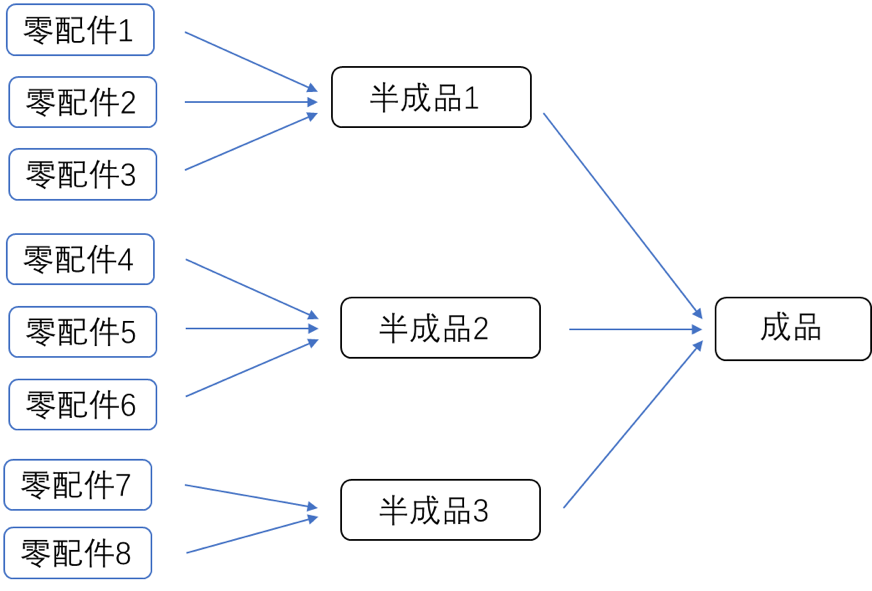
\includegraphics[width=0.5\textwidth]{微信图片_20260820103543_47_45.png}
    \caption{两道工序、八个零配件的组装结构}
    \label{fig:assembly-structure}
\end{figure}

\textbf{问题4：}  
考虑到零配件、半成品和成品的次品率通常由抽样检测估计得到，具有一定的不确定性。结合问题一的抽样方法，重新分析问题二和问题三，研究次品率估计误差对生产决策、成本、收益和产品质量的影响。








%%%%%%%%%%%%%%%%%%%%%%%%%%%%%%%%%%%%%%%%%%%%%%%%%%%%%%%%%%%%% 
\section{总体分析}

\subsection{问题一的分析———基于精确二项检验与e-progress的优化决策}

问题一要求设计一抽样检测方案用于判断是否接收供应商提供的零配件。供应商声称次品率不超过标称值$p=10\%$，企业承担检测成本。
因此，方案需同时满足两个目标：判定可靠且检测次数尽可能少。
由于每次抽检结果只有合格与次品两种状态，单个零件的检测结果可抽象为0-1随机变量，因此$n$次独立抽检中出现的次品数服从二项分布。
据此，本文首先建立起二项分布模型，通过判断当前样本$(n,k)$在次品率为10\%假设下的概率，判断结果是否反常。对于至少$k$个次品的概率低于5\%的情况，说明次品多的异常，选择拒收；
对至多$k$个次品的概率低于10\%，说明次品少的异常，选择接收；否则说明证据不足，继续抽样。

假如直接使用二项分布做多次重复判断，每次重新计算会导致出现偶然显著的情况。同时，不能很好地完成题目对检测次数尽可能少的要求。为此，本文引入e-progress方法，建立起证据分数分别记录支持拒收与接收的证据强度。
每抽检一次后更新证据分数，当拒收证据分数满足题目要求时拒收，接受证据份数满足题目要求上接收，否则继续抽检下一样品。
最终选择出合适的方案。





\subsection{问题二的分析}

问题二要求在生产过程中选择合适的检测与处理方案，使企业利益最大化。
企业的生产过程具有循环性，若成品未检测而直接进入市场，可能因为不合格而被用户退回；若不合格成品选择拆解，拆出的零配件还可以重新进入检测与装配环节。
因此，企业最终交付一件合格成品所需的成本，不仅包括第一次生产所需的费用，还包含退换货、拆解与重复生产产生的后续成本。
而且由于次品丢弃、调换、检测的成本不一，六种情况最终的最优方案并不相同。

首先，本文选择将企业最终成功交付一件合格成品作为一个完整决策周期。由于成品可能被检测出不合格，也可能在售出后被用户退回，企业还需进行报废、拆解或重新生产，因此不能只比较一次生产的成本，而应计算整个周期内的期望总成本。
接着，将零配件 1 和零配件 2 是否检测、成品是否检测以及不合格成品是否拆解分别设为决策变量。对每一种决策方案，先分析零配件进入装配环节的概率，再计算成品合格或不合格的概率，并将检测、装配、销售、调换和拆解等费用纳入成本计算。
同时，保留已有的检测信息，确保已检测的零件不再复检，未检测的零件重新判断，借助Bellman完成从当前状态到最终交付成品所需的期望成本。
在此基础上，对所有可能的拆解或检测组合进行比较，并以期望成本最小、期望利润最大为最优方案。

\subsection{问题三的分析}

问题三在问题二的基础上把决策模型推广到多道工序和多个零配件的装配系统中。
但问题三的生产结构较复杂，且最终决策由当前生产状态与后期决策相关。据此在问题二的基础上建立BOM结构对问题二进行推广，以全枚举结果选择
最优策略。



\subsection{问题四的分析}

问题四在前两问的基础上需要在次品率未知的情况下求解。考虑到抽样误差的影响，需要将统计不确定性纳入生产决策考虑。
因此，本文首先用置信区间量化不确定性，
由于次品率被低估会直接放大坏件进入装配、拆解与售后环节的风险，企业真正需要防范的是次品率偏高的情形，而非偏低，故在给定风险水平下采用单侧置信上界，
由于序贯抽样在证据充足时即停止抽检，
因此本文沿用问题一的e-progress方法得到对应的置信上界。
然而仅有单个参数的上界不足以保证整个生产系统的安全，因此通过 Bonferroni校正构造系统置信集合，最后将该置信上界代入问题二与问题三的模型中，在置信集合上对候选策略进行最坏情形重优化确定决策。
最后建立稳健决策检验模型判断当前信息是否支持稳定决策。




%%%%%%%%%%%%%%%%%%%%%%%%%%%%%%%%%%%%%%%%%%%%%%%%%%%%%%%%%%%%% 
\section{模型假设}

为简化问题，本文做出以下假设：

\begin{itemize}[itemindent=2em]
\item 假设1
\item 假设2
\item 假设3
\end{itemize}

%%%%%%%%%%%%%%%%%%%%%%%%%%%%%%%%%%%%%%%%%%%%%%%%%%%%%%%%%%%%% 

\section{符号说明}









\begin{longtable}{>{\centering\arraybackslash}p{0.14\textwidth}>{\centering\arraybackslash}p{0.68\textwidth}>{\centering\arraybackslash}p{0.08\textwidth}}

\toprule[1.5pt]
符号 & 含义 & 单位 \\
\midrule[1pt]
\endfirsthead
\multicolumn{3}{c}{\tablename~\thetable{}（续表）} \\
\midrule[1pt]
符号 & 含义 & 单位 \\
\midrule[1pt]
\endhead
\bottomrule[1.5pt]
\endfoot
\bottomrule[1.5pt]
\endlastfoot
$p$ & 实际次品率 & 概率 \\
$p_0$ & 标称次品率，本文取$0.1$ & 概率 \\
$n$ & 抽样总数 & 个 \\
$k$、$K$ & 样本中的次品数；$K=\sum_{i=1}^{n}X_i$ & 个 \\
$X_i$ & 第$i$个样品的质量结果，$X_i=1$表示次品，$X_i=0$表示合格 & --- \\
$P_{\mathrm{u}}$ & 在标称次品率下出现至少$k$个次品的概率，用于拒收判断 & 概率 \\
$P_{\mathrm{d}}$ & 在标称次品率下出现至多$k$个次品的概率，用于接收判断 & 概率 \\
$E^+$、$E^-$ & 分别支持“次品率高于”和“低于”标称值的证据分数 & --- \\
$H_0$、$H_1$ & 关于供应商次品率声明的原假设与备择假设 & --- \\
$S$ & 成品销售价格 & 元 \\
$C$ & 最终成功交付一件合格成品的期望总成本 & 元 \\
$\pi$ & 期望利润，$\pi=S-C$ & 元 \\
$p_1,p_2,p_3$ & 两种零配件及装配过程的次品率 & 概率 \\
$x_i$ & 零配件$i$是否检测的决策变量，$i=1,\dots,8$ & --- \\
$y$ & 是否检测成品的决策变量 & --- \\
$z$ & 是否拆解不合格成品的决策变量 & --- \\
$r_i$ & 拆解后回收零配件$i$是否再检测的决策变量 & --- \\
$b_i$、$c_3$ & 零配件$i$的检测成本及成品检测成本 & 元 \\
$L$、$d$ & 调换损失及拆解成本 & 元 \\
$V_s$ & 处于状态$s$时，直至成功交付所需的期望成本 & 元 \\
$g(s,a)$ & 状态$s$采取动作$a$产生的即时成本 & 元 \\
$P(s'\mid s,a)$ & 状态$s$采取动作$a$后转移至状态$s'$的概率 & 概率 \\
$C_i$ & 零配件$i$按当前策略生产一个合格件所需的期望成本，$i=1,\dots,8$ & 元 \\
$H_j$ & 第$j$个半成品，$j=1,2,3$ & --- \\
$F$ & 最终成品 & --- \\
$y_j$ & 半成品$j$是否检测的决策变量，$j=1,2,3$ & --- \\
$z_j$ & 半成品$j$不合格时是否拆解（拆解回收零配件）的决策变量 & --- \\
$y_F$ & 最终成品是否检测的决策变量 & --- \\
$z_F$ & 不合格成品是否拆解的决策变量 & --- \\
$\mathcal{D}$ & 节点的状态描述，$\mathcal{D}=(C,q,\ell,K,D,b)$ & --- \\
$\ell$ & 节点或零配件是否已被确认合格（已知合格指示） & --- \\
$\mathcal{I}_j$ & 节点$j$输入部件的下标集合 & --- \\
$p_j$、$p_F$ & 半成品$j$、成品的工序次品率 & 概率 \\
$a_j$、$a_F$ & 半成品$j$、成品的装配费 & 元 \\
$b_j$、$b_F$ & 半成品$j$、成品的单次检测费 & 元 \\
$d_j$、$d_F$ & 半成品$j$、成品的拆解费 & 元 \\
$g_j$ & 半成品$j$一次装配的成功概率 & 概率 \\
$B_j$ & 半成品$j$一次装配的即时成本 & 元 \\
$K_j$、$K_F$ & 半成品$j$、成品报废后重新生产至合格的期望成本 & 元 \\
$D_j$、$D_F$ & 半成品$j$、成品拆解后的恢复期望成本 & 元 \\
$r_{u\mid j}$ & 半成品$j$失败时其输入$u$为次品的后验概率 & 概率 \\
$R_u$ & 未知回收输入$u$的认证成本 & 元 \\
$T_j$ & 半成品$j$工序自身失败的循环修复成本 & 元 \\
$W_F$ & 成品失败后的期望处理成本 & 元 \\
$q$ & 部件或产品进入下一工序时的合格概率 & 概率 \\
$i,j$ & 零配件、半成品的编号索引 & --- \\
\label{tab:符号说明}
\end{longtable}












%%%%%%%%%%%%%%%%%%%%%%%%%%%%%%%%%%%%%%%%%%%%%%%%%%%%%%%%%%%%% 
\section{模型的建立和求解}
\subsection{问题一的模型建立与求解}
问题一要求设计一种抽样检测方案，在满足抽样次数尽可能少且判定准确的情况下作出最优决策。因此简单的二项检验不能满足题目要求。基于此本文建立了以下两层递进的模型。
\subsubsection{问题一的模型建立}
\begin{enumerate}
    \item \textbf{精确二项检验模型的建立}

    \hspace{2em}对于零件，当我们怀疑次品率超过10\%时，建立起假设检验。

    \hspace{2em}首先设原假设$H_0$：次品率$p \leq 0.1$即供应商的说法成立;备择假设$H_1$：次品率$p > 0.1$即供应商的说法不成立。

    \hspace{2em}每抽检一个零件，结果$X_i$服从0-1分布，$X_i=1$表示次品，$X_i=0$表示合格。抽检$n$个零件后，次品总数$K=\sum_{i=1}^{n}X_i$服从二项分布$B(n,p)$。

    \hspace{2em}在供应商声称$p_0=0.1$的假设下，$K \sim B(n,0.1)$，即：
    \begin{equation}
        P(K=k) = \binom{n}{k} (0.1)^k (0.9)^{n-k}
    \end{equation}

    \hspace{2em}接着进行拒收判断与接收判断。

    \hspace{2em}\textbf{拒收判断：}计算当前样本$(n,k)$在$p=0.1$假设下出现至少$k$个次品的概率：
    \begin{equation}
        P_{\text{u}} = P(K \geq k \mid p=0.1) = \sum_{i=k}^{n} \binom{n}{i} (0.1)^i (0.9)^{n-i}
    \end{equation}
    \hspace{2em}若$P_{\text{up}} < 5\%$，说明在次品率$=10\%$的假设下，当前结果过于反常，拒绝$H_0$，判定为拒收。

    \hspace{2em}\textbf{接收判断：}当认为次品率可能低于10\%时，建立反向假设：
    原假设$H_0'$：次品率$p \geq 0.1$；备择假设$H_1'$：次品率$p < 0.1$。

    \hspace{2em}计算至多$k$个次品的概率：
    \begin{equation}
        P_{\text{d}} = P(K \leq k \mid p=0.1) = \sum_{i=0}^{k} \binom{n}{i} (0.1)^i (0.9)^{n-i}
    \end{equation}
     \hspace{2em}若$P_{\text{d}} < 10\%$，说明在"次品率$=10\%$"的假设下，合格品多得异常，拒绝$H_0'$，判定为接收。

     \hspace{2em}对于任意$(n,k)$，存在三种可能：
    \begin{itemize}[leftmargin=4em]
        \item $P_{\text{u}} < 5\%$：拒收
        \item $P_{\text{d}} < 10\%$：接收
        \item 两者均不满足：证据不足，继续抽样
    \end{itemize}

     \hspace{2em}但是，精确二项检验只通过重复查看判断次品的可信度，一方面，重复查看会增加偶然显著性，导致错误率累计，结果出现较大偏差；另一方面，
     这种方法不能满足题目中观测次数尽可能少的需求。
     因此需要引入序贯决策方法。

    \item \textbf{e-process模型的建立}
    
    \hspace{2em}为了解决重复查看带来的误差累积问题，本文引入e-process序贯决策方法。

    \hspace{2em}首先建立两个累计证据分数：
    \begin{itemize}[leftmargin=4em]
        \item $E^+$：支持次品率$>10\%$的证据强度，初始值为1。
        \item $E^-$：支持次品率$<10\%$的证据强度，初始值为1。
    \end{itemize}

    \hspace{2em}每抽检一个零件，根据结果更新分数。
而更新因子的确定基于以下考虑：

\hspace{2em}（1）当抽到次品时，该结果对"次品率$>10\%$"提供强证据，因此$E^+$乘以一个大于1的因子、$E^-$乘以一个小于1的因子。取因子10和0.1，即观察到一次次品，相当于将支持"次品率$>10\%$"的证据强度提升为原来的10倍，同时将支持"次品率$<10\%$"的证据强度压缩为原来的0.1倍。

\hspace{2em}（2）当抽到合格品时，该结果对"次品率$<10\%$"提供弱证据，因此$E^-$乘以一个大于1的因子、$E^+$乘以一个小于1的因子。取因子$10/9$和$0.9$，即观察到一次合格品，相当于将支持"次品率$<10\%$"的证据强度提升为原来的$10/9$倍，同时将支持"次品率$>10\%$"的证据强度压缩为原来的$0.9$倍。

\hspace{2em}因子取值的核心依据是Ville不等式：若原假设成立（即次品率$p \leq 0.1$），则$E^+$超过任意正数$c$的概率不超过$1/c$。因此，设定门槛$c=20$，可得$P(E^+ \geq 20) \leq 1/20 = 5\%$，即误拒风险不超过$5\%$，对应$95\%$的置信度。同理，$P(E^- \geq 10) \leq 1/10 = 10\%$，即误收风险不超过$10\%$，对应$90\%$的置信度。

\hspace{2em}据此得到更新规则与停止规则。

    \hspace{2em}
\textbf{更新规则：}

 \hspace{2em}当抽到次品时：
    \begin{equation}
        E^+ \leftarrow E^+ \times 10, \quad E^- \leftarrow E^- \times 0.1
    \end{equation}

    \hspace{2em}当抽到合格品时：
    \begin{equation}
        E^- \leftarrow E^- \times \frac{10}{9}, \quad E^+ \leftarrow E^+ \times 0.9
    \end{equation}

    \hspace{2em}\textbf{停止规则：}

    \begin{itemize}[leftmargin=4em]
        \item 若$E^+ \geq 20$，则拒收
        \item 若$E^- \geq 10$，则接收
        \item 否则，继续抽取下一个零件。
    \end{itemize}

\end{enumerate}


通过e-progress的辅助，可以求得第一问的企业最佳抽样检测方案。











\subsubsection{问题一的求解结果}

根据所建立的 e-process 模型，得到序贯抽样边界如表~\ref{tab:sequential-boundaries}所示，表中给出了不同抽样量$n$下判定接收或拒收的临界次品数$k$。

\begin{table}[H]
\centering
\caption{序贯抽样边界（部分）}
\label{tab:sequential-boundaries}
\begin{tabularx}{\textwidth}{CCCC}
\toprule[1.5pt]
$n$ & 接收边界$k$ & 拒收边界$k$ \\
\midrule[1pt]
$2$ & --- & $2$ \\
$34$ & $0$ & $10$ \\
$40$ & $0$ & $11$ \\
$50$ & $0$ & $13$ \\
$80$ & $2$ & $18$ \\
$100$ & $3$ & $21$ \\
$160$ & $7$ & $30$ \\
$200$ & $10$ & $36$ \\
$500$ & $33$ & $75$ \\
\bottomrule[1.5pt]
\end{tabularx}
\end{table}

从表中可以看出，序贯抽样边界随着$n$的增大而逐渐放宽，最早在$n=2$时即可达到拒收边界，最早在$n=34$时达到接收边界。

\begin{figure}[H]
\centering
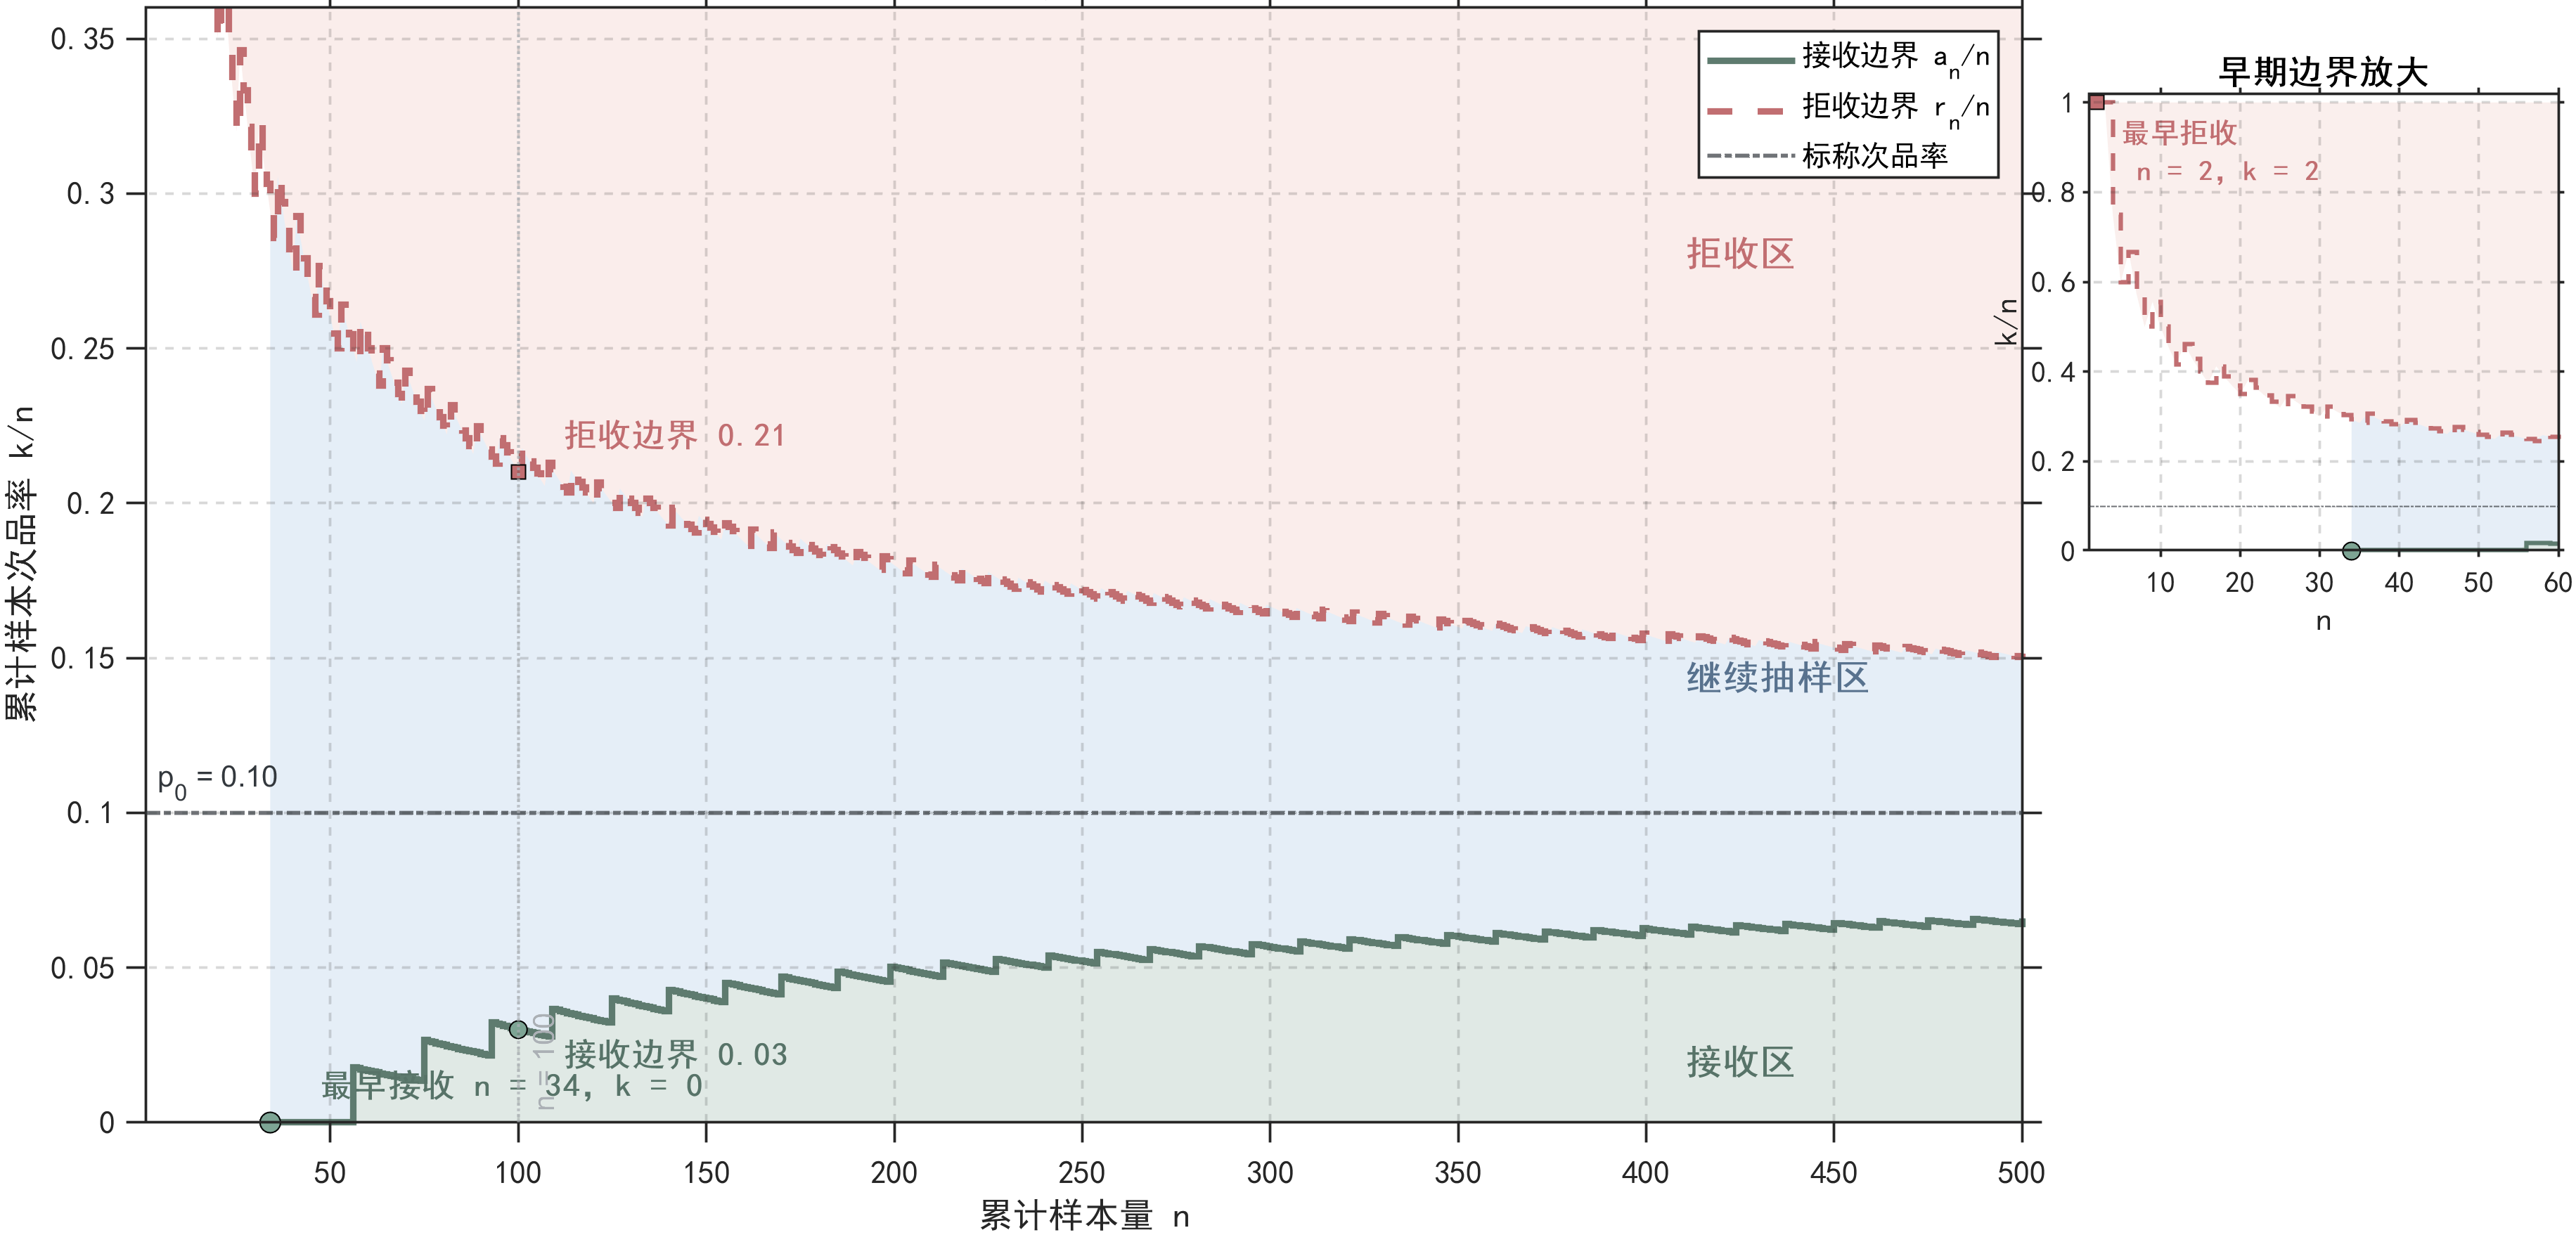
\includegraphics[width=0.85\textwidth]{figures/fig3_decision_regions.png}
\caption{序贯停止边界与三决策区域}
\label{fig:decision-regions}
\end{figure}

序贯决策域由接收、继续抽样和拒收三个区域组成。边界在小样本阶段较宽，以避免有限信息造成误判；随样本量增加，接收边界单调上移、拒收边界逐步下移，并共同逼近标称次品率$p_0=0.10$，从而提高临界区域的判别能力。最早拒收发生在$n=2$、$k=2$，最早接收发生在$n=34$、$k=0$。

此外，将序贯停止边界与固定样本精确二项检验边界进行对比，结果如图~\ref{fig:boundary-compare}所示：

\begin{figure}[H]
\centering
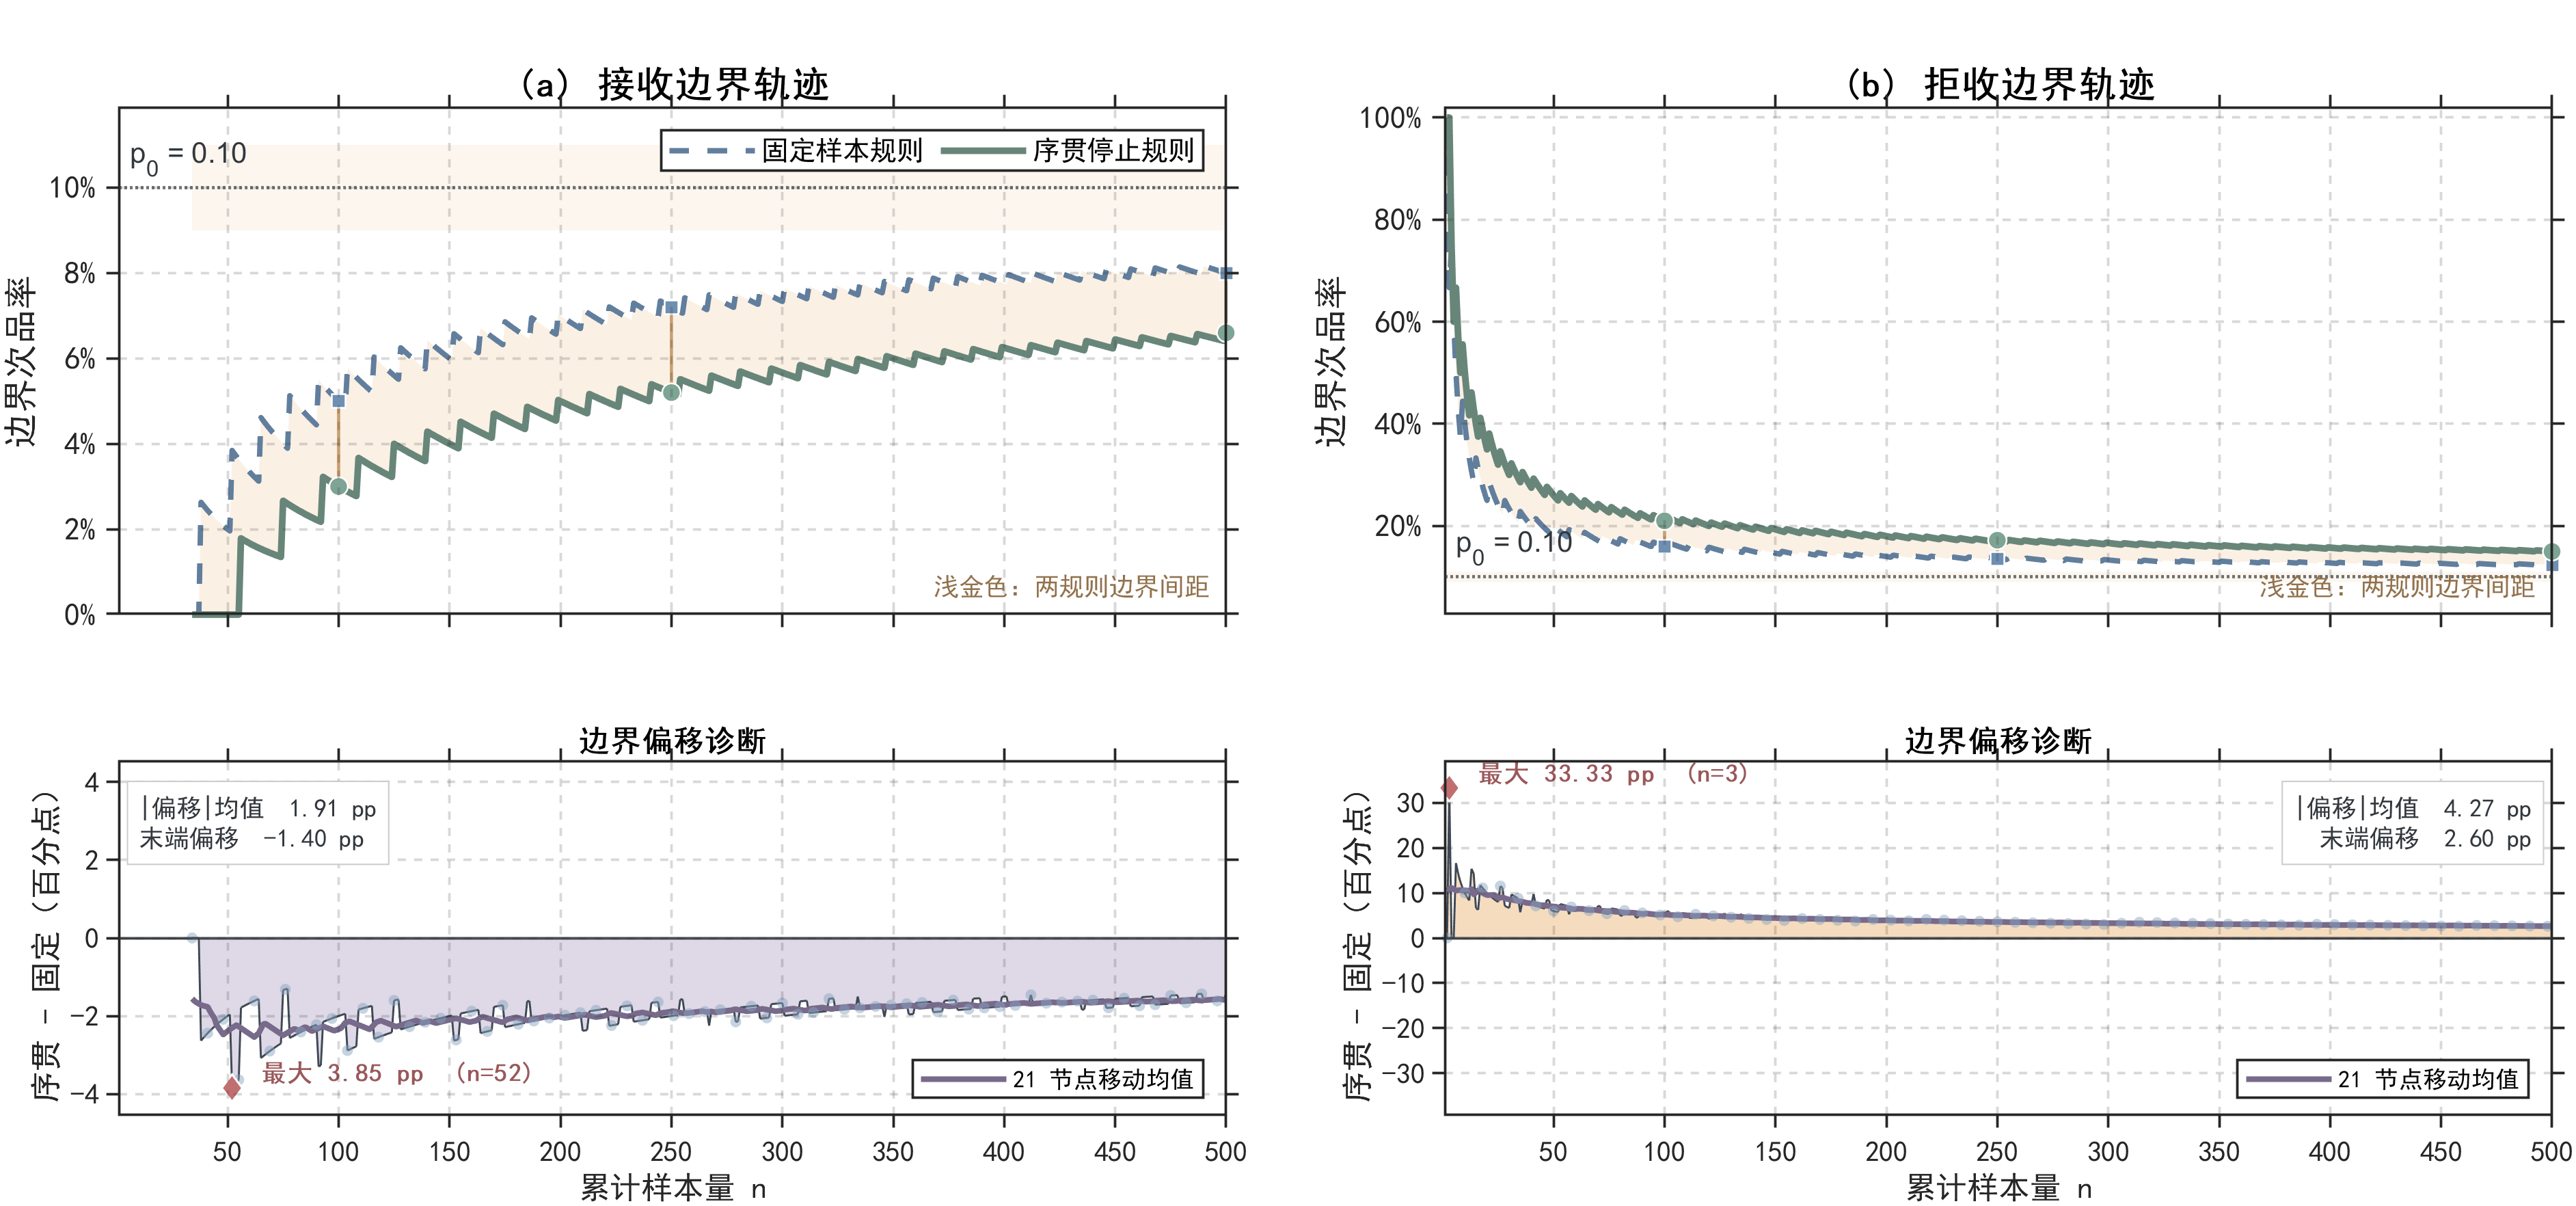
\includegraphics[width=0.85\textwidth]{figures/fig2_boundary_compare.png}
\caption{固定样本与序贯停止边界对比}
\label{fig:boundary-compare}
\end{figure}

固定样本规则与序贯规则的边界变化趋势一致，但在小样本阶段存在一定差异；随着样本量增加，两者的边界逐渐接近。





同时，采用动态概率递推方法对方案进行性能评估。递推流程如图~\ref{fig:dp-flow}所示。

\begin{figure}[H]
\centering
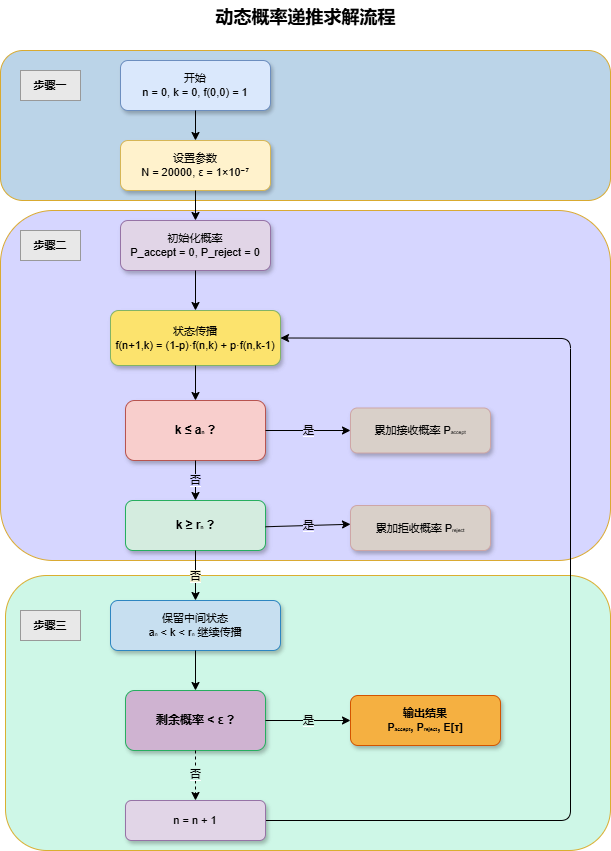
\includegraphics[width=0.8\textwidth]{动态概率递推流程图.png}
\caption{动态概率递推求解流程}
\label{fig:dp-flow}
\end{figure}

设定真实次品率$p$分别取$5\%$、$8\%$、$10\%$、$12\%$、$20\%$。
递推结果如表~\ref{tab:simulation-results}所示：

\begin{longtable}{>{\centering\arraybackslash}p{0.2\textwidth}>{\centering\arraybackslash}p{0.25\textwidth}>{\centering\arraybackslash}p{0.25\textwidth}>{\centering\arraybackslash}p{0.3\textwidth}}
\caption{不同真实次品率下的方案性能}
\label{tab:simulation-results}\\
\toprule[1.5pt]
真实次品率 $p$ & 接收概率 & 拒收概率 & 条件期望样本量 \\
\midrule[1pt]
\endfirsthead

\multicolumn{4}{c}{表~\ref{tab:simulation-results}（续）} \\
\toprule[1.5pt]
真实次品率 $p$ & 接收概率 & 拒收概率 & 条件期望样本量 \\
\midrule[1pt]
\endhead

\bottomrule[1.5pt]
\endfoot

\bottomrule[1.5pt]
\endlastfoot

$5\%$ & $99.64\%$ & $0.36\%$ & $161$ \\
$8\%$ & $98.76\%$ & $1.24\%$ & $1292$ \\
$10\%$ & $9.29\%$ & $2.99\%$ & $677$ \\
$12\%$ & $2.16\%$ & $97.84\%$ & $2846$ \\
$20\%$ & $0.05\%$ & $99.95\%$ & $103$ \\
\end{longtable}

结果分析：当$p=5\%$和$p=20\%$时，方案能以较少的样本做出正确判断；当$p=10\%$时，有$87.72\%$的路径在$20000$步内未做出判定，这说明越接近质量判定边界，越难判断，需要更多样本信息，符合统计直觉。

真实次品率对检验性能与检测成本的影响如图~\ref{fig:perf-cost}所示：

\begin{figure}[H]
\centering
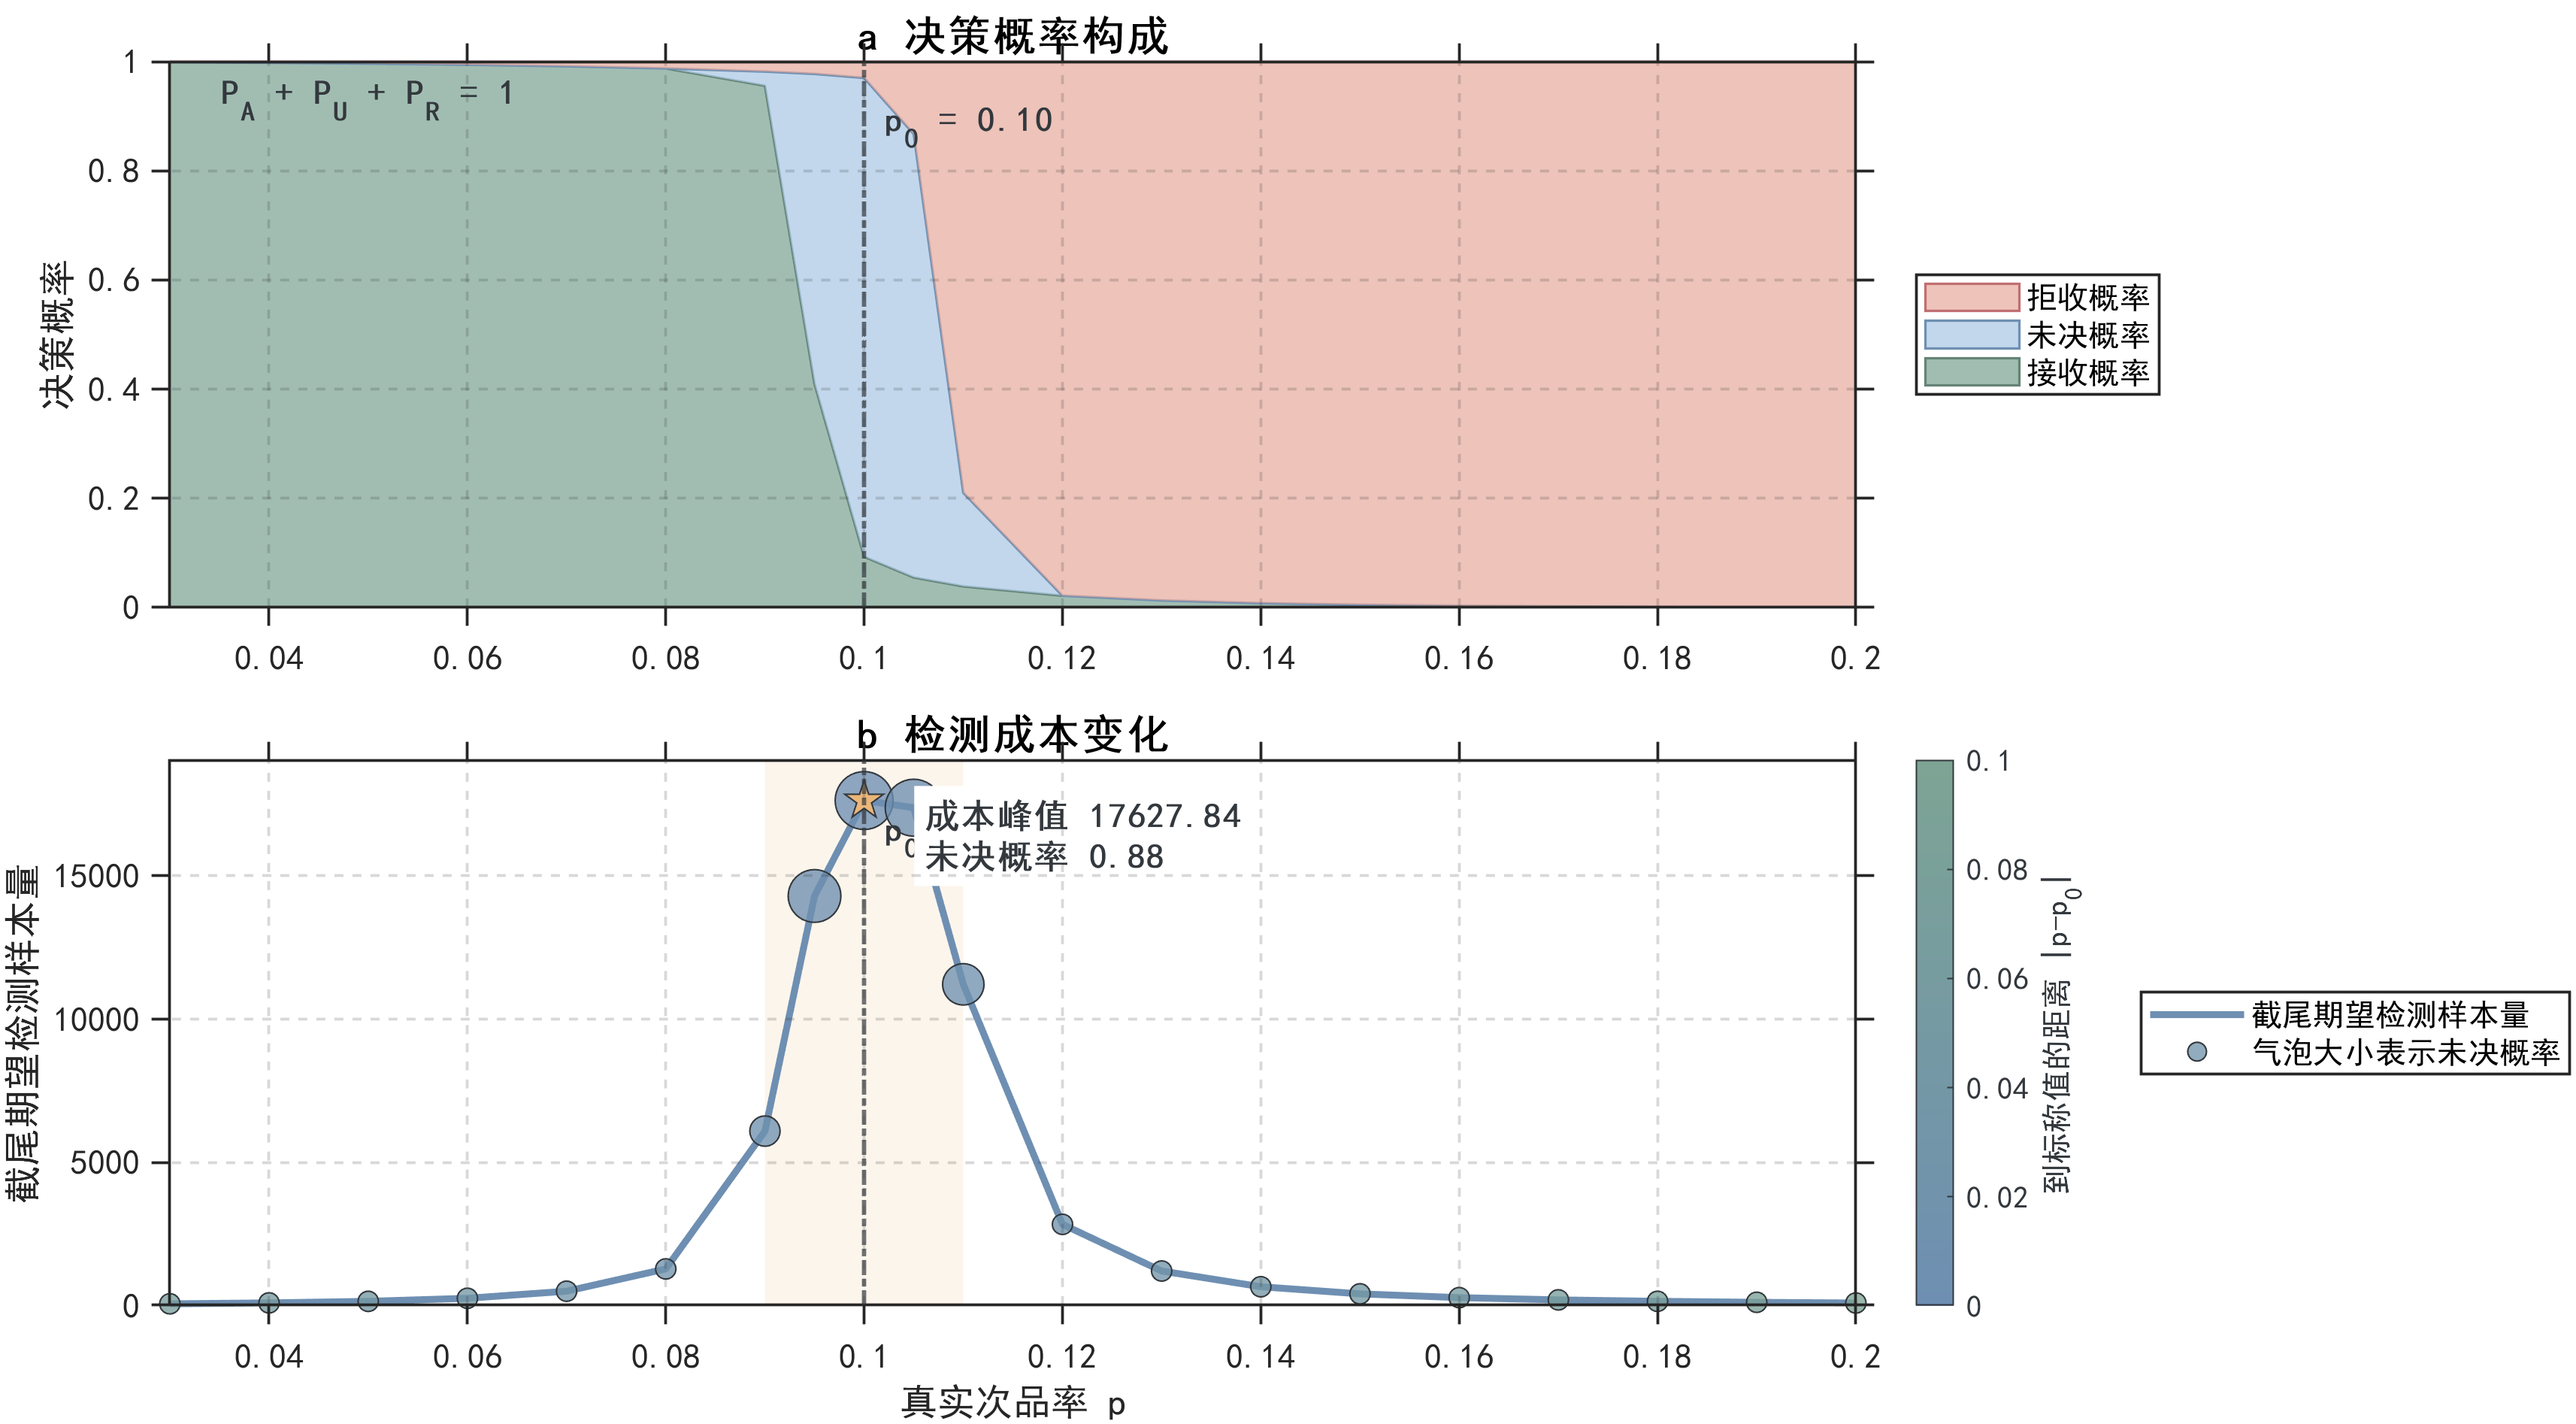
\includegraphics[width=0.85\textwidth]{figures/fig4_performance_cost.png}
\caption{真实次品率对检验性能与检测成本的影响}
\label{fig:perf-cost}
\end{figure}

检测成本关于真实次品率呈明显的阈值峰值结构。在标称值$p_0=0.10$附近，两类假设难以区分，模型需要更多观测积累证据，截尾期望检测样本量达到约$17627$；远离阈值后，判别信号增强，期望检测样本量迅速下降。这说明序贯机制能够在保持临界区域谨慎性的同时，减少易判别批次的检测次数。

\subsubsection{问题一的模型检验与灵敏度分析}

为进一步验证方案的可靠性，从以下两个维度进行检验：

\textbf{（1）错误率控制检验} 

\begin{figure}[H]
\centering
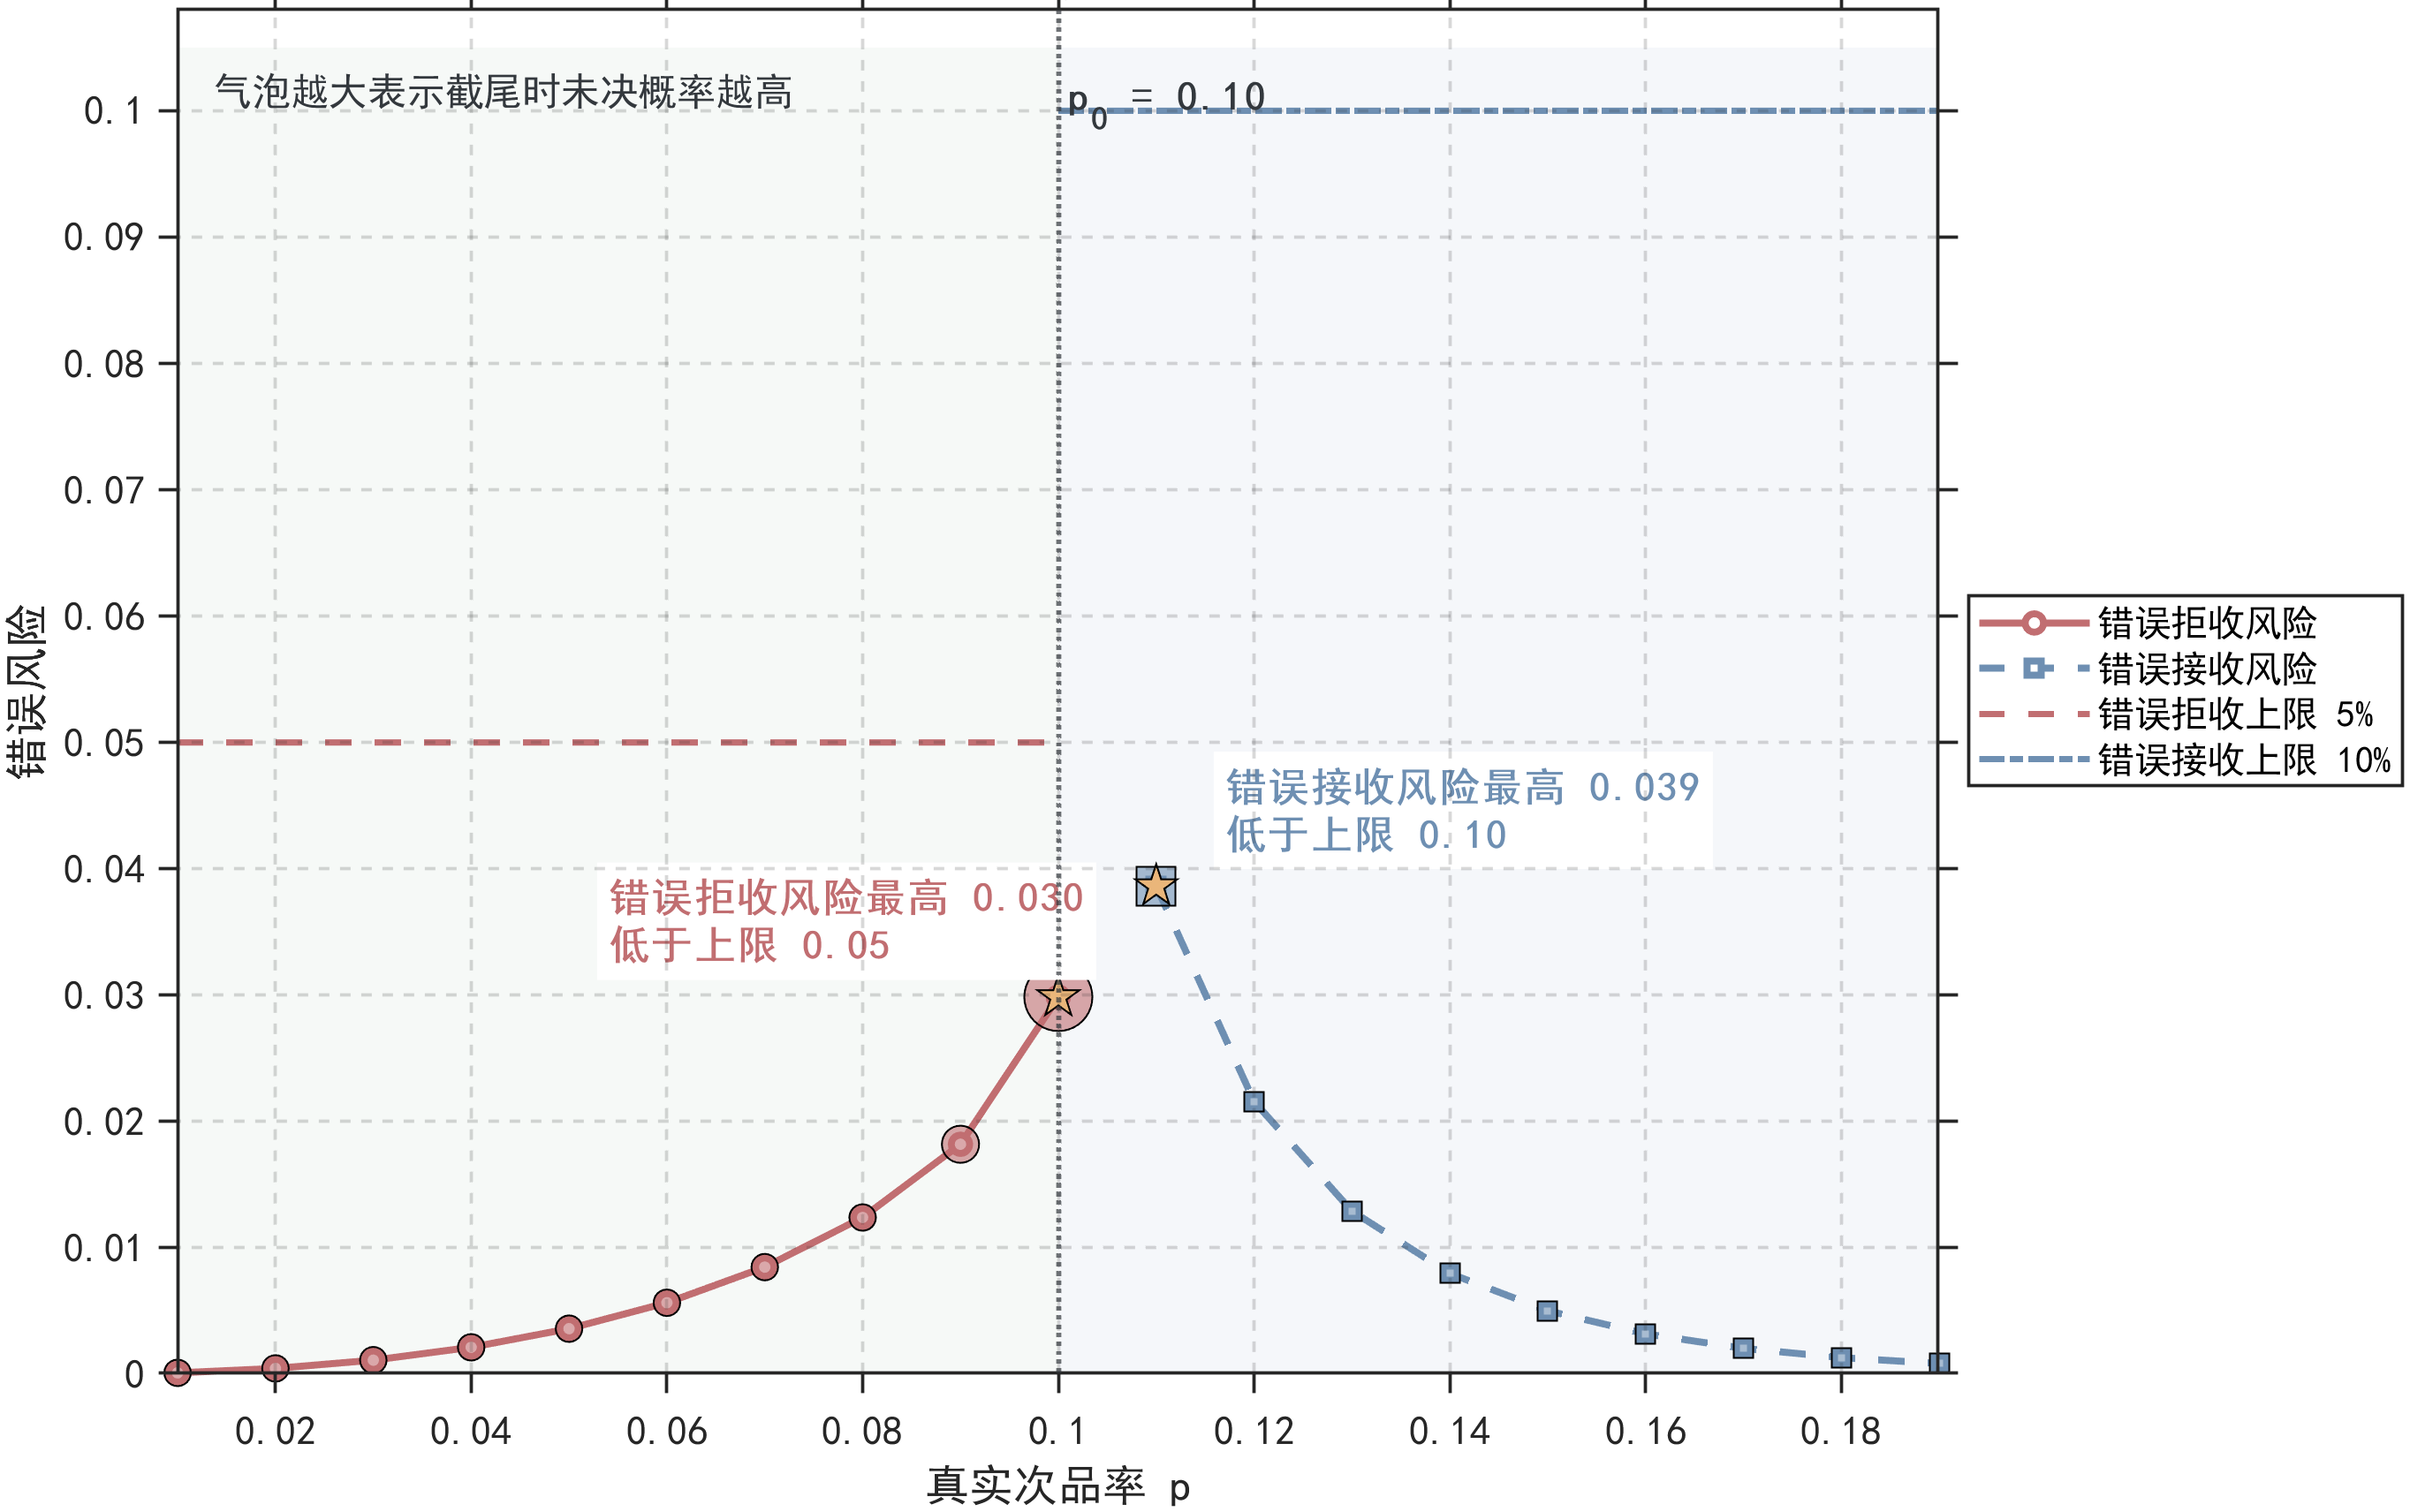
\includegraphics[width=0.85\textwidth]{figures/fig5_risk_control.png}
\caption{序贯检验错误风险控制验证}
\label{fig:risk-control}
\end{figure}
在$p\leq 10\%$的范围内，误拒风险均未超过$5\%$的理论上限，具体而言，$p=5\%$时误拒风险为$0.36\%$，$p=10\%$时误拒风险为$2.99\%$；在$p\geq 10\%$的范围内，误收风险均未超过$10\%$的理论上限，$p=12\%$时误收风险为$2.16\%$，$p=20\%$时误收风险为$0.05\%$。全部网格点均通过了理论上限检查，验证了方案对两类错误的有效控制，如图~\ref{fig:risk-control}所示：



\textbf{（2）样本效率检验}

方案呈现出明显的边界效应，$p=5\%$时条件期望样本量仅$161$，$p=20\%$时仅$103$，而$p=10\%$附近则有$87.72\%$的路径在$20000$步内无法判定，表明方案在证据充分时尽早停止、边界模糊时充分采样之间取得了合理平衡。

检验结果表明，该方案满足题目要求的检测次数尽可能少和$95\%$置信度拒收、$90\%$置信度接收的双重目标，可用于实际生产中的零配件验收环节。


\textbf{（3）灵敏度分析}

进一步分析真实次品率与置信水平对检测成本的联合影响，如图~\ref{fig:sensitivity}所示：

\begin{figure}[H]
\centering
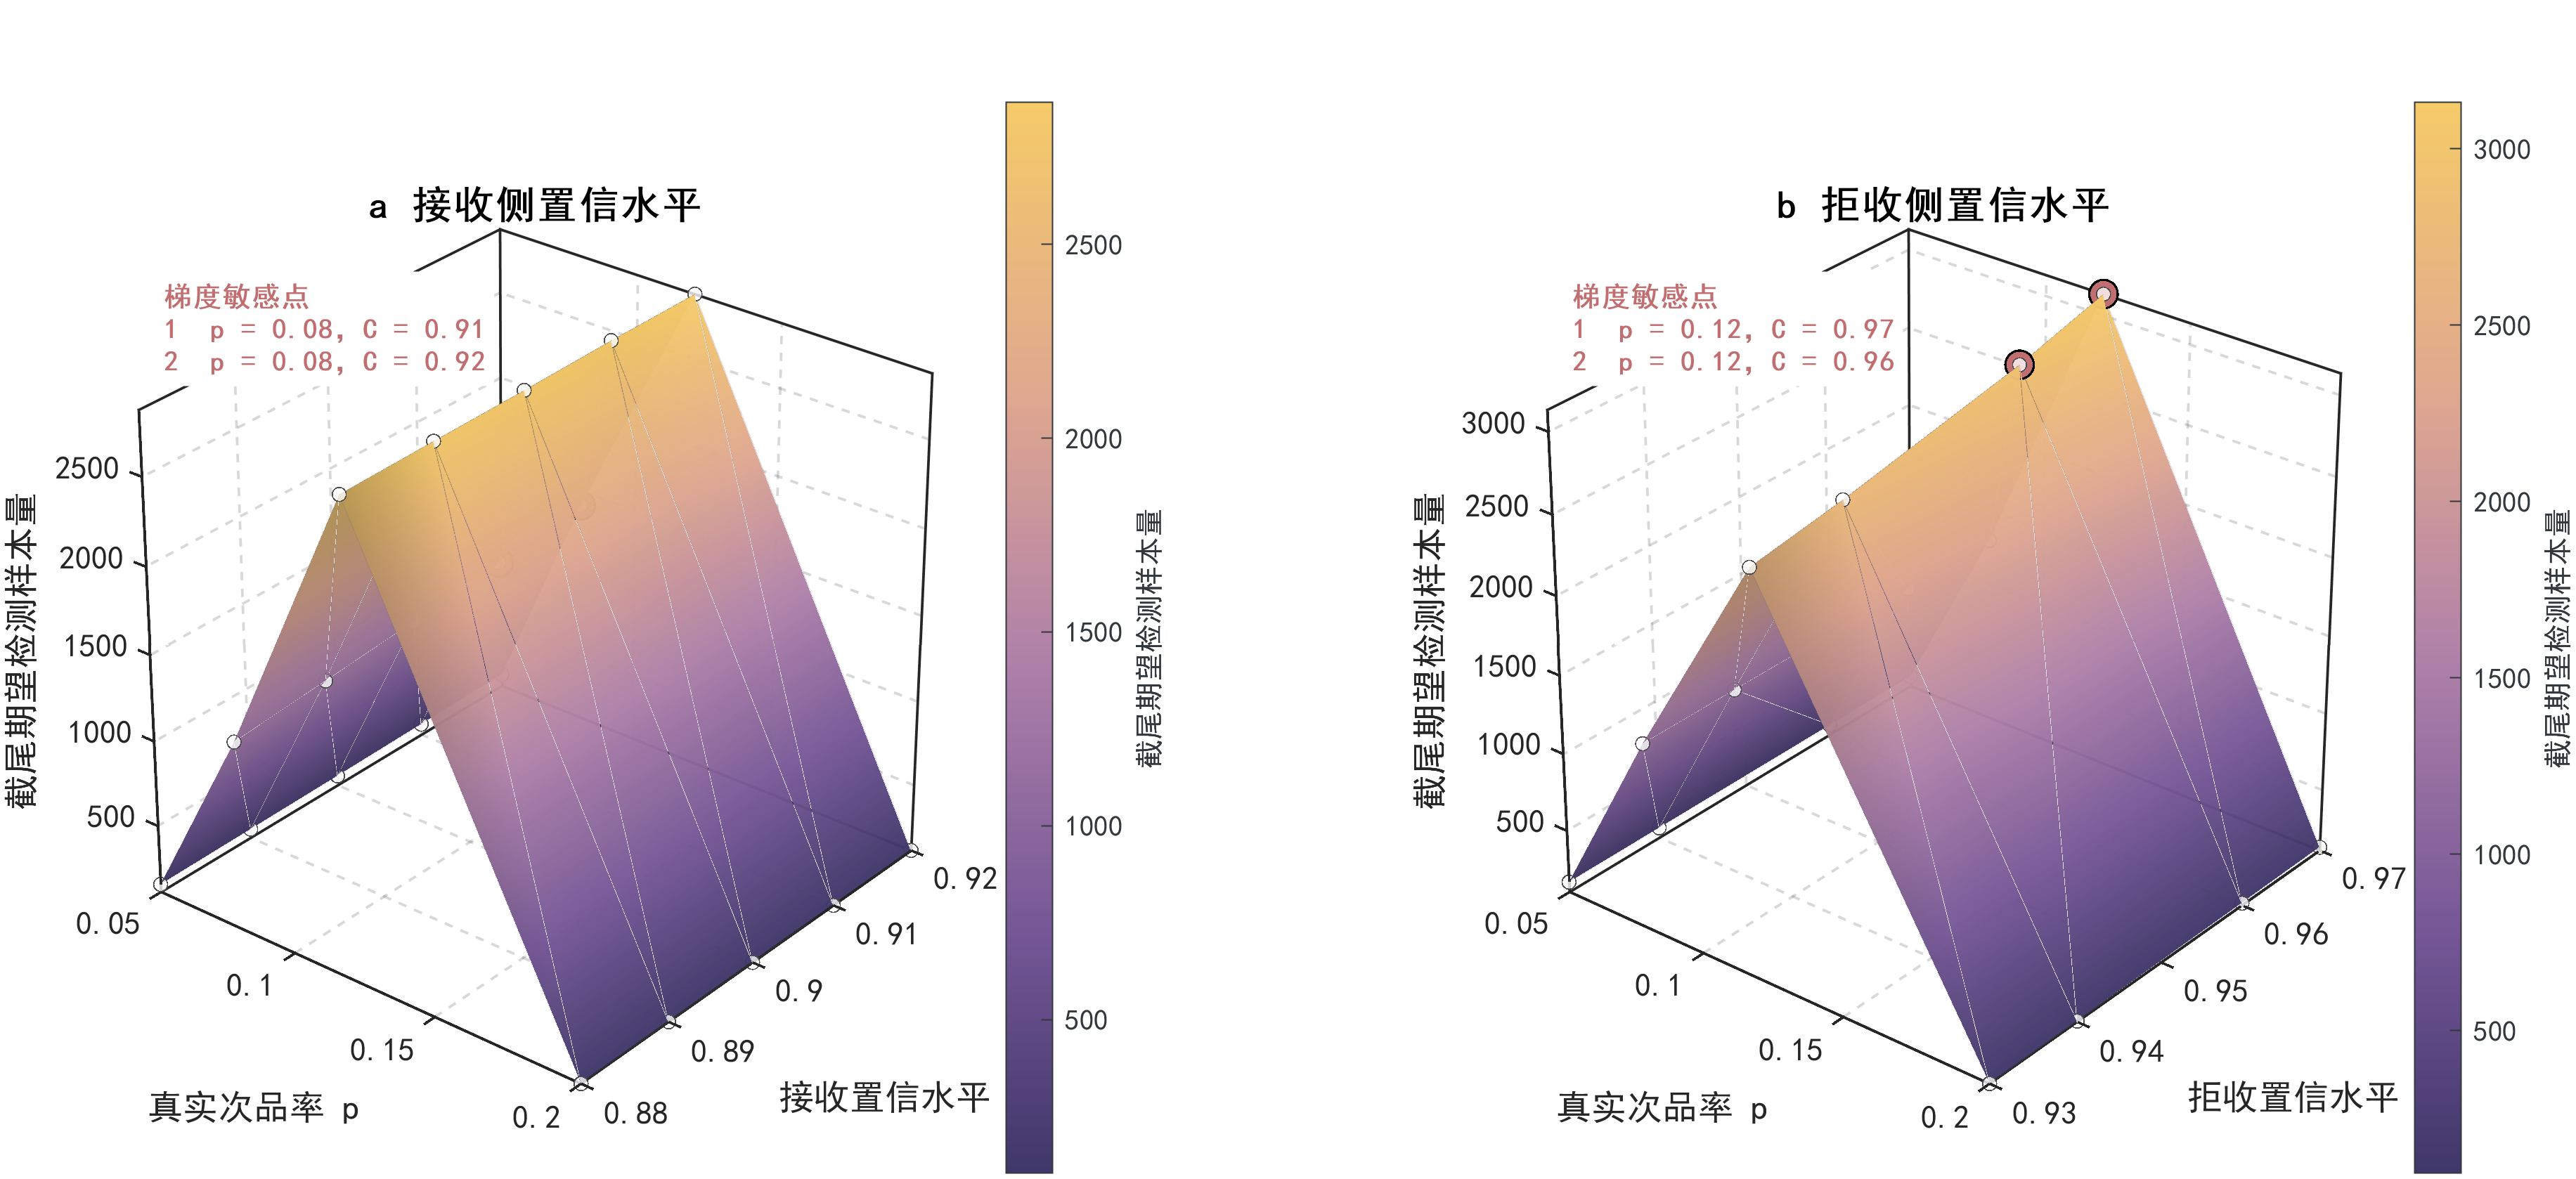
\includegraphics[width=0.85\textwidth]{figures/fig6_sensitivity.png}
\caption{真实次品率与置信水平对检测成本的联合影响}
\label{fig:sensitivity}
\end{figure}

联合敏感性分析表明，检测成本不仅受真实次品率影响，也会随两侧置信水平发生局部陡变。基于置信水平方向局部梯度识别出的敏感节点主要位于阈值邻域两侧，说明提高置信要求会在难判别区域显著增加检测成本。该结果为风险水平与抽检代价之间的参数权衡提供了依据。


\subsubsection{问题一的结论}

针对问题一，本文的结论如下：

\textbf{方案：} 采用 e-process 序贯抽样方案。初始化 $E^+=1$、$E^-=1$，逐件抽检，每抽一个零件后更新证据分数，当 $E^+\geq 20$ 时拒收，$E^-\geq 10$ 时接收，否则继续抽检。

\textbf{结果：}

（1）在 $95\%$ 信度下拒收：当 $E^+\geq 20$ 时判定拒收。例如抽检 $2$ 个均为次品即可拒收；抽检 $100$ 个时次品数达到 $21$ 个则拒收。

（2）在 $90\%$ 信度下接收：当 $E^-\geq 10$ 时判定接收。例如抽检 $34$ 个均无次品即可接收；抽检 $100$ 个时次品数不超过 $3$ 个则接收。

\textbf{方案性能：} 真实次品率 $p=5\%$ 时，接收概率 $99.64\%$，条件期望样本量 $161$；$p=20\%$ 时，拒收概率 $99.95\%$，条件期望样本量 $103$。$p=10\%$ 时误拒风险 $2.99\%$，$p=12\%$ 时误收风险 $2.16\%$，两类错误均控制在题目要求的 $5\%$ 和 $10\%$ 以内。






%%%%%%%%%%%%%%%%%%%%%%%%%%%%%%%%%%%%%%%%%%%%%%%%%%%%%%%%%%%%% 
\subsection{问题二的模型建立与求解}

问题二中需要求解在生产过程中涉及循环的零配件检测与处理方案，使得企业最终交付一件合格产品时的平均利润最大。针对这一过程，本文建立生产循环检测与拆解决策优化模型。
企业需要对零配件是否检测、对成品是否检测，以及对不合格成品是否进行拆解。
不同决策会会影响检测费用、装配费用、报废损失、调换损失和零配件的重复利用价值，并同时受到多种因素的影响。
基于此，本文建立起以下模型求解。









\subsubsection{问题二的模型建立}



\textbf{1. 检测与拆解决策模型的建立}

本问题的决策并非一次性完成，而是随着零配件检测结果、装配结果和成品处置结果逐步展开。为此，本文
构造了以下六个决策变量。

首先，在零配件进入装配环节之前，企业需要决定是否对两个零配件进行检测。令
\begin{equation}
x_i=
\begin{cases}
1, & \text{检测零配件 }i\\
0, & \text{不检测零配件 }i
\end{cases}
\qquad i=1,2
\end{equation}

检测零配件可以提前剔除不合格零配件，但会产生额外检测费用；不检测则节省检测费用，但不合格零配件可能进入装配环节，增加后续生产和售后风险。

完成装配后，企业需要决定是否对成品进行检测。令
\begin{equation}
y=
\begin{cases}
1, & \text{检测成品}\\
0, & \text{不检测成品}
\end{cases}
\end{equation}

当$y=1$时，不合格成品可以在销售前被识别，从而避免用户购买后的调换损失；当$y=0$时，不合格成品可能直接流入市场，并在售后阶段产生调换损失。

对于检测或售后过程中发现的不合格成品，企业还需要决定是直接报废，还是拆解后回收其中的零配件。令
\begin{equation}
z=
\begin{cases}
1, & \text{拆解不合格成品并尝试回收零配件}\\
0, & \text{直接报废不合格成品}
\end{cases}
\end{equation}

若选择报废，企业需要重新采购一套零配件并进入下一轮生产；若选择拆解，则保留回收零配件的质量信息，并将其送入下一轮装配流程。

拆解后的零配件并不一定需要重复检测。对于回收后质量仍未知的零配件，企业需要进一步决定是否进行再检测。令
\begin{equation}
r_i=
\begin{cases}
1, & \text{检测拆解回收后的零配件 }i\\
0, & \text{不检测拆解回收后的零配件 }i
\end{cases}
\qquad i=1,2
\end{equation}

若回收零配件已经被确认合格，则不再重复检测；若其质量未知且$r_i=1$，则对其进行检测；若$r_i=0$，则保留其未知质量状态，并直接参与后续装配。因此，$r_1$和$r_2$体现的是拆解回收环节中的信息处理策略，而不是首次生产阶段的检测决策。

综上，一个完整策略表示为
\begin{equation}
\boldsymbol{x}=(x_1,x_2,y,z,r_1,r_2)
\end{equation}
其中前四个变量决定首次生产过程中的检测与不合格品处置方式，后两个变量决定拆解回收后的零配件处理方式。各变量均为二元变量，具体表示为

\begin{equation}
x_1,x_2,y,z,r_1,r_2 \in \{0,1\}
\end{equation}





\textbf{2. 期望利润目标模型的建立}

本文选择将企业成功交付一件合格成品作为完整决策周期。但由于成品可能在检测环节判断为不合格，也可能因为售后问题被退回，因此不能仅比较单次生产，必须将整个决策周期内的期望总成本作为评价标准。

故设市场售价为$S$，企业最终成功交付一件合格成品所需的期望总成本为$C$，则期望利润为：
\begin{equation}
\max_{\boldsymbol{x}\in\{0,1\}^6} \pi(\boldsymbol{x}) = S - C(\boldsymbol{x})
\end{equation}
其中$\boldsymbol{x}=(x_1,x_2,y,z,r_1,r_2)$为策略向量，$C(\boldsymbol{x})$为该策略下的期望总成本，包括零配件购买成本、检测成本、装配成本、成品检测成本、调换损失、拆解成本和报废成本。对于每种策略，选取$\pi$最大的作为最佳策略。

对于每一个有效策略，模型按照以下阶段依次计算其期望总成本，如图~\ref{fig:cost-flow}所示：
\begin{figure}[H]
    \centering
    \definecolor{flowblue}{RGB}{218,232,252}
    \begin{tikzpicture}[
        font=\footnotesize,
        box/.style={rectangle, draw=black, thick, text centered, align=center, inner sep=4pt,
                    minimum width=2.5cm, minimum height=1.1cm, fill=flowblue},
        node distance=1.2cm]
        \node[box] (s1) {零配件采购与检测\\$x_1,\ x_2$};
        \node[box, right=of s1] (s2) {装配};
        \node[box, right=of s2] (s3) {成品检测或销售\\$y$};
        \node[box, right=of s3] (s4) {报废或拆解\\$z$};
        \node[box, right=of s4] (s5) {回收零配件再利用\\$r_1,\ r_2$};
        \draw[arrow] (s1) -- (s2);
        \draw[arrow] (s2) -- (s3);
        \draw[arrow] (s3) -- (s4);
        \draw[arrow] (s4) -- (s5);
    \end{tikzpicture}
    \caption{生产周期中各阶段的成本计算流程}
    \label{fig:cost-flow}
\end{figure}

理论上，六个二元变量构成$2^6=64$个原始策略。需要注意的是，当$z=0$时，不合格成品直接报废，不会进入拆解回收环节，此时$r_1$和$r_2$不会被实际触发，属于冗余变量。因此，模型首先对$64$个原始策略进行统一编码，并将$z=0$时的回收决策规范化为
\begin{equation}
r_1=r_2=0
\end{equation}

最终得到$40$个具有实际区别的有效策略。

\textbf{3. 成品质量概率模型的建立}

题目给出的成品次品率$p_3$是指两个零配件均合格时，装配过程本身产生次品的概率。因此成品合格率需根据零配件检测情况分别计算：
\begin{equation}
P_{\text{合格}} =
\begin{cases}
(1-p_1)(1-p_2)(1-p_3), & \text{两个零配件均未检测} \\
(1-p_2)(1-p_3), & \text{零配件1已检测合格} \\
1-p_3, & \text{两个零配件均已检测合格}
\end{cases}
\end{equation}

\textbf{4. 生产循环状态Bellman转移模型的建立}

由于生产具有循环性，后期决策是当前状态与后续期望成本综合决定，据此
将整个生产过程建模为马尔可夫链，每个状态表示企业当前拥有的零件质量信息。主要状态包括：两个零件质量均未知、部分零件已知合格、全部零件已知合格、已完成装配等待成品检测或销售、最终成功交付。企业每采取一个动作，系统以一定概率进入下一状态，同时产生相应成本。

对于每个状态，定义$V_s$为从该状态到最终成功交付的期望总成本，建立Bellman方程：
\begin{equation}
V_s=g(s,a)+\sum_{s'}P(s'|s,a)V_{s'}
\end{equation}
其中，$g(s,a)$表示系统处于当前状态$s$并采取动作$a$时产生的即时成本；$s'$表示一次决策后可能到达的下一状态，
$P(s'|s,a)$表示在当前状态$s$下采取动作$a$后转移至下一状态$s'$的概率；$V_{s'}$表示从下一状态$s'$继续运行直至最终成功交付所需的期望成本。

对所有暂态建立上述方程，可以得到关于各状态价值函数的线性方程组，求解即可得到该策略下从初始状态出发的期望总成本$C$。


\textbf{5. 多方案期望利润优化模型的建立}

由于决策变量均为$0$-$1$变量，六位策略空间共$64$种候选方案。采用全枚举方法逐一求解每种策略的期望成本，选取期望利润最高的方案作为最优策略。该方法保证找到的一定是当前策略空间内的全局最优解。















\subsubsection{问题二的求解结果}



对每一情形枚举全部候选策略并比较期望利润，得到的最优策略及结果如表~\ref{tab:q2-optimal}所示。

\small
\begin{longtable}{@{}>{\centering\arraybackslash}p{0.05\textwidth} >{\centering\arraybackslash}p{0.08\textwidth} >{\centering\arraybackslash}p{0.09\textwidth} >{\raggedright\arraybackslash}p{0.24\textwidth} >{\centering\arraybackslash}p{0.09\textwidth} >{\centering\arraybackslash}p{0.09\textwidth} >{\centering\arraybackslash}p{0.08\textwidth} >{\centering\arraybackslash}p{0.05\textwidth}@{}}
\caption{六种情形的最优决策结果}
\label{tab:q2-optimal}\\
\toprule[1.5pt]
情形 & 四位策略 & 六位策略 & 决策内容 & 期望成本 & 期望利润 & 次优策略 & 利润差 \\
\midrule[1pt]
\endfirsthead
\multicolumn{8}{c}{\tablename~\thetable{}（续表）} \\
\midrule[1pt]
情形 & 四位策略 & 六位策略 & 决策内容 & 期望成本 & 期望利润 & 次优策略 & 利润差 \\
\midrule[1pt]
\endhead
\bottomrule[1.5pt]
\endfoot
\bottomrule[1.5pt]
\endlastfoot
1 & 1001 & 100101 & 1检、2不检、成品不检、拆解 & 37.16 & \textbf{18.84} & 0001 & 0.31 \\
2 & 1101 & 110100 & 1、2均检、成品不检、拆解 & 44.00 & \textbf{12.00} & 1001 & 1.48 \\
3 & 1011 & 101101 & 1检、2不检、成品检、拆解 & 39.53 & \textbf{16.47} & 0011 & 0.05 \\
4 & 1111 & 111100 & 1、2均检、成品检、拆解 & 41.25 & \textbf{14.75} & 0111 & 1.96 \\
5 & 0101 & 010110 & 1不检、2检、成品不检、拆解 & 41.04 & \textbf{14.96} & 0111 & 0.31 \\
6 & 0000 & 000000 & 1、2、成品均不检、报废 & 34.32 & \textbf{21.68} & 1000 & 0.35 \\
\end{longtable}
\normalsize

对六种情形进行分析，得到图~\ref{fig:q2-fig2}。
\begin{figure}[H]
    \centering
    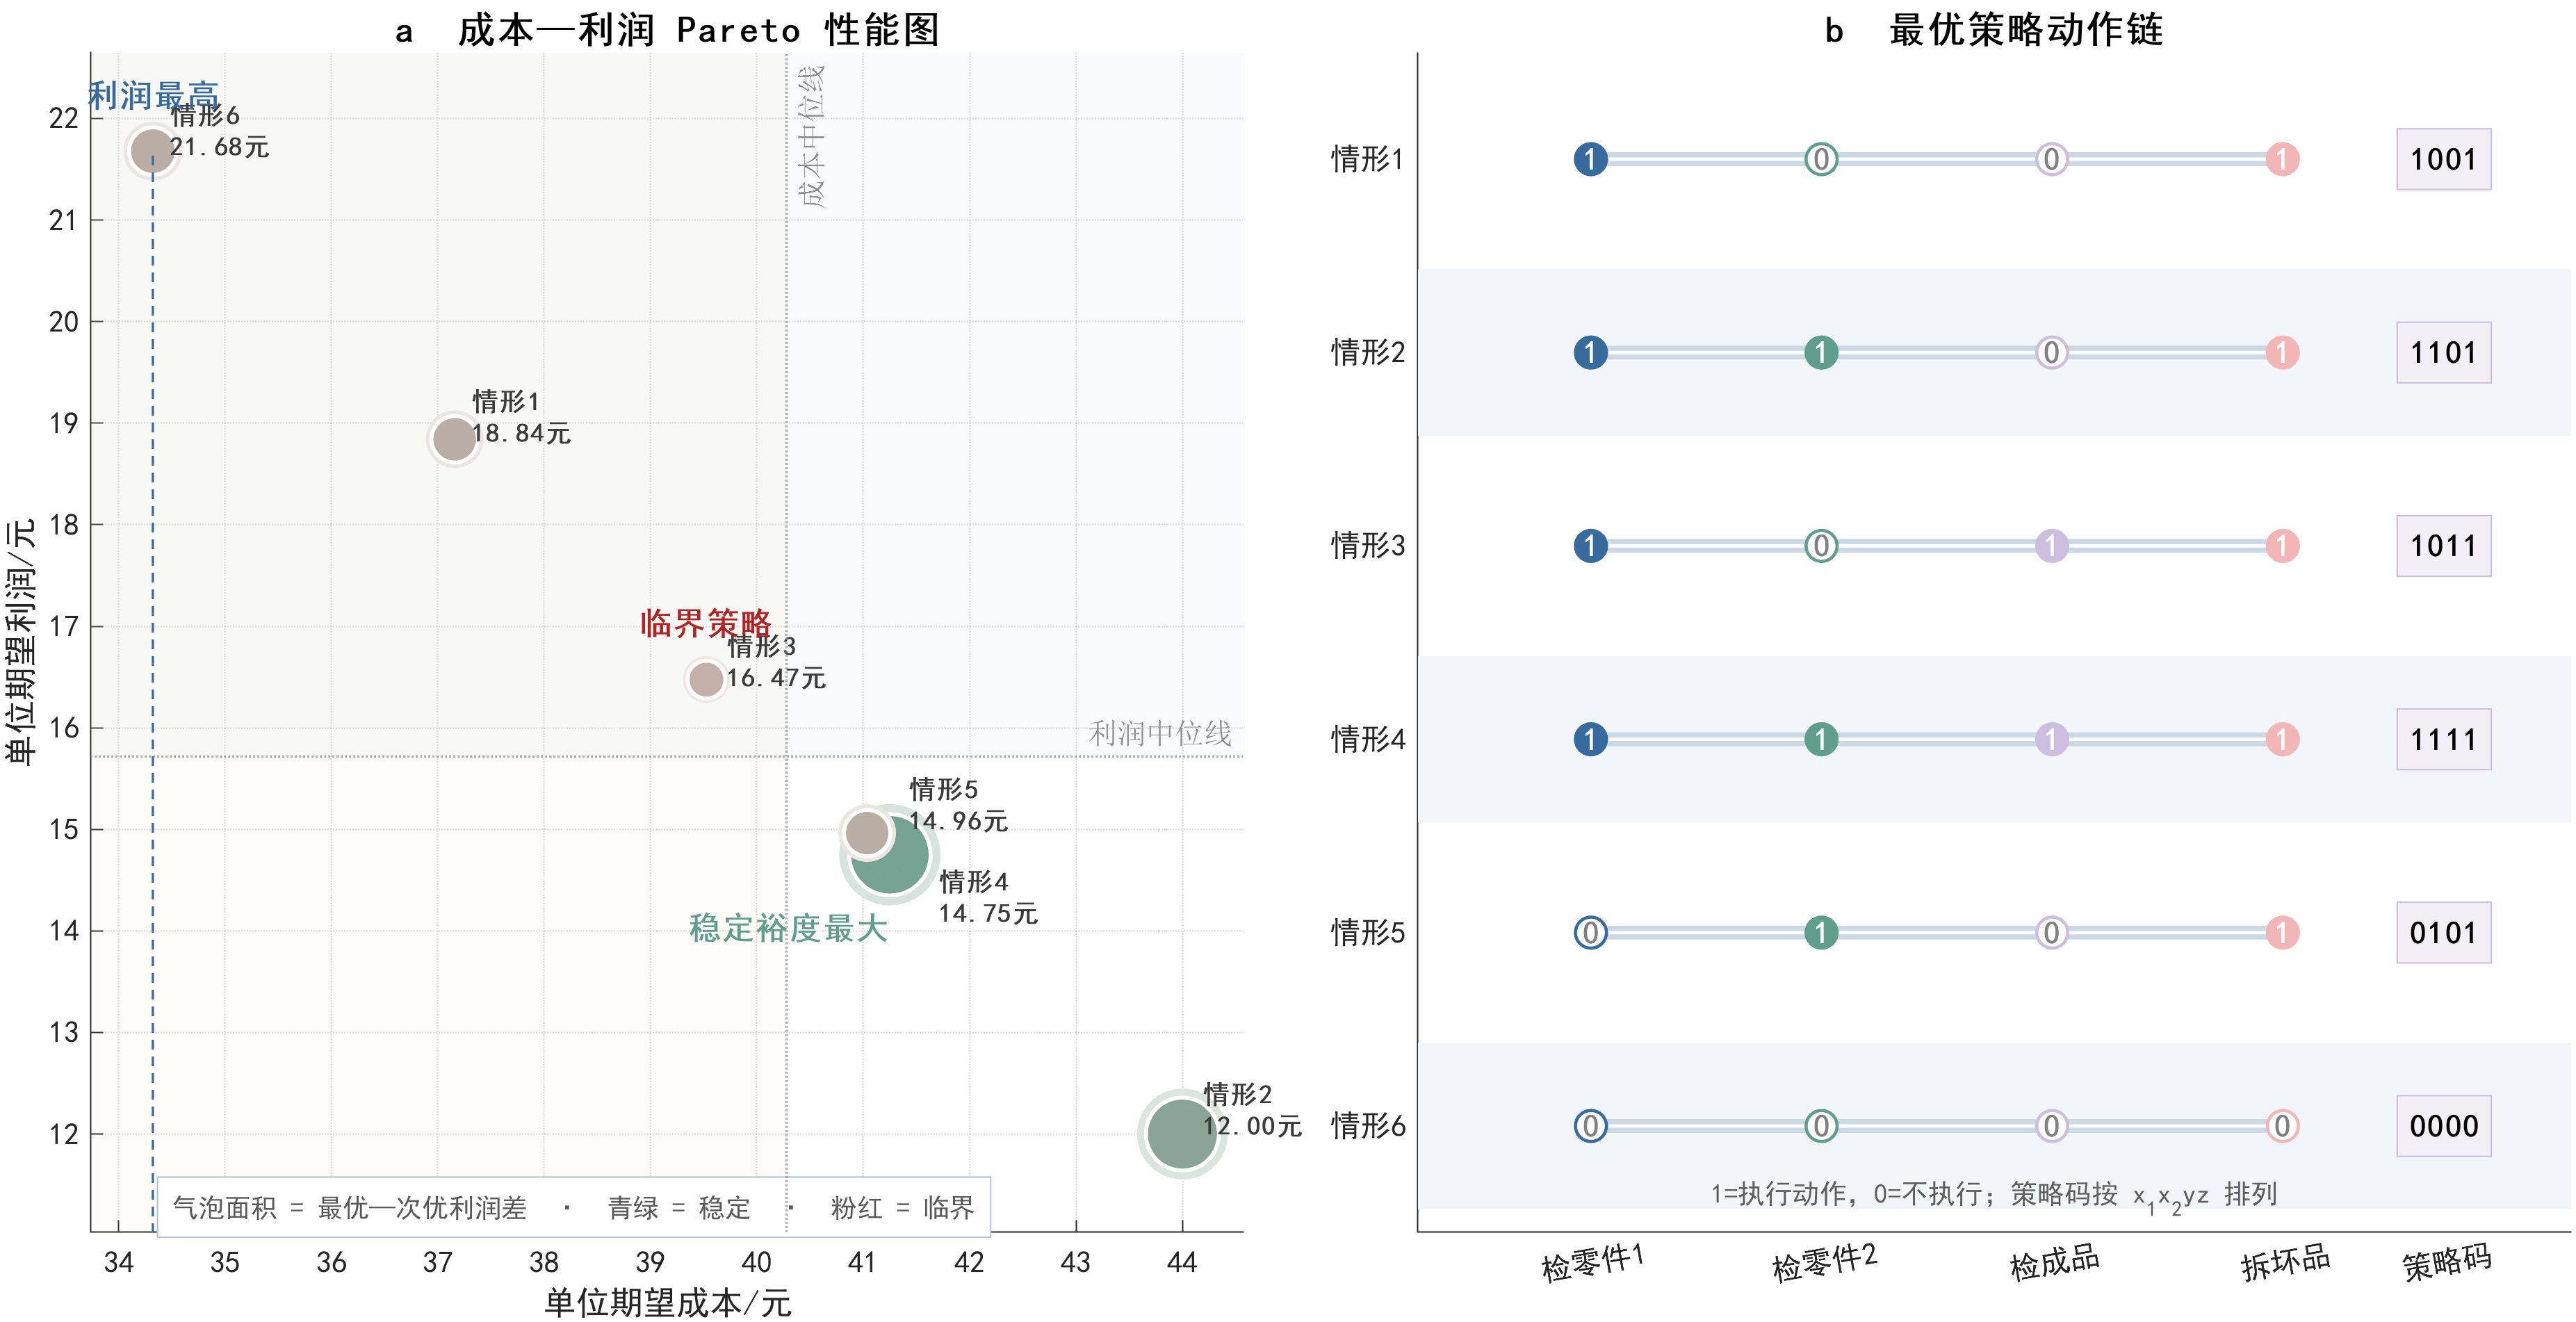
\includegraphics[width=0.95\textwidth]{figures/Q2_图2_最优决策与经济结果.png}
    \caption{六种生产情形最优决策的成本—利润表现与策略结构}
    \label{fig:q2-fig2}
\end{figure}
由图~\ref{fig:q2-fig2}可见，六种情形的最优利润为$12.00$至$21.68$元。情形6成本最低、利润最高，说明低次品率下无需过度检测；情形2因次品率较高，检测投入增加，利润最低。情形4的最优策略优势最明显，而情形3与次优策略利润接近，决策更容易受到参数变化影响。



为深入分析各策略的经济结构，图~\ref{fig:q2-fig3}给出六种情形下的单位期望成本构成及利润空间。




\begin{figure}[H]
    \centering
    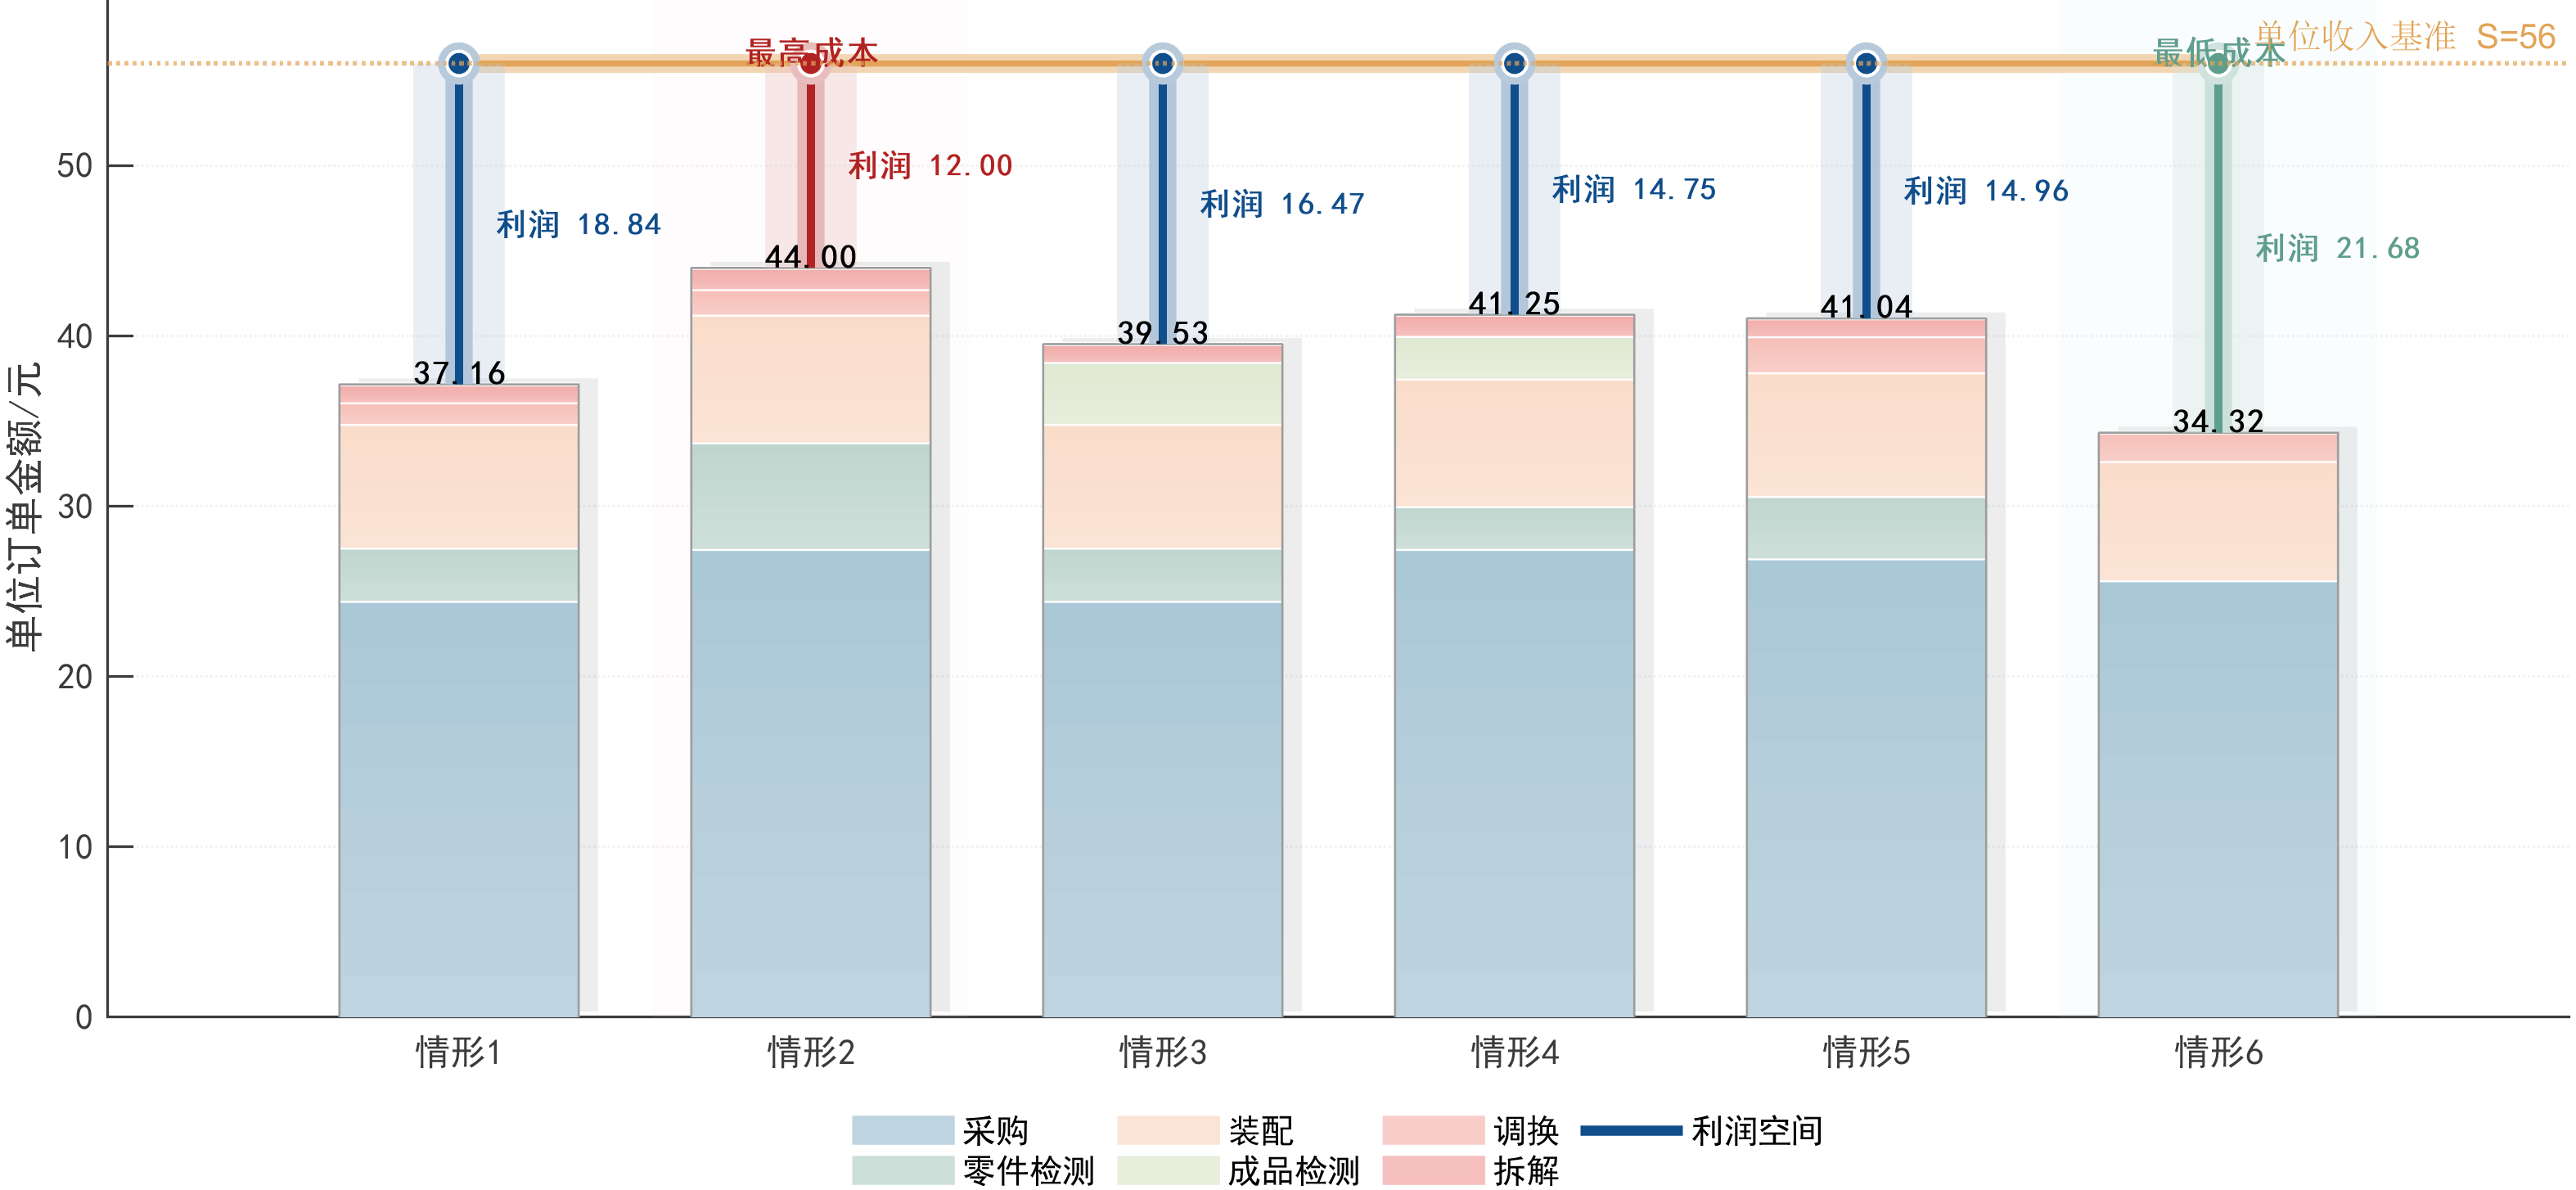
\includegraphics[width=0.95\textwidth]{figures/Q2_图3_最优策略成本构成.png}
    \caption{六种情形最优策略的单位期望成本构成及利润空间}
    \label{fig:q2-fig3}
\end{figure}

    由图可见，各情形的期望成本均以采购成本为主，成品检测能够减少调换损失；情形6总成本最低、利润空间最大，说明在低次品率下过度检测和拆解并不经济。


\subsubsection{问题二的模型检验与结果分析}

为验证模型求解的正确性与可靠性，本文从解析退化、蒙特卡洛模拟及极端情形三个维度进行交叉检验。

\textbf{（1）解析退化验证}

将模型退化为无拆解、无循环情形，并与封闭解析式比较。六种情形共96个策略均通过验证，最大相对误差仅为$5.119\times10^{-16}$，表明模型计算正确。


\textbf{（2）蒙特卡洛模拟验证}

对每种情形随机生成十万笔订单，真实模拟零件好坏、装配成败、客户退换与拆解回收全过程，统计模拟平均利润并与理论期望利润比较。结果如表~\ref{tab:q2-mc}所示。

\begin{figure}[H]
    \centering
    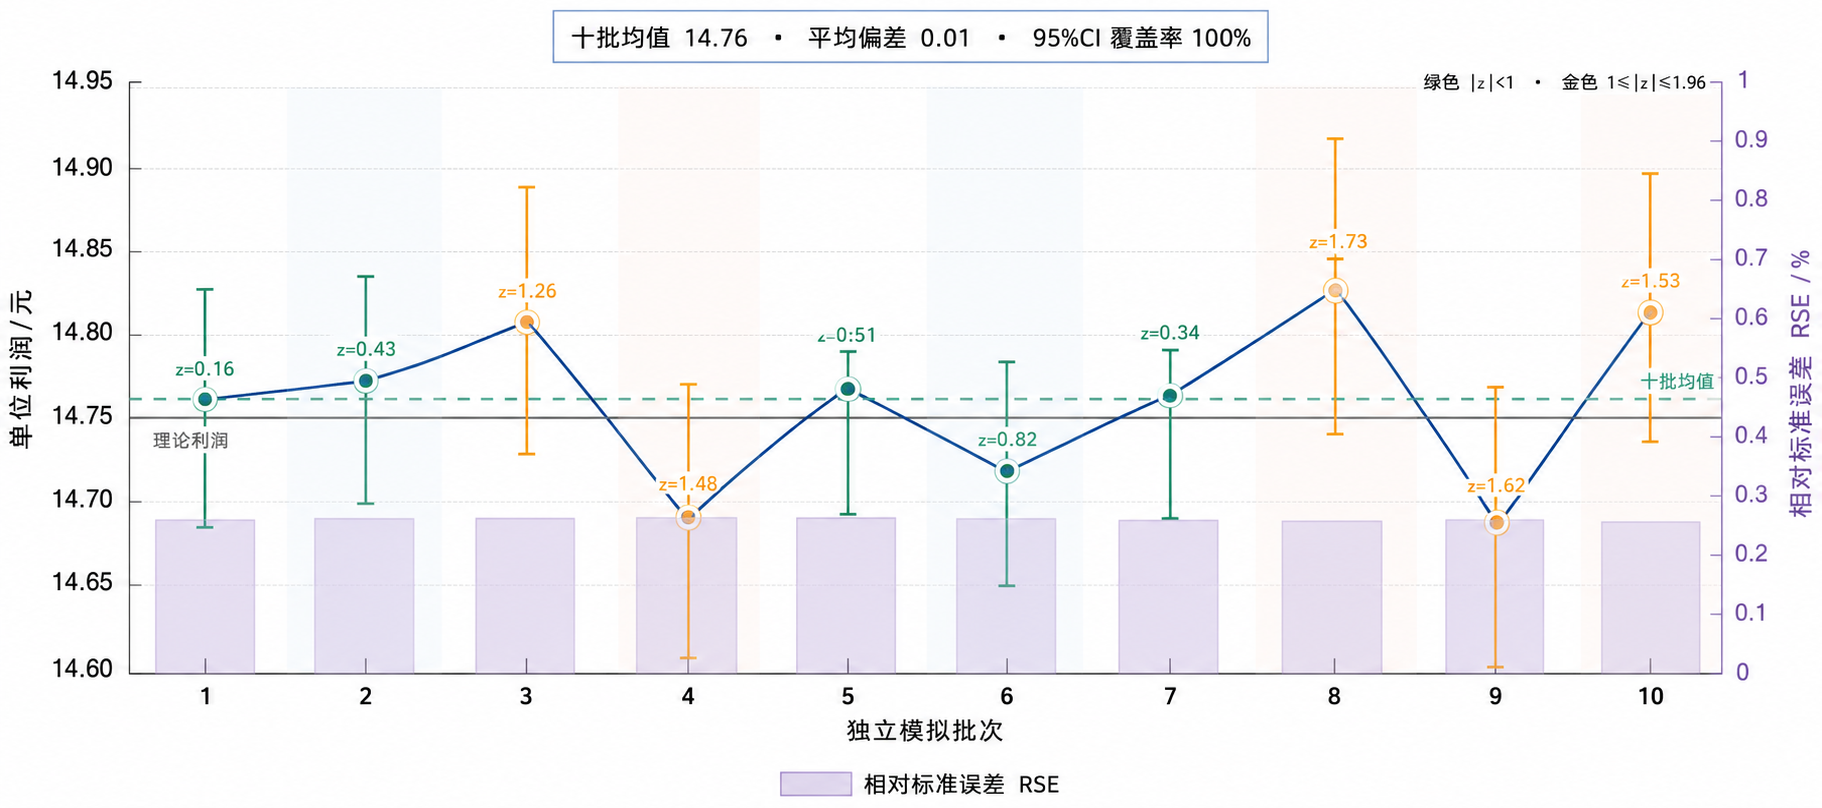
\includegraphics[width=0.95\textwidth]{figures/Q2_附图B_MC多批次验证.png}
    \caption{情形4理论利润的 Monte Carlo 多批次验证结果}
    \label{fig:q2-figB}
\end{figure}


除情形4外，其余情形的理论利润均落入模拟结果的$95\%$置信区间内。情形4因高次品率$20\%$与高调换损失30元并存，次品流出属于小概率稀有事件，蒙特卡洛对稀有路径的采样精度受限，模拟均值(14.87)与理论值(14.75)偏差约0.12元，属正常随机波动范围，不改变该情形的策略结论。



\textbf{（3）极端情形检验}

构造若干极端参数场景检验模型行为，结果如表~\ref{tab:q2-extreme}所示。

\begin{longtable}{>{\centering\arraybackslash}p{0.34\textwidth}>{\centering\arraybackslash}p{0.28\textwidth}>{\centering\arraybackslash}p{0.28\textwidth}}
\caption{极端情形检验结果}
\label{tab:q2-extreme}\\
\toprule[1.5pt]
检验场景 & 理论预期 & 模型输出 \\
\midrule[1pt]
\endfirsthead
\multicolumn{3}{c}{\tablename~\thetable{}（续表）} \\
\midrule[1pt]
检验场景 & 理论预期 & 模型输出 \\
\midrule[1pt]
\endhead
\bottomrule[1.5pt]
\endfoot
\bottomrule[1.5pt]
\endlastfoot
零缺陷且检测费$>0$ & 全不检 & 0000（全不检） \\
调换损失极高 & 检测成品 & 1011（检成品） \\
拆解费用极高 & 不拆解、报废 & 1000（报废） \\
高风险且检测免费 & 全检 & 1111（全检） \\
未知坏回收件永不检测 & 永久循环、不可行 & 不可行（$\rho=1$） \\
\end{longtable}

此外，当两零配件均已证合格时，单轮装配的成品合格率应恰为$1-p_3=0.90$，模型输出与实际一致；而未知坏回收件永不检测的策略因其暂态矩阵谱半径$\rho\geq1$、存在期望成本发散的永久循环，被判定为不可行。

综合三项检验可见，模型在解析退化、蒙特卡洛模拟、极端情形检验中均表现良好，求解结果可靠，可为企业生产决策提供依据。

\textbf{（4）灵敏度分析}

以基准情形1为例，对关键参数进行一维扫描，考察最优策略随参数变化的临界切换点，结果如表~\ref{tab:q2-sensitivity}所示。

\begin{table}[H]
\centering
\caption{情形1关键参数的灵敏度临界值}
\label{tab:q2-sensitivity}
\small
\renewcommand{\arraystretch}{1.2}
\begin{tabularx}{\textwidth}{>{\centering\arraybackslash}p{0.18\textwidth} >{\centering\arraybackslash}p{0.12\textwidth} >{\centering\arraybackslash}p{0.13\textwidth} >{\centering\arraybackslash}p{0.13\textwidth} >{\raggedright\arraybackslash}p{0.30\textwidth}}
\toprule[1.5pt]
参数 & 临界值 & 临界前策略 & 临界后策略 & 当前参数下的结论 \\
\midrule[1pt]
零件1次品率 $p_1$ & $8.37\%$ & 0001 & 1001 & $p_1=10\%>8.37\%$，检测件1 \\
零件2次品率 $p_2$ & $13.71\%$ & 1001 & 1101 & $p_2=10\%<13.71\%$，不检测件2 \\
零件1检测成本 $b_1$ & 2.43 & 1001 & 0001 & $b_1=2<2.43$，检测件1 \\
零件2检测成本 $b_2$ & 2.10 & 1101 & 1001 & $b_2=3>2.10$，不检测件2 \\
调换损失 $L$ & 13.30 & 1001 & 1101 & $L=6<13.30$，不检测成品 \\
拆解成本 $d$ & 12.30 & 1001 & 1101 & $d=5<12.30$，选择拆解 \\
\bottomrule[1.5pt]
\end{tabularx}
\normalsize
\end{table}

当前参数下，零件1次品率$p_1=10\%$高于临界值$8.37\%$，故值得检测零件1；零件2次品率$p_2=10\%$低于临界值$13.71\%$，故不值得检测零件2；调换损失$L=6$低于临界值13.3，故无需检测成品。各临界结论与表~\ref{tab:q2-optimal}得到的最优策略完全一致，再次验证了解的合理性。


\begin{figure}[H]
    \centering
    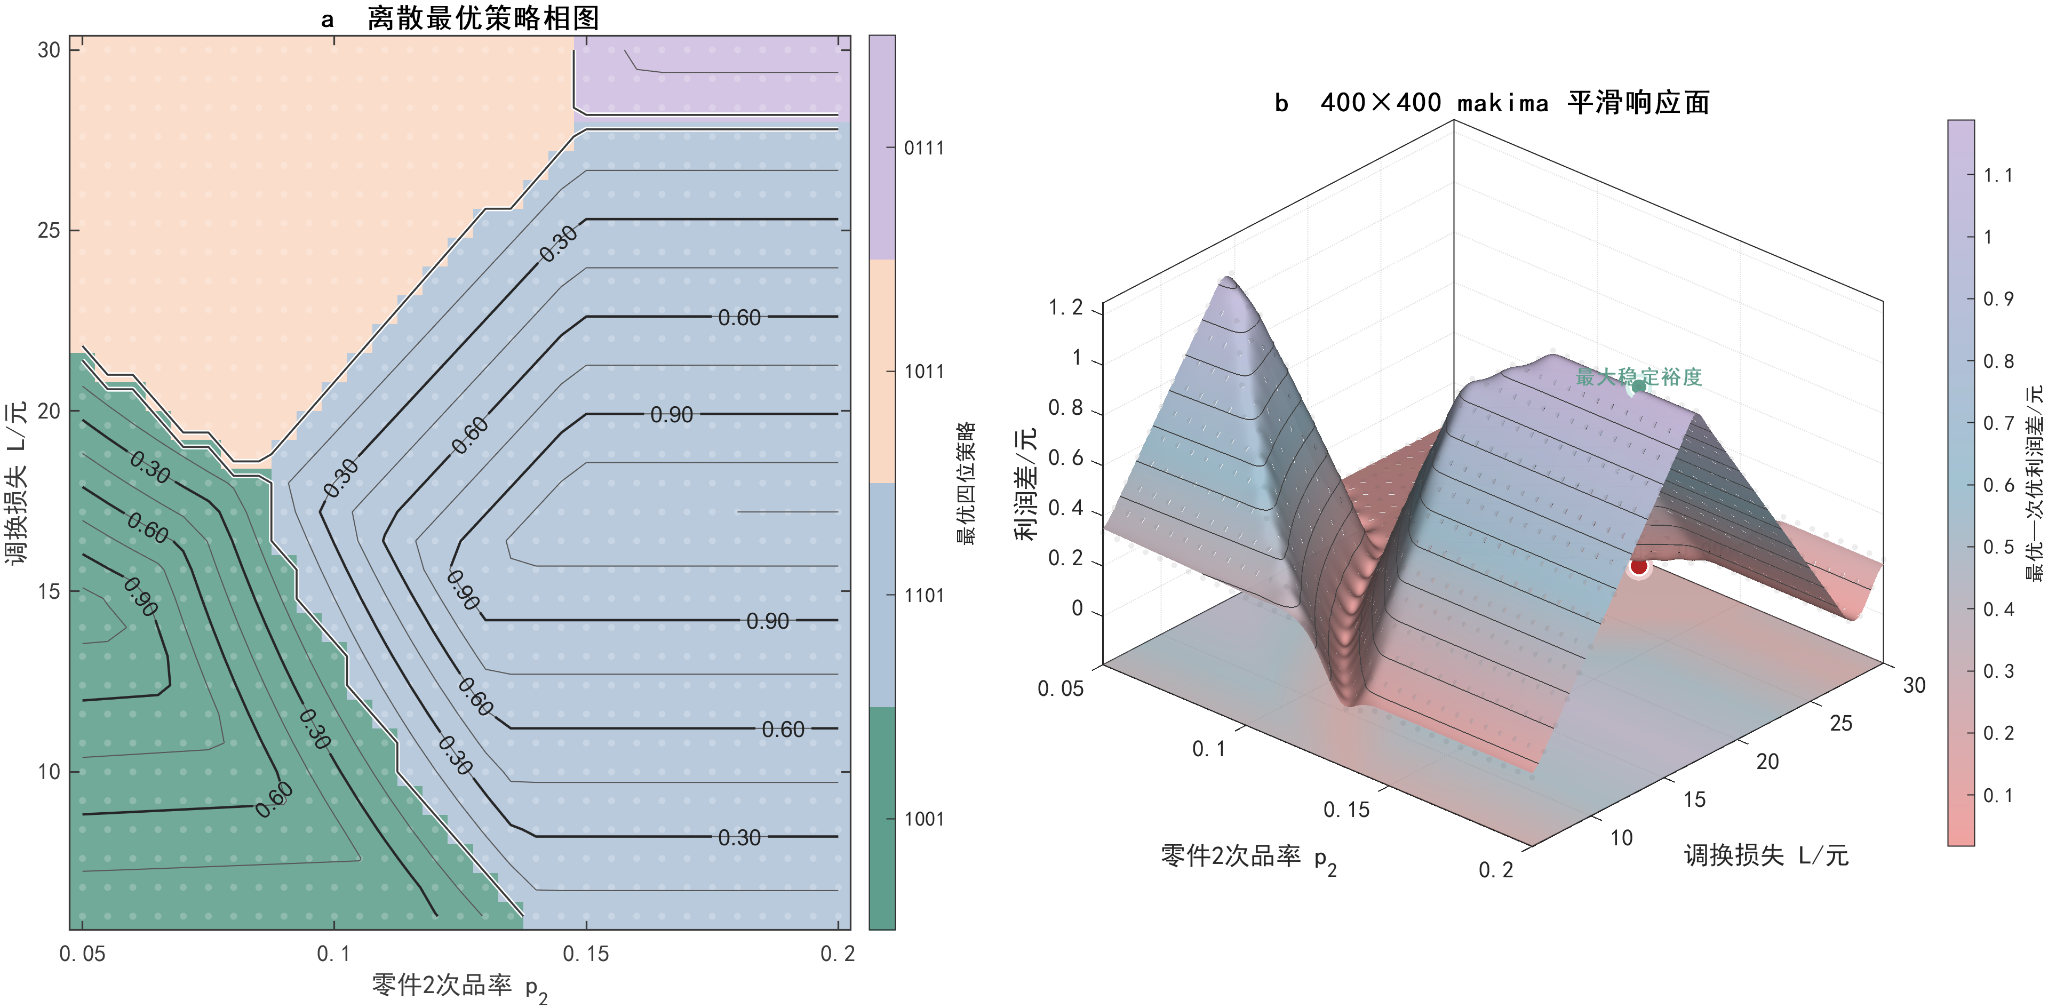
\includegraphics[width=0.95\textwidth]{figures/Q2_图4_策略相图与稳定性.png}
    \caption{情形1中零件2次品率与调换损失共同作用下的策略分区及稳定裕度}
    \label{fig:q2-fig4}
\end{figure}

图~\ref{fig:q2-fig4}~表明，零件2次品率与调换损失$L$的变化会共同推动最优策略切换；在策略分界线附近，利润差较小，决策对参数误差更为敏感。

\begin{figure}[H]
    \centering
    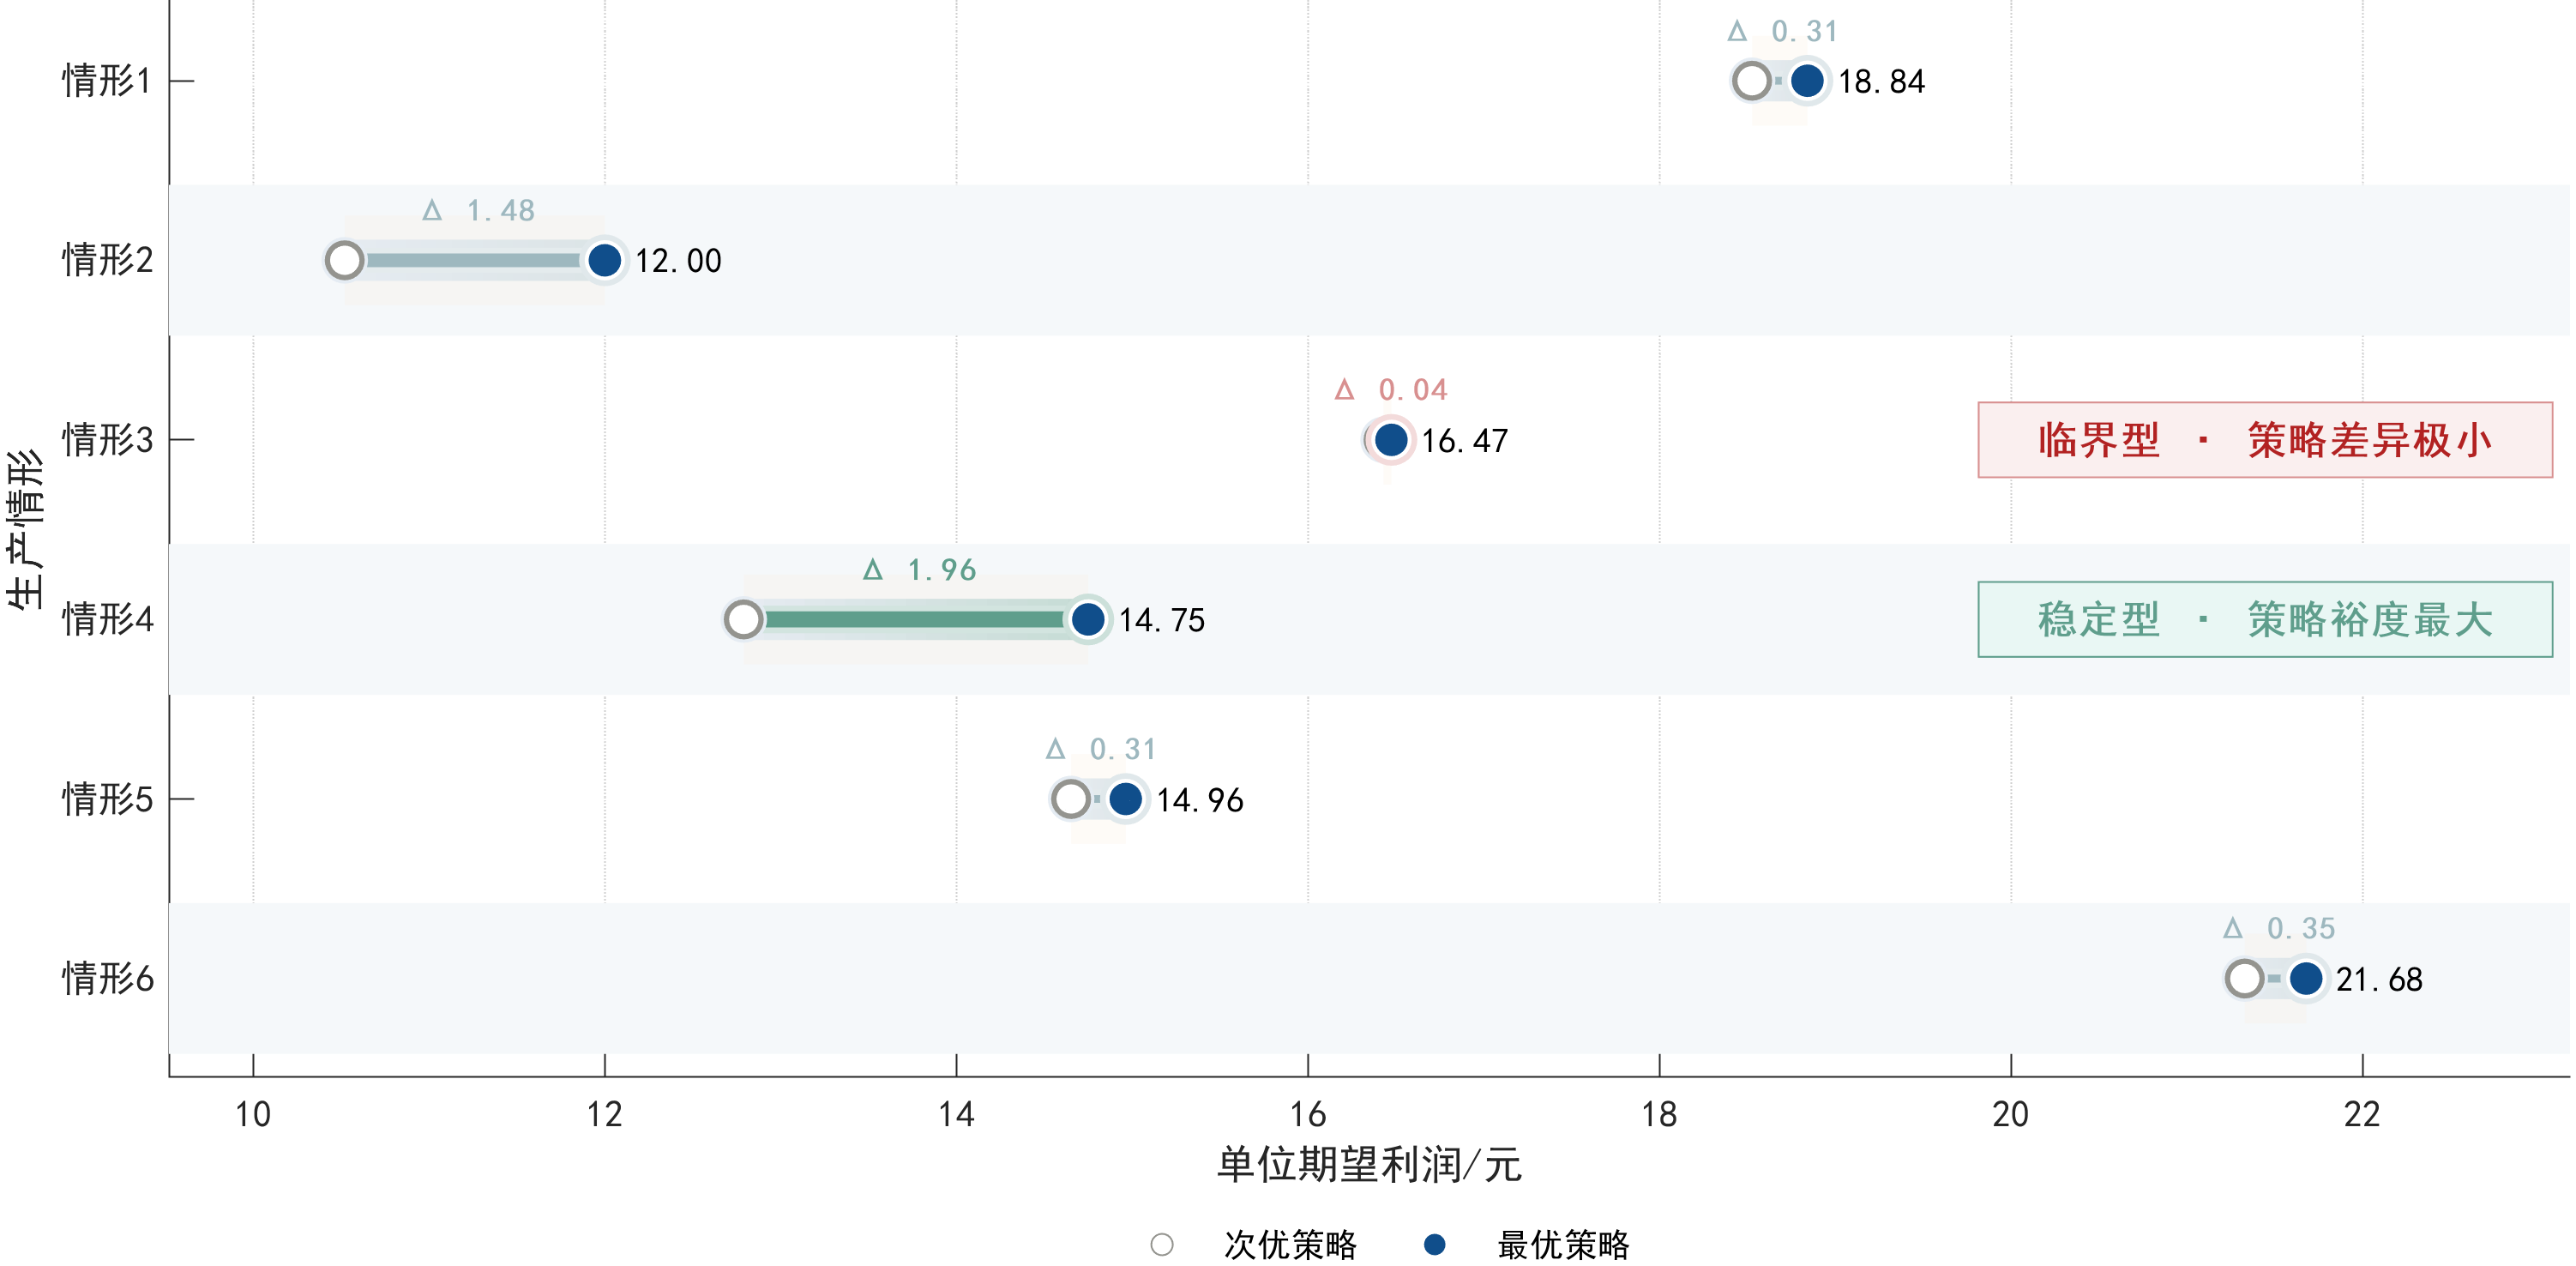
\includegraphics[width=0.95\textwidth]{figures/Q2_图5_最优次优利润比较.png}
    \caption{六种情形最优与次优策略的单位期望利润比较}
    \label{fig:q2-fig5}
\end{figure}

图~\ref{fig:q2-fig5}~进一步比较六种情形最优策略与次优策略的单位期望利润。六种情形的利润差依次为0.31、1.48、0.04、1.96、0.31、0.35元。其中情形4的利润差最大，策略1111相对次优策略具有较清晰的优势；情形3的利润差最小，最优策略1011与次优策略0011在经济表现上几乎相当，属于临界情形，对情形3给出确定性策略结论时应附带临界性说明。

\begin{figure}[H]
    \centering
    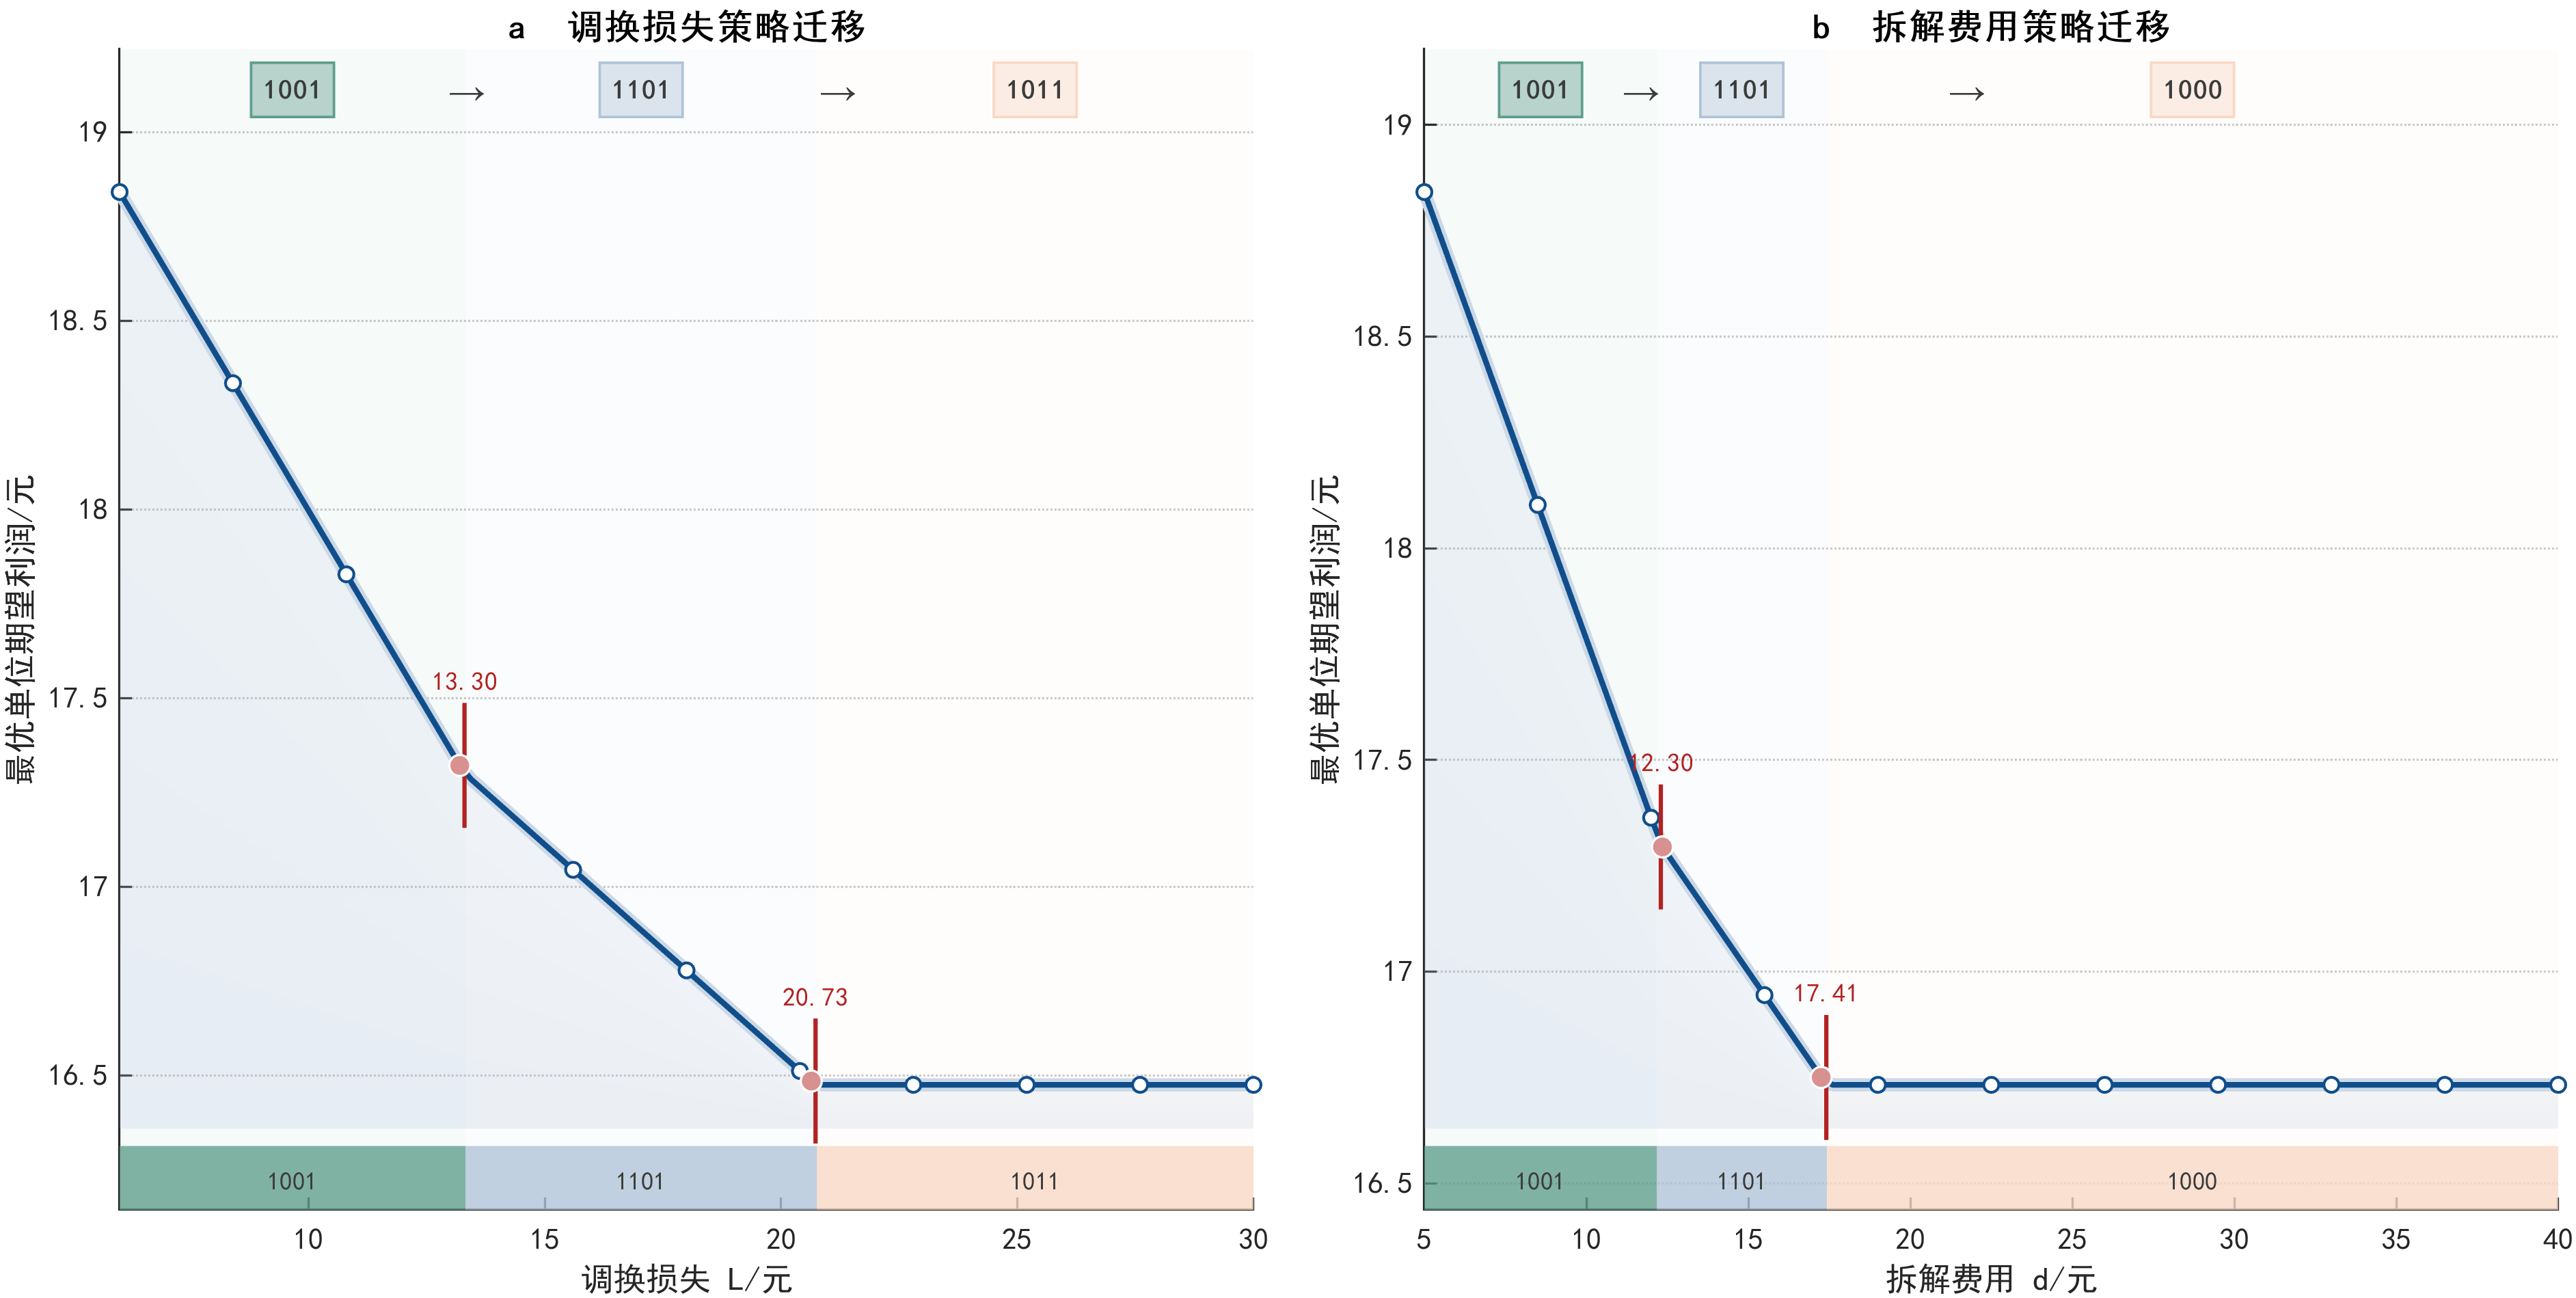
\includegraphics[width=0.95\textwidth]{figures/Q2_附图A_单参数策略切换.png}
    \caption{情形1中调换损失与拆解费用变化下的最优策略切换}
    \label{fig:q2-figA}
\end{figure}




图~\ref{fig:q2-figA}~展示单参数变化下的策略迁移。当调换损失 $L$ 增加时，最优策略依次发生1001$\rightarrow$1101$\rightarrow$1011的迁移，对应阈值约13.30元和20.73元；当拆解费用增加时，策略在12.30元附近由1001切换为1101，并在17.41元附近进一步切换为1000，反映出拆解回收价值下降后继续拆解不再划算。在两处临界阈值附近，两侧策略利润近似相等，实际应用时应在阈值附近设置缓冲区，避免参数轻微波动造成频繁切换。





\subsubsection{问题二的结论}
针对问题二，本文得到的六种情形最优方案如表~\ref{tab:q2-optimal}所示。


通过模型检验与灵敏度分析，验证了本文模型具有较好的稳定性。















\subsection{问题三的模型建立与求解}












\subsubsection{问题三的模型建立}
问题三的生产系统包含八种零配件、三个半成品和一个成品,其装配关系如图~\ref{fig:assembly-structure}所示。与问题二的单层闭环不同,本题的决策需沿 BOM 树形结构逐层展开。

\textbf{1. 多层级检测与拆解决策模型的建立}

题目共涉及 16 个 0-1 决策变量。
首先,在零配件进入装配环节前,企业需决定是否对每种零配件进行检测。令
\begin{equation}
x_i=
\begin{cases}
1, & \text{检测零配件 }i\\
0, & \text{不检测零配件 }i
\end{cases}
\qquad i=1,2,\dots,8
\end{equation}

半成品装配完成后,企业需决定是否对其进行检测。令
\begin{equation}
y_j=
\begin{cases}
1, & \text{检测半成品 }j\\
0, & \text{不检测半成品 }j
\end{cases}
\qquad j=1,2,3
\end{equation}

对于检测或售后过程中发现的不合格半成品,企业需决定是直接报废还是拆解回收其中的零配件。令
\begin{equation}
z_j=
\begin{cases}
1, & \text{拆解不合格半成品 }j\\
0, & \text{直接报废该半成品}
\end{cases}
\qquad j=1,2,3
\end{equation}

在成品层面,企业需决定是否对其进行检测,以及不合格成品是否拆解。令
\begin{equation}
y_{\text{f}}=
\begin{cases}
1, & \text{检测成品}\\
0, & \text{不检测成品}
\end{cases}
\qquad
z_{\text{f}}=
\begin{cases}
1, & \text{拆解不合格成品}\\
0, & \text{直接报废}
\end{cases}
\end{equation}

综上,一个完整策略由 16 个二元变量构成,编码为
\begin{equation}
\boldsymbol{x}=(x_1,\dots,x_8,y_1,y_2,y_3,z_1,z_2,z_3,y_{\text{f}},z_{\text{f}})
\end{equation}

总策略空间为 $2^{16}=65536$ 种方案。

\textbf{2. 分层质量状态摘要递推模型的建立}

本问题的完整决策周期仍然以企业最终成功交付一件合格成品为口径,期望利润为市场售价减去期望总成本。

问题三具有明显的BOM层级结构，若展开所有节点状态，模型复杂度会迅速增加。因此，本文采用分层状态压缩递推方法，将各子树的成本、质量等关键信息汇总后传递至上层。其网络拓扑与状态递推框架如图~\ref{fig:q3-bom}所示。

\begin{figure}[H]
    \centering
    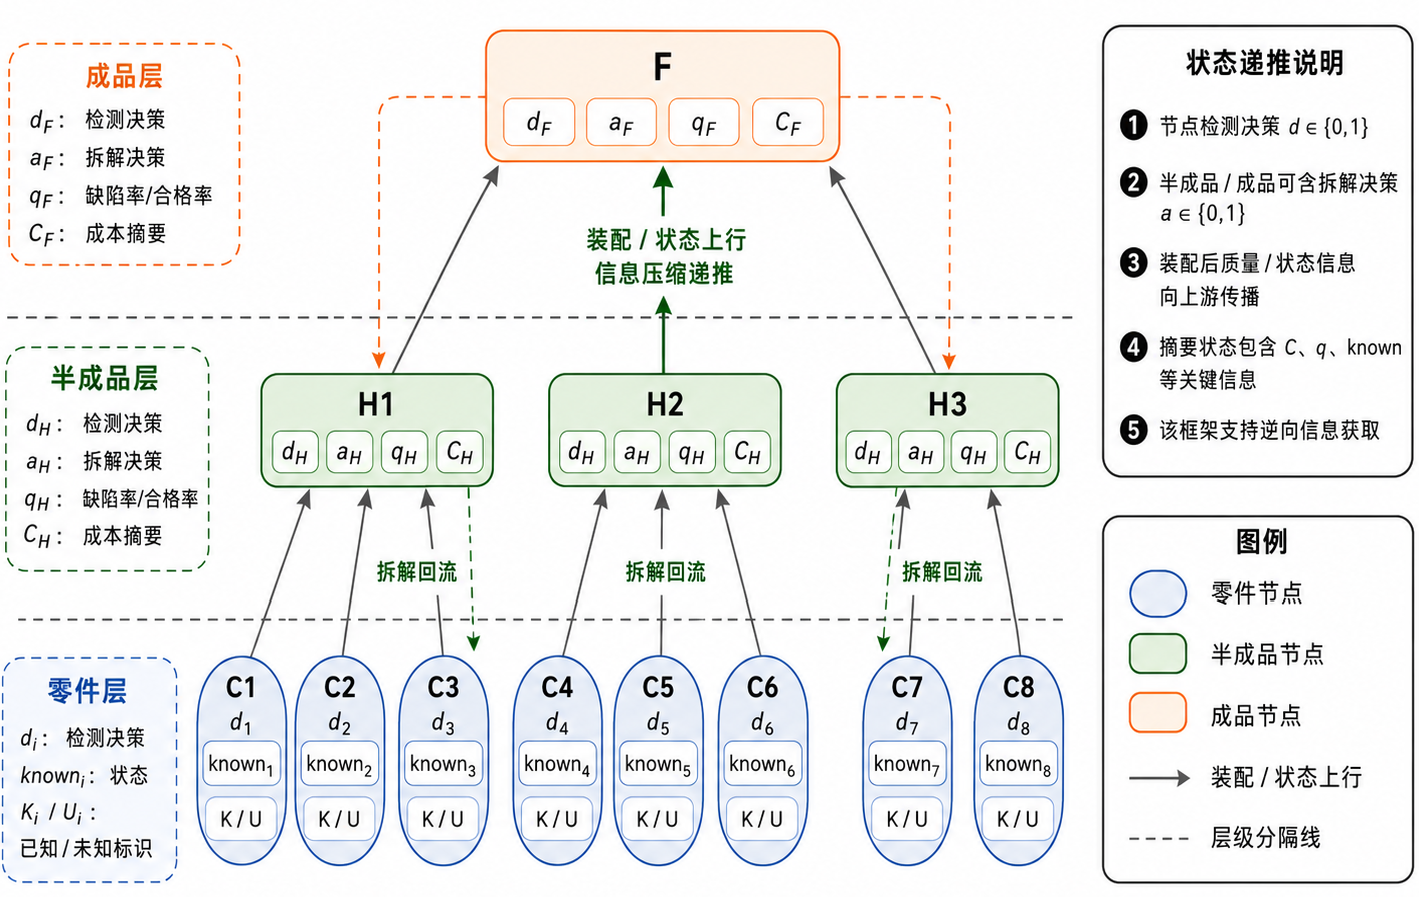
\includegraphics[width=0.85\textwidth]{figures/q3_fig1_bom.png}
    \caption{BOM 网络拓扑与状态递推框架}
    \label{fig:q3-bom}
\end{figure}

图中八类零配件 $C_1$—$C_8$ 分别进入三个半成品 $H_1$—$H_3$，随后共同装配为成品 $F$。每个节点同时记录质量状态与成本状态：完成检测后质量由未知转为已知，发现不合格品时可选择报废或拆解；拆解得到的未知回收件则依据上级产品已失败这一信息，通过贝叶斯条件概率更新其良品概率，再返回相应装配环节。
定义每个节点的状态描述为
\begin{equation}
\mathcal{D}=(C,q,\ell,K,D,b)
\end{equation}
其中：$C$ 为按当前策略获得一个该节点输出的期望成本；$q$ 为该输出为合格品的概率；$\ell$ 为企业是否已确认该节点必然合格；$K$ 为从头获得一个已知合格节点的期望成本；$D$ 为节点被确认不合格后修复为已知合格的期望成本；$b$ 为该节点单次检测费用。



\textbf{零配件处理：} 对于基础零件 $i$，令$x_i$表示是否检测，则其期望成本、合格概率和质量信息状态分别为
\begin{equation}
\begin{aligned}
C_i(x_i)&=
\begin{cases}
a_i, & x_i=0,\\[2pt]
\dfrac{a_i+b_i}{1-p_i}, & x_i=1,
\end{cases}
\\[6pt]
q_i(x_i)&=
\begin{cases}
1-p_i, & x_i=0,\\
1, & x_i=1,
\end{cases}
\\[6pt]
\ell_i(x_i)&=
\begin{cases}
0, & x_i=0,\\
1, & x_i=1.
\end{cases}
\end{aligned}
\end{equation}
其中，$C_i$为获得零件$i$的期望成本，$q_i$为其合格概率，$\ell_i=1$表示该零件已被确认合格，$\ell_i=0$表示其质量仍未知。

\textbf{半成品层处理：} 设半成品$j$的输入集合为$\mathcal{I}_j$，其状态描述为$\{\mathcal{D}_k:k\in\mathcal{I}_j\}$。令$p_j$、$a_j$、$b_j$和$d_j$分别表示工序次品率、装配费、检测费和拆解费，则
\begin{equation}
g_j=(1-p_j)\prod_{k\in\mathcal{I}_j}q_k
\end{equation}
\begin{equation}
B_j=a_j+\sum_{k\in\mathcal{I}_j}C_k
\end{equation}

当$z_j=0$时，半成品报废并重新生产，直至获得已知合格输出：
\begin{equation}
K_j=\frac{B_j+b_j}{g_j}.
\end{equation}

令$H_j$表示半成品$j$合格，$\bar H_j$表示半成品$j$不合格；令$Z_u=1$表示输入$u$合格，$Z_u=0$表示输入$u$不合格。若$z_j=1$，则拆解并更新未知输入的质量概率：
\begin{equation}
r_{u\mid j}=P(Z_u=0\mid\bar H_j)
\end{equation}
\begin{equation}
r_{u\mid j}=\frac{1-q_u}{1-g_j}.
\end{equation}

记回收输入的认证成本为$R_u(r_{u\mid j})$，工序自身失败的循环修复成本为$T_j$，则
\begin{equation}
D_j=d_j+\sum_{u\in\mathcal{I}_j}R_u(r_{u\mid j})+T_j.
\end{equation}

\textbf{成品层处理：} 设最终成品$F$的输入集合为$\mathcal{I}_F$，其状态描述为$\{\mathcal{D}_k:k\in\mathcal{I}_F\}$。令$p_F$、$a_F$、$b_F$和$L$分别表示成品工序次品率、装配费、检测费和调换损失，则
\begin{equation}
g_F=(1-p_F)\prod_{k\in\mathcal{I}_F}q_k,
\qquad
B_F=a_F+\sum_{k\in\mathcal{I}_F}C_k.
\end{equation}

令$K_F$和$D_F$分别表示成品报废和拆解后的恢复成本，则失败后的处理成本为
\begin{equation}
W_F(z_F)=(1-z_F)K_F+z_FD_F.
\end{equation}

将成品检测决策$y_F$、售后调换和失败后的循环统一计入，可得
\begin{equation}
C_F=\frac{B_F+y_Fb_F+(1-g_F)\left[(1-y_F)L+W_F(z_F)\right]}{g_F}.
\end{equation}

相应的期望利润为
\begin{equation}
\pi_F=S-C_F.
\end{equation}

\textbf{3. 全局最优方案的期望利润优化模型的建立}

由于候选策略仅有 $65536$ 种，本文采用全枚举结合 BOM 递推模型计算各方案的期望利润，并选取利润最大的方案作为全局最优解。













\subsubsection{问题三的求解结果}


对问题三的全部 $2^{16}=65536$ 种策略进行全枚举求解，选取期望利润最大的方案作为最优策略。得到的最优策略为 \texttt{1111111111111101}，对应的单位期望成本为 139.78 元，单位期望利润为 60.22 元。最优策略的各层级决策如表~\ref{tab:q3-optimal} 所示。

\begin{table}[H]
\centering
\caption{问题三的最优策略及经济含义}
\label{tab:q3-optimal}
\begin{tabularx}{\textwidth}{>{\centering\arraybackslash}p{0.25\textwidth} >{\centering\arraybackslash}p{0.20\textwidth} >{\raggedright\arraybackslash}p{0.45\textwidth}}
\toprule[1.5pt]
决策层 & 最优取值 & 经济含义 \\
\midrule[1pt]
零配件检测 & 11111111 & 八种零配件全部检测，阻断质量风险向下游传播 \\
半成品检测 & 111 & 三个半成品全部检测，及时截获工序次品 \\
半成品拆解 & 111 & 不合格半成品均拆解，回收合格零配件 \\
成品检测 & 0 & 不做出厂检测，检测边际成本高于可避免损失 \\
成品拆解 & 1 & 退回成品拆解，回收合格半成品 \\
\bottomrule[1.5pt]
\end{tabularx}
\end{table}

该结果呈现出差异化策略：零配件和半成品检测能够在风险进入下游前将其截获，且拆解可回收已确认合格的零配件，因此相应决策均取$1$。而三个半成品均合格后，成品层仅剩$10\%$的装配缺陷风险，成品检测可避免的期望调换损失仅为$0.1\times40=4$元，小于$6$元的检测费用，故最优策略选择成品不检、退回后拆解。这表明检测应优先布置在能阻断后续损失的关键层级，而不是对所有产品进行盲目全检。

将最优策略的 16 个二元决策映射回 BOM 节点，得到可执行的最优检测—拆解决策网络，如图~\ref{fig:q3-policy}所示。

\begin{figure}[H]
    \centering
    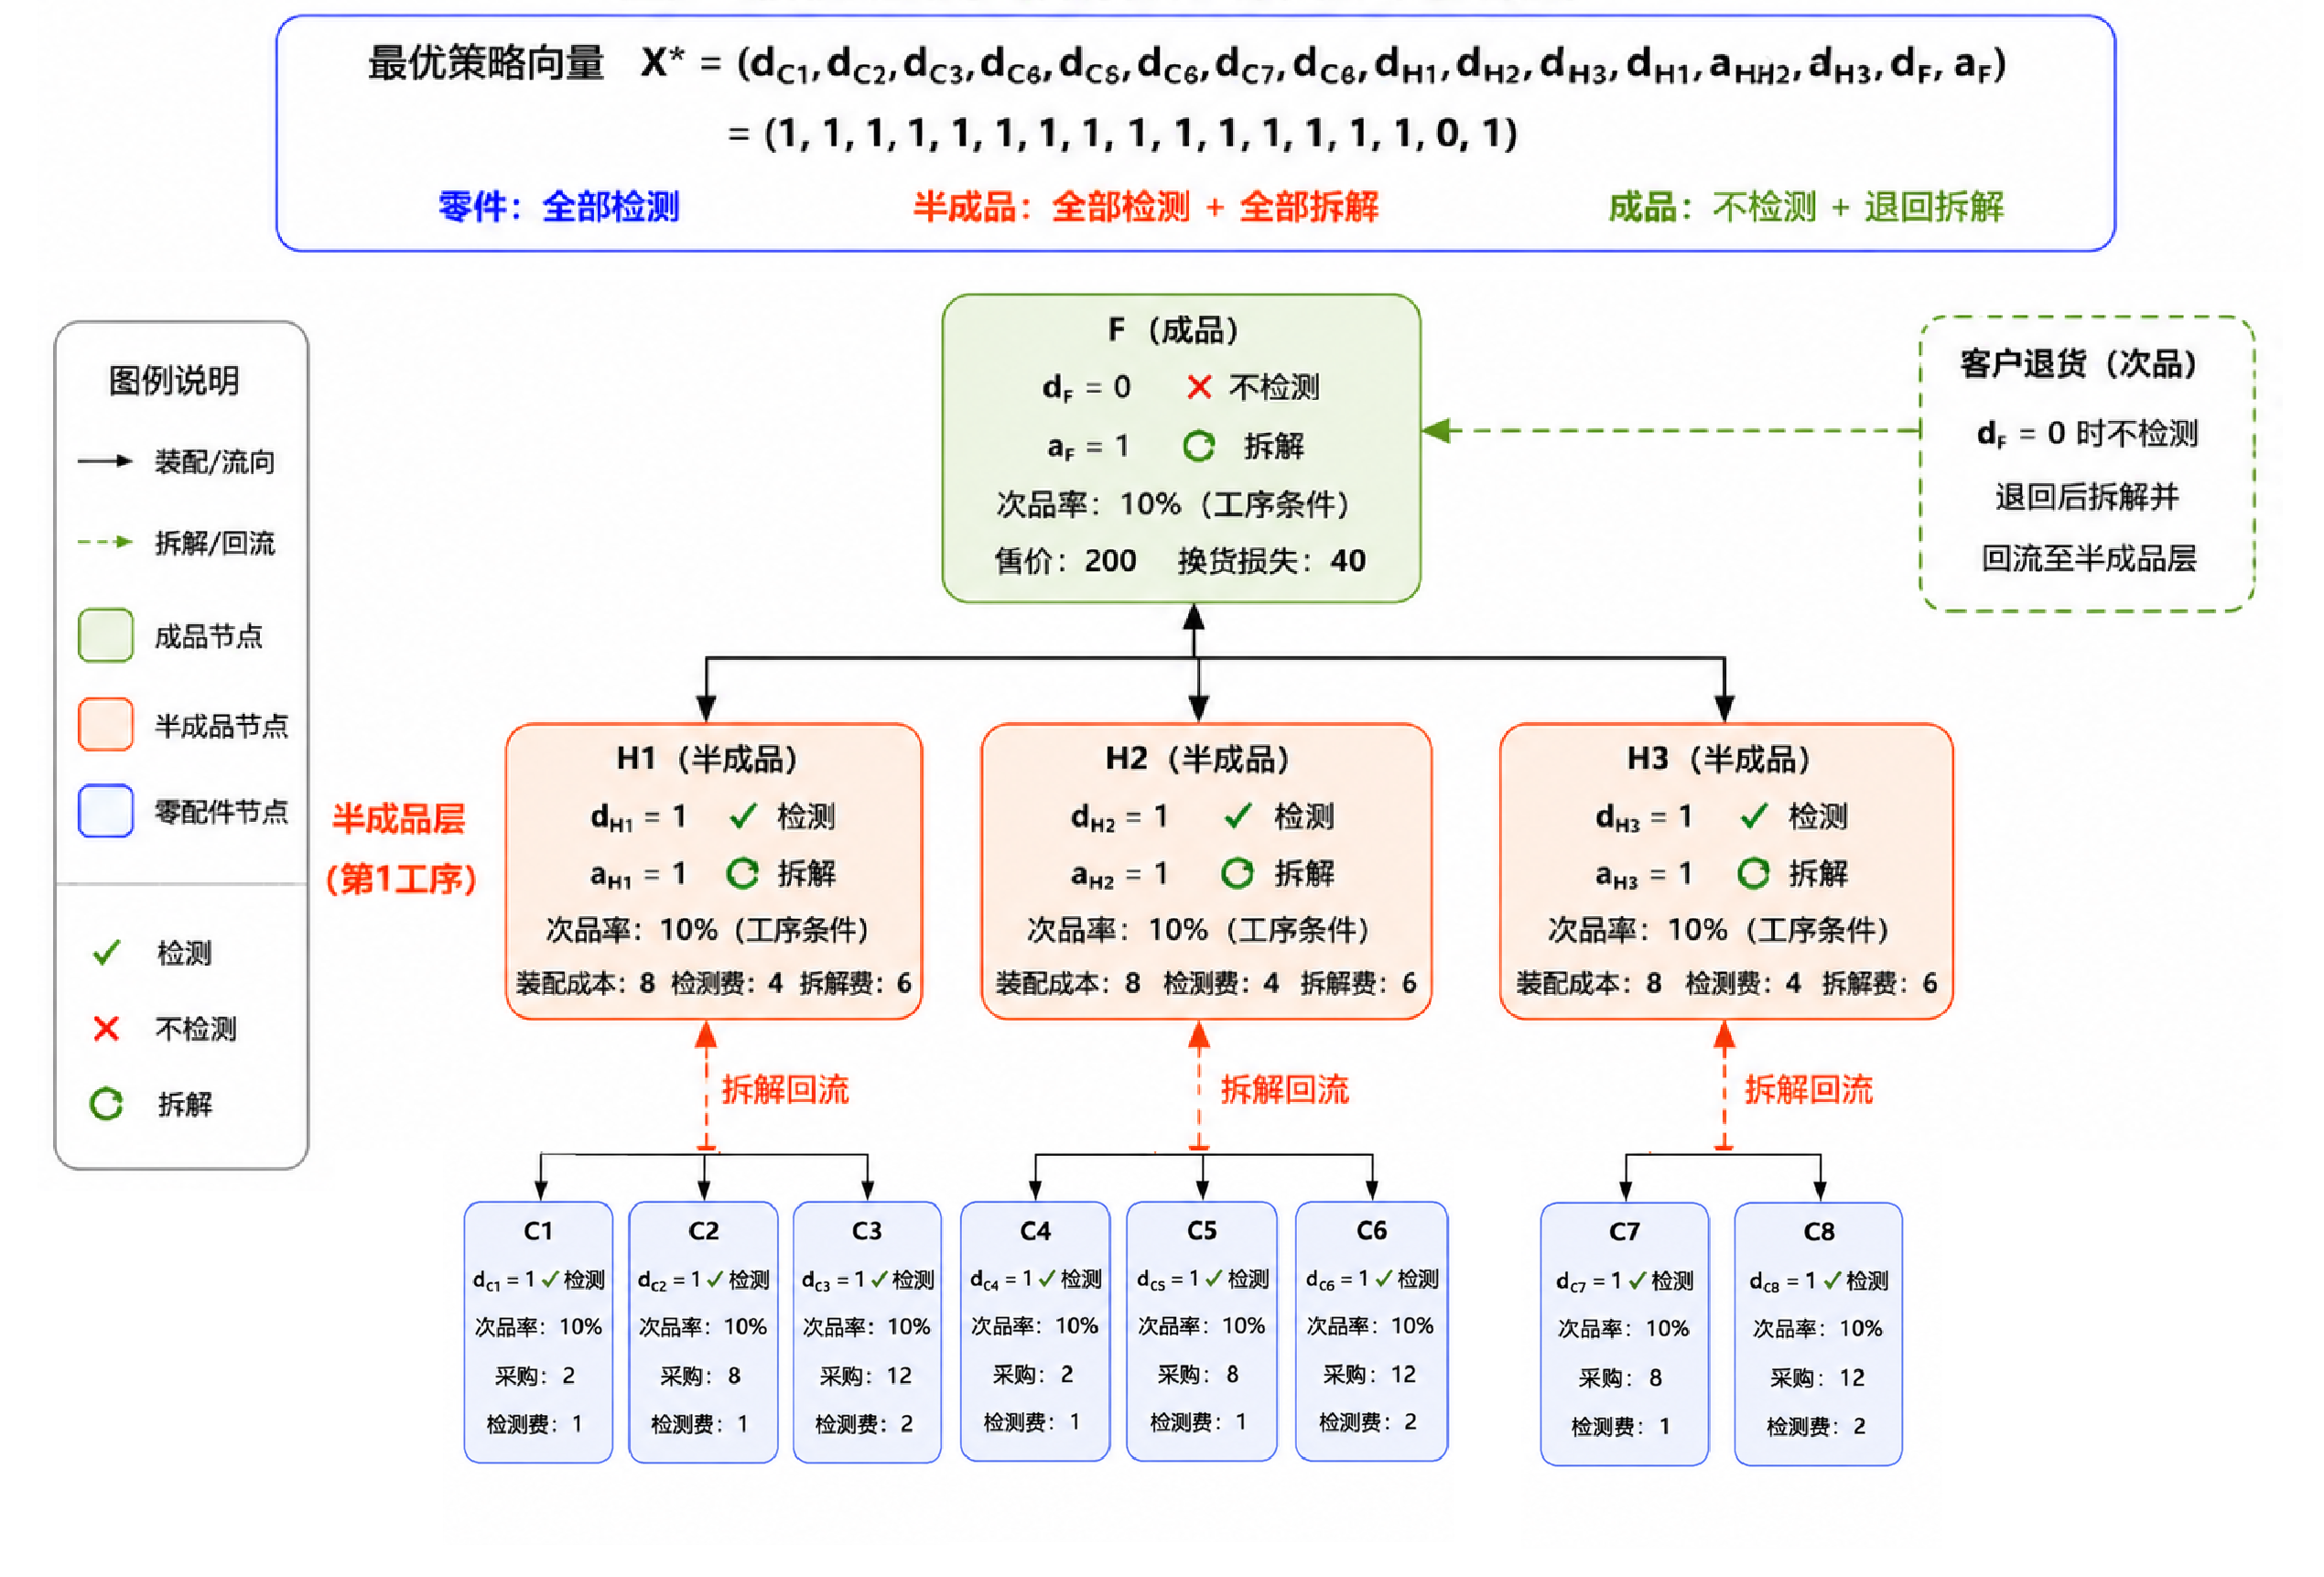
\includegraphics[width=0.85\textwidth]{figures/q3_fig2_policy.png}
    \caption{最优检测—拆解策略决策图}
    \label{fig:q3-policy}
\end{figure}

在最优策略下，期望总成本为 139.78 元，其成本结构分解如图~\ref{fig:q3-cost}所示。

\begin{figure}[H]
    \centering
    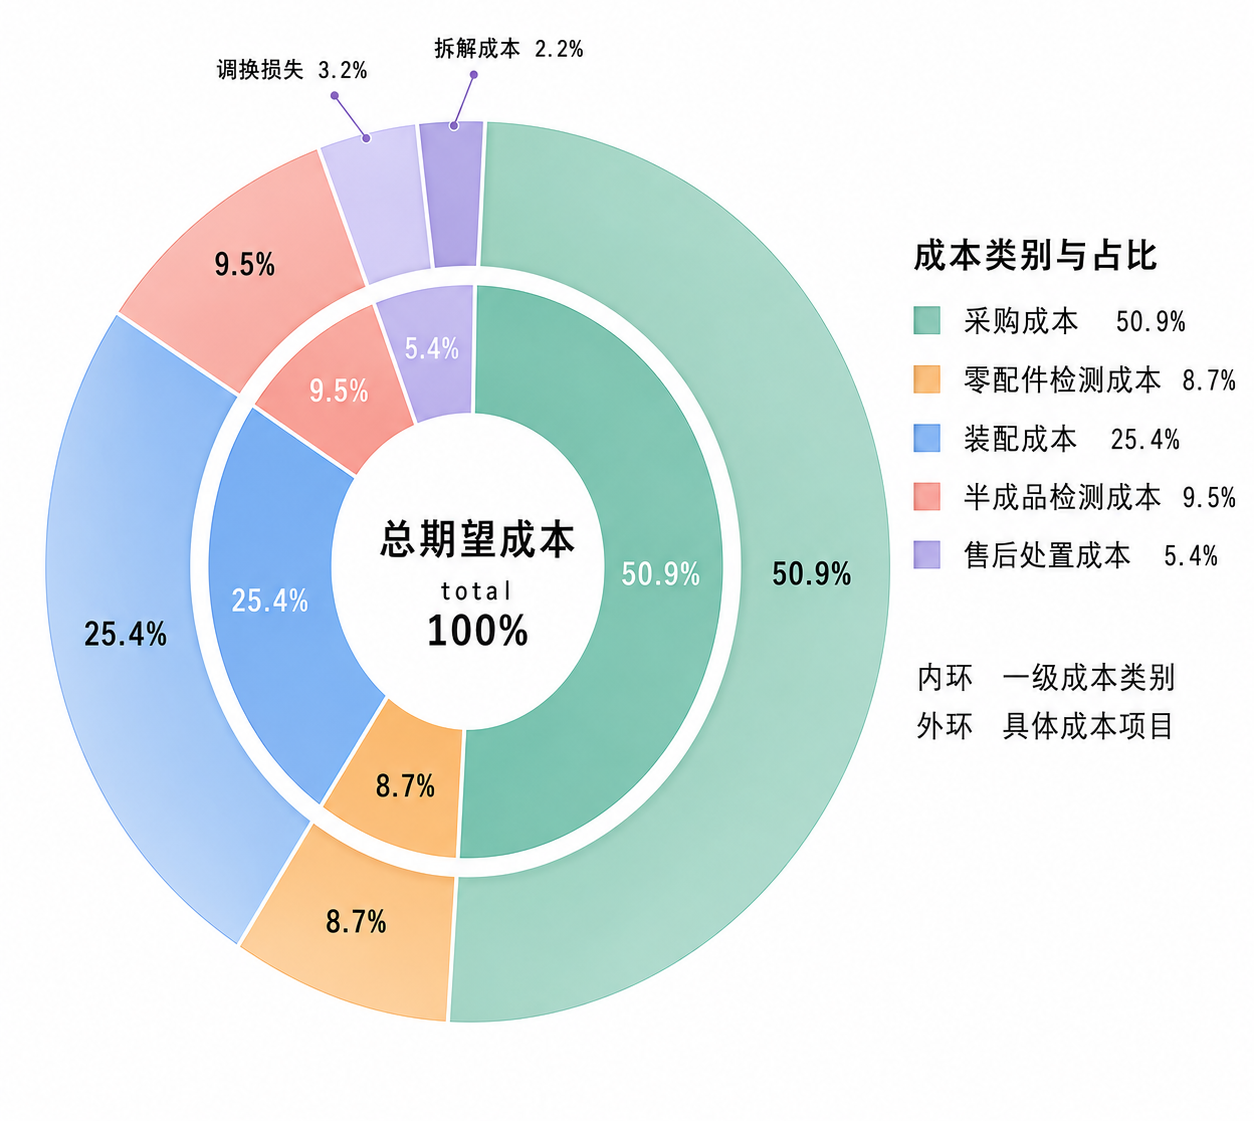
\includegraphics[width=0.5\textwidth]{figures/q3_fig3_cost.png}
    \caption{最优策略下的检测成本结构分解}
    \label{fig:q3-cost}
\end{figure}

其中采购与装配成本合计占 76.31\%，构成成本主体；检测费用约占 18.28\%，以较小的前置投入减少下游装配浪费与调换损失，属于质量控制支出在生产链中的重新配置；调换损失与拆解成本分别占 3.18\% 与 2.23\%，成品检测成本为 0。售价 200 元与总成本之间形成 60.22 元的期望利润空间。



\subsubsection{问题三的模型检验与结果分析}

为验证模型求解的正确性与可靠性，本文从近优策略比较、解析闭式、Monte Carlo 独立模拟、极端情形与灵敏度五个维度进行交叉检验。

\textbf{（1）近优策略比较}

仅报告单一最优解不足以判断方案是否稳健，因此进一步比较期望利润最高的十种策略，如图~\ref{fig:q3-top10}所示。
\begin{figure}[H]
    \centering
    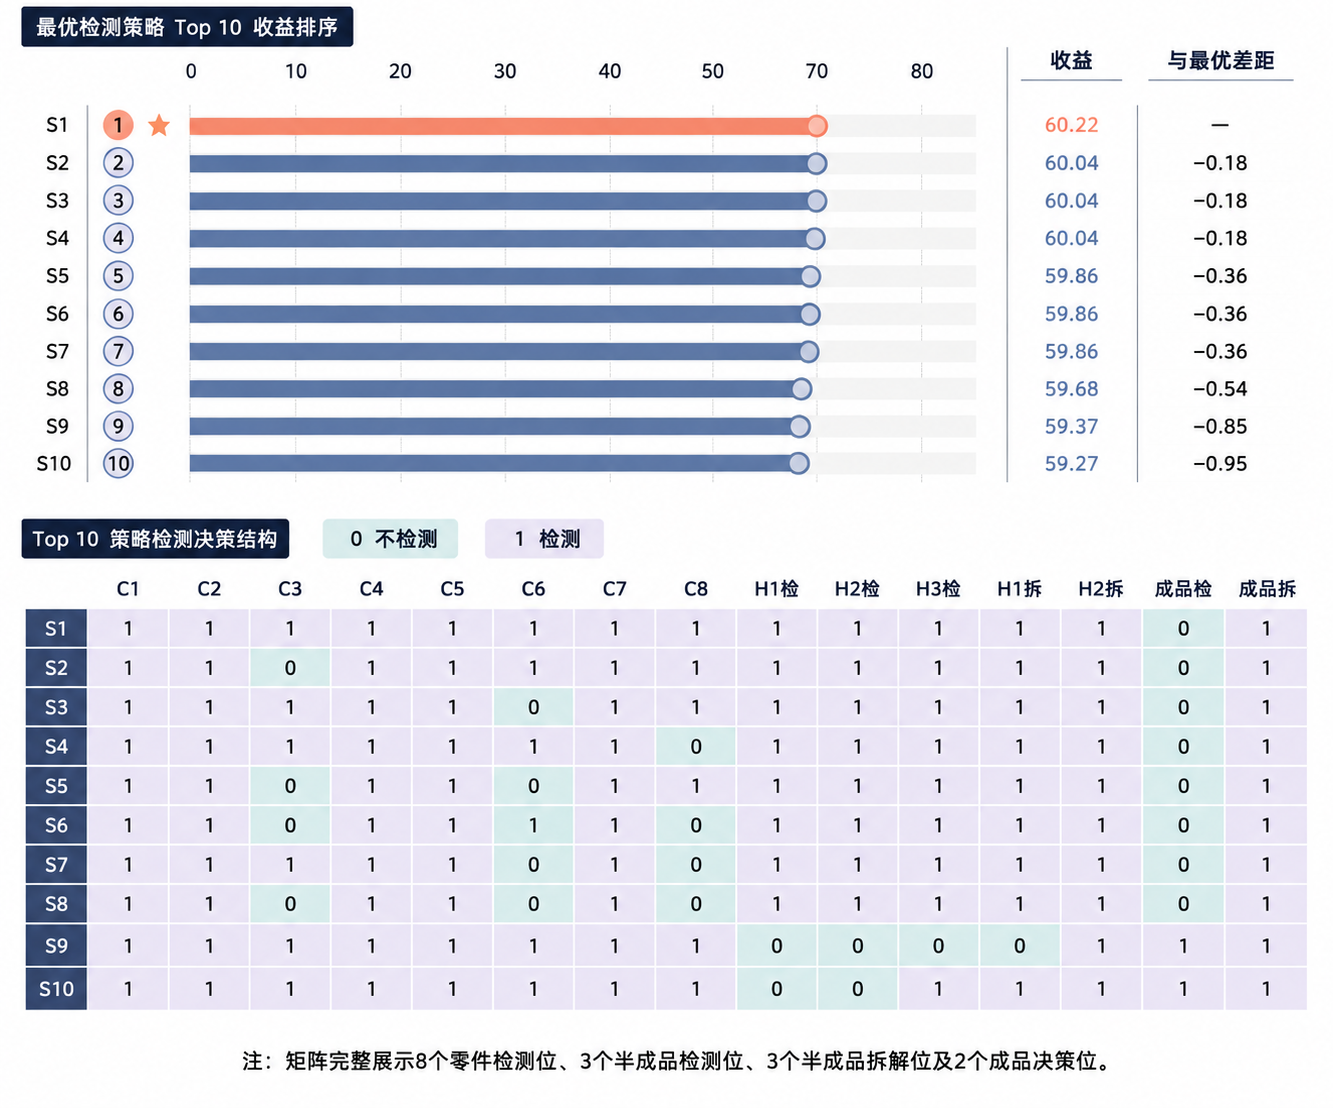
\includegraphics[width=0.85\textwidth]{figures/q3_fig4_top10.png}
    \caption{最优检测策略 Top 10 排序及决策结构}
    \label{fig:q3-top10}
\end{figure}
最优策略利润为 60.22 元，次优策略利润为 60.04 元，与最优解仅相差 0.18 元；排名第二至第四的策略主要是在 $C_3$、$C_6$ 或 $C_8$ 中取消一次零配件检测，而其余关键决策基本保持不变。收益条形排序与下方二元决策矩阵共同揭示：一方面，最优解附近存在若干收益十分接近的可替代方案，说明部分零配件检测决策处于成本—风险平衡的临界区域；另一方面，半成品检测与拆解、返件拆解等决策在高收益策略中高度一致，构成策略的稳定骨架。实际实施时可优先锁定这些稳定决策，再根据检测能力与产线负荷在 $C_3$、$C_6$、$C_8$ 的检测安排上小范围调整。



\textbf{（2）解析闭式与树形DP交叉验证}

将 BOM 分层递推的闭式解析结果与精确标量求解、树形 DP 三种独立实现分别比对：手算闭式与精确求解的利润差为 $0$，树形 DP 与扁平全枚举得到的最优策略完全一致（均为 \texttt{1111111111111101}），利润差亦为 $0$，成本分解之和与标量总成本的偏差约为 $2.8\times10^{-14}$。三种独立实现得到相同结果，说明状态压缩递推模型在数学上自洽、实现正确。

\textbf{（2）Monte Carlo 独立仿真验证}

对最优策略分别以 20 万笔向量化模拟与 1 万笔逐事件模拟估计单位期望利润。向量化模拟的均值误差为 60.18 元，$95\%$ 置信区间为 $[60.07,\ 60.29]$；逐事件模拟均值误差为 60.12 元，$95\%$ 置信区间为 $[59.62,\ 60.62]$。两种模拟下的理论期望利润 60.22 元均落入 $95\%$ 置信区间，且模拟得到的采购、半成品装配、成品装配、调换与拆解等事件次数与理论期望的绝对误差均小于 $0.01$。这表明仿真与解析模型不仅在总利润数值上一致，在内部流程层面亦吻合。收敛过程如图~\ref{fig:q3-mc}所示，随样本量增加，样本平均利润逐步贴近理论基准 60.22 元，置信区间同步收窄，说明偏差主要来自有限样本波动而非模型实现错误。

\begin{figure}[H]
    \centering
    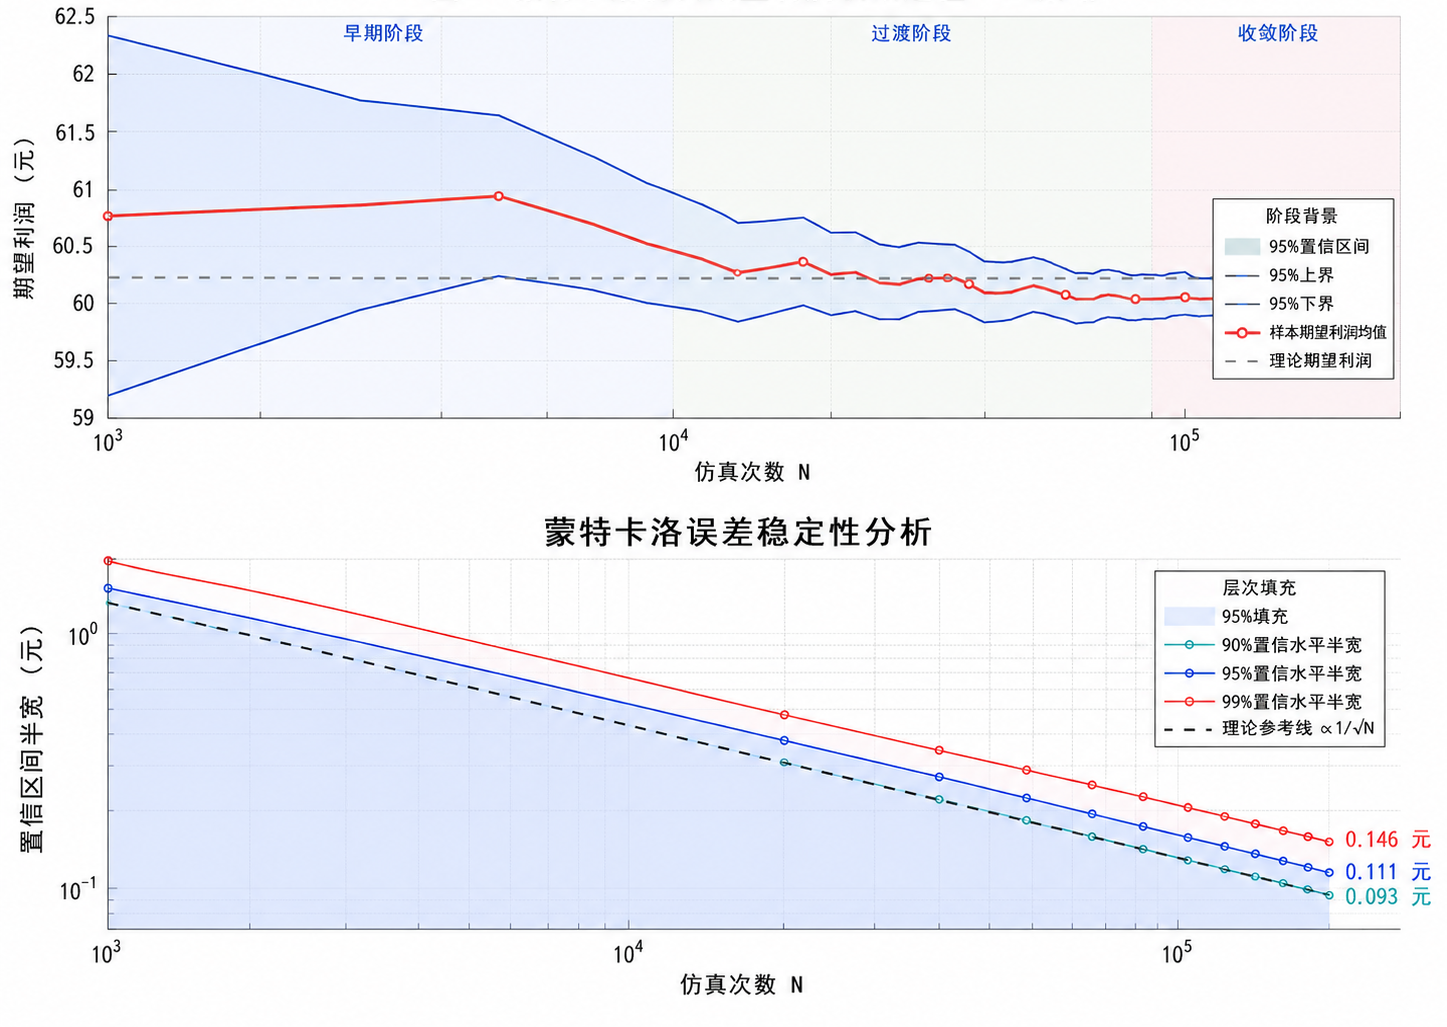
\includegraphics[width=0.85\textwidth]{figures/q3_fig7_mc.png}
    \caption{Monte Carlo 仿真期望利润收敛过程}
    \label{fig:q3-mc}
\end{figure}

\textbf{（4）极端情形检验}

构造四类极端参数场景验证模型行为是否符合经济学直觉：当所有次品率均为 $0$ 时，最优策略退化为全不检测、全不拆解（\texttt{0000000000000000}）；当调换损失极大时，最优策略开启成品检测（$y_F=1$）；当拆解成本极大时，最优策略关闭全部拆解动作（$z=0$）；当零配件检测成本极大时，最优策略关闭全部零件检测（$x_{Ci}=0$）。四种场景下模型的策略选择均与理论预期一致，验证了模型逻辑的正确性。

\textbf{（5）灵敏度分析}

对关键参数进行临界值扫描，得到最优策略的切换阈值。在零配件层面，各零配件检测成本 $b_{Ci}$（1~2 元）均低于其局部检测阈值 2.22 元，故检测各零件合理；半成品检测成本 $b_{Hj}=4$ 元低于阈值 7.16 元，故检测各半成品合理。在成品层面，调换损失 $L=40$ 元低于阈值 60 元、成品工序次品率 $p_F=0.1$ 低于阈值 0.15，故成品不检测合理；当 $L$ 超过 60 元或 $p_F$ 超过 0.15 时，最优策略将切换为对成品开展出厂检测。在拆解层面，半成品拆解成本 $d_{Hj}=6$ 元与成品拆解成本 $d_F=10$ 元均远低于其对应阈值（28.9 元、25.6 元与 125.3 元），故各拆解动作稳健。上述灵敏度结论与最优策略完全一致，再次验证了解的正确性与稳健性。

为更直观地刻画决策边界与参数影响，分别绘制参数相图与关键参数影响气泡图。图~\ref{fig:q3-phase}以关键参数的联合变化为坐标，用利润差刻画决策边界，可识别两个因素同时变化时的交互作用。全局重新优化得到的主要结构切换点为：调换损失约 47.68 元、成品不合格率约 0.1248、半成品检测成本约 5.30 元，均早于仅比较当前策略局部收益所得的理论阈值（调换损失 60 元、成品不合格率 0.15），原因是全局搜索允许多个决策同时变化，其他策略可能在局部决策尚未达到单点盈亏平衡前就率先超过基准策略。

\begin{figure}[H]
    \centering
    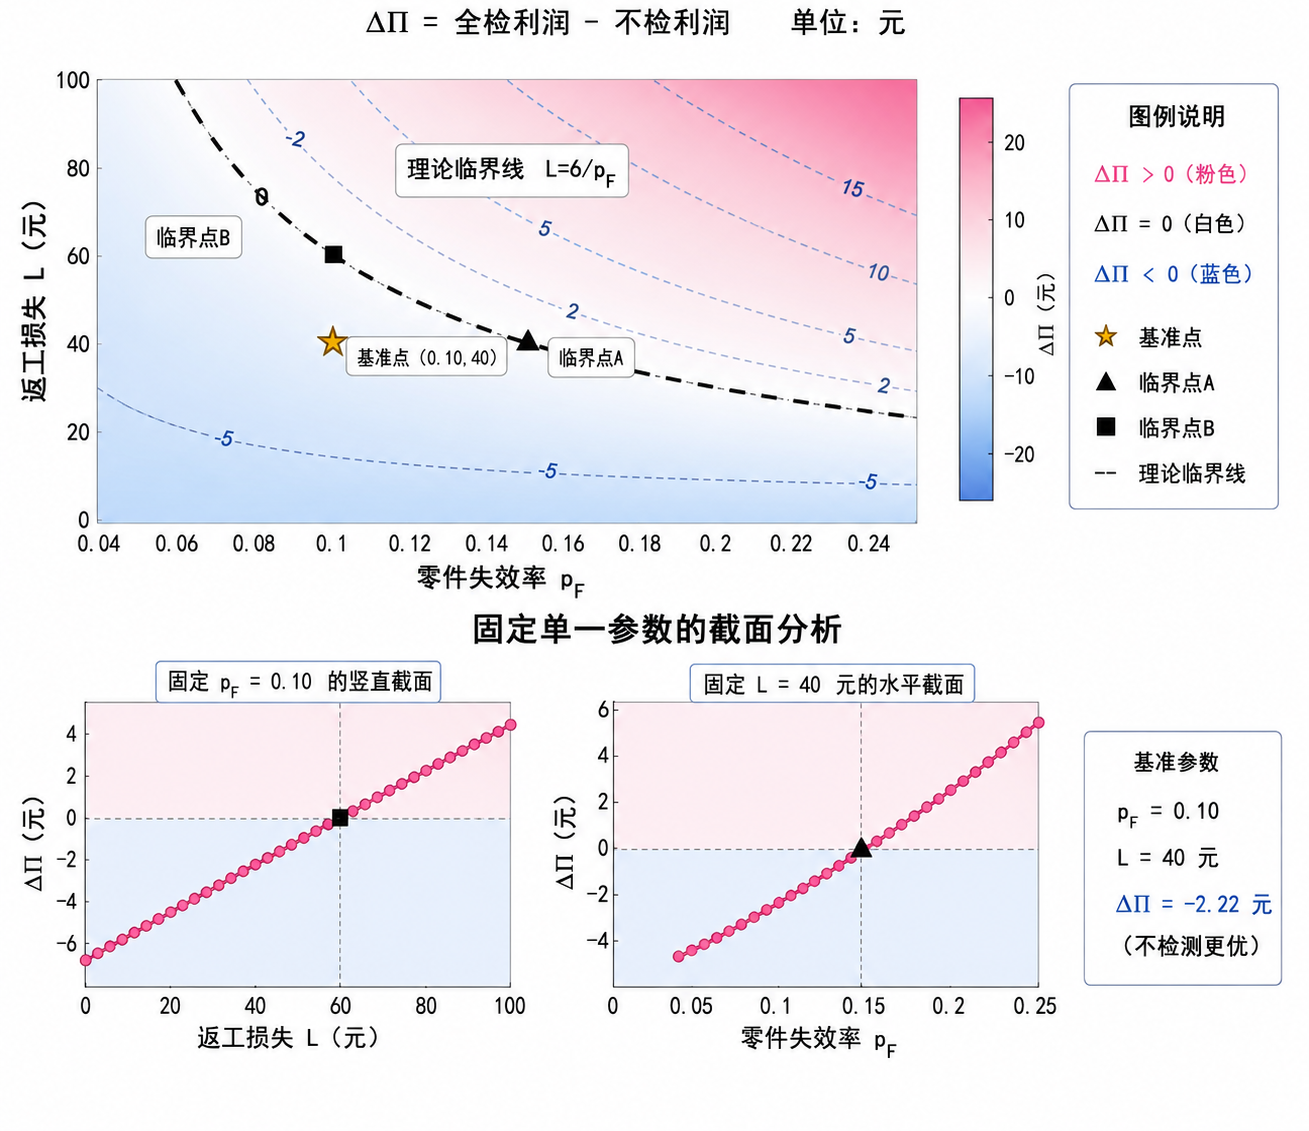
\includegraphics[width=0.85\textwidth]{figures/q3_fig5_phase.png}
    \caption{检测策略利润差参数相图}
    \label{fig:q3-phase}
\end{figure}

图~\ref{fig:q3-sens}以气泡图比较各关键参数的影响方向与幅度：横轴为参数相对基准值的变化范围，纵轴为不同参数，气泡颜色区分成本增加与降低，面积反映最优期望利润变化的绝对幅度。结果表明，直接改变投入或失效传播概率的参数（如材料单价、良品率、返工率）对利润影响更显著，检测时间、能耗等参数影响较弱；$C_3$、$C_6$、$C_8$ 当前检测费 2 元已接近约 2.22 元的局部阈值，与 Top 10 策略仅相差 0.18 元的现象相互印证。企业应优先监控高敏感参数，并对接近切换阈值的检测环节保留动态调整能力。

\begin{figure}[H]
    \centering
    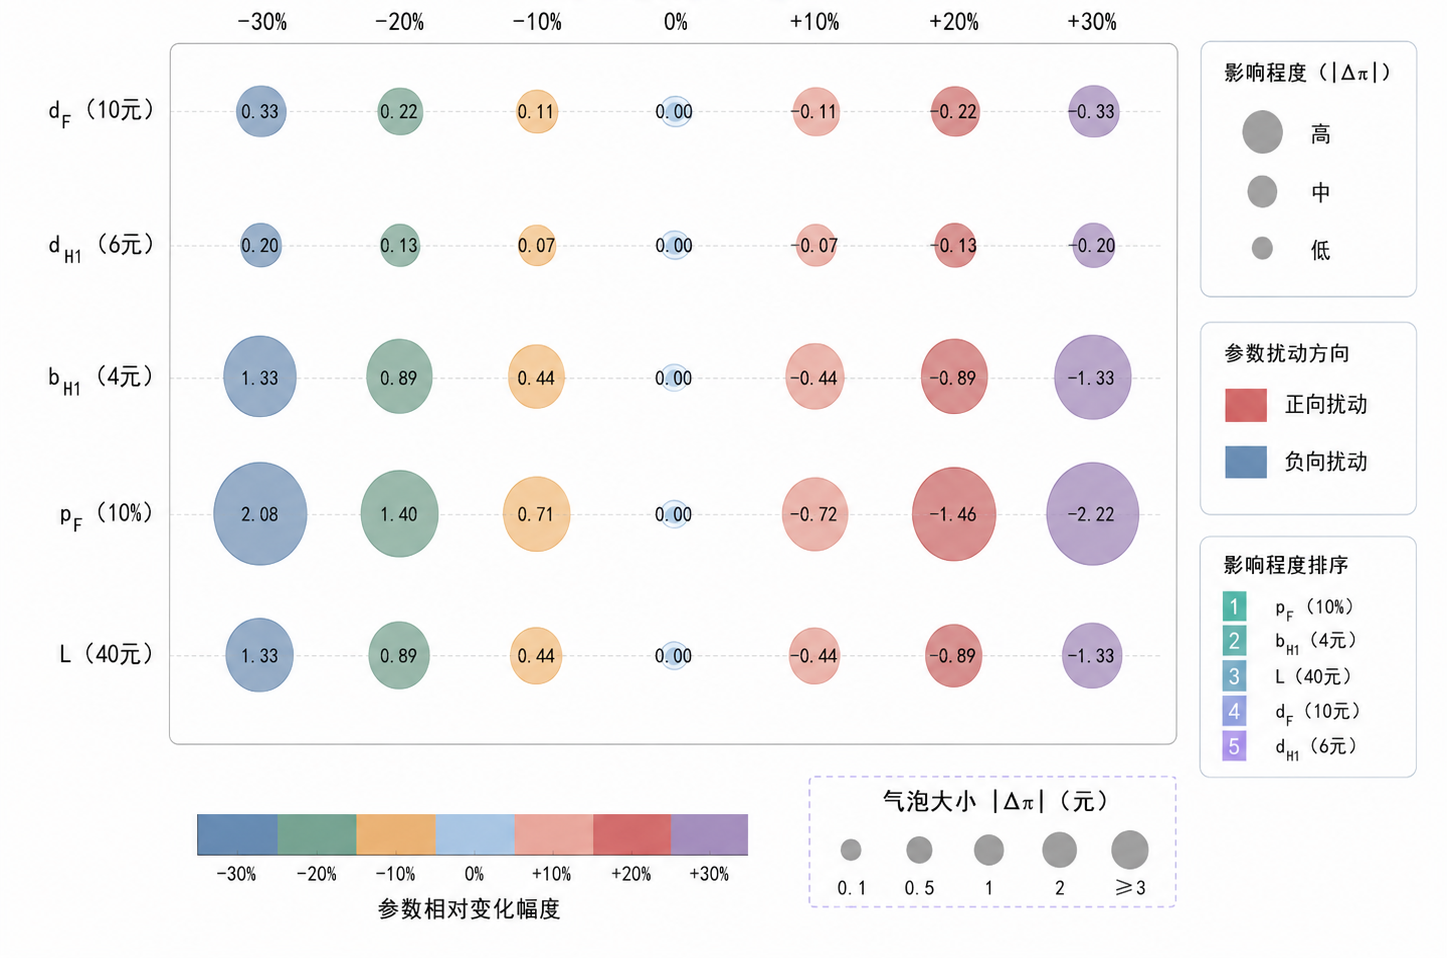
\includegraphics[width=0.85\textwidth]{figures/q3_fig6_sens.png}
    \caption{关键参数对最优期望利润的影响}
    \label{fig:q3-sens}
\end{figure}
\subsubsection{问题三的结论}

（1）问题三的最优生产方案为：八种零配件与三个半成品均检测、各半成品次品均拆解、成品不检测、用户退回次品拆解，对应期望成本\textbf{139.78 元}、期望利润\textbf{60.22 元}。此方案下，前端全面检测及早阻断质量风险，末端因三个半成品均已合格故不设检测反而更经济，各次品一律选择拆解以回收合格部件。

（2） 该模型结果经解析闭式、蒙特卡洛模拟、极端情形与灵敏度检验均一致，求解可靠，可为同类多工序、多零部件装配系统提供量化决策依据。
\subsection{问题四的模型建立与求解}












\subsubsection{问题四的模型建立}

问题四在前两问的基础上，将次品率由已知改为未知。因此需要在生产决策模型中引入统计不确定性。

\begin{enumerate}[itemindent=2em]
\item \textbf{次品率抽样推断模型} 

\hspace{2em}对每个质量参数，记真实次品率为 $p_j$，独立抽样 $n_j$ 件，检测结果 $X_{jt} \stackrel{\text{i.i.d.}}{\sim} B(p_j)$，累计次品数 $K_j = \sum_{t=1}^{n_j} X_{jt}$。则：
\begin{equation}
K_j \sim B(n_j, p_j), \quad \hat{p}_j = \frac{k_j}{n_j}.
\end{equation}
其中 $\hat{p}_j$ 为次品率的点估计值，可作为基准参数代入生产决策。但抽样估计存在不确定性，为控制决策风险，本文在风险水平 $\gamma$ 下计算置信上界 $U_j(\gamma)$。
\item \textbf{次品率置信上界模型}

\hspace{2em}沿用问题一的 e-process 序贯检验框架。由于每个质量参数均在证据充足即停止的规则下得到，其样本量 $n_j$ 本身即为随机停止时间，故对每个参数沿用问题一的单侧混合似然比证据 $E_{j,t}^-(p_0)$，将候选参数 $p_0$ 逐一作为原假设边界进行反演，得到对应的置信上界：
\begin{equation}
U_j^{\text{s}}(\gamma) = \inf\{ p_0 \in (0,1] : E_{j,t}^-(p_0) \ge\frac{1}{1-\gamma}  \}.
\end{equation}


\item \textbf{多次品率同时置信包络模型}

\hspace{2em}问题二每种情形含 $d=3$ 个不确定参数，问题三实例含 $d=12$ 个。为保证整个生产系统的所有质量参数同时落在上界内，采用 Bonferroni将总体风险 $\alpha = 1-\gamma$ 分配到各参数，令 $\alpha_j = \alpha/d$，构造系统级同时置信集合：
\begin{equation}
U_\gamma = \{ p : 0 \le p_j \le U_j^{\text{s}}(\gamma),\; j=1,\dots,d \}, \quad U_j^{\text{s}}(\gamma) = U_j(1-\alpha/d).
\end{equation}

该集合保证所有参数同时落在界内的概率不低于 $\gamma$，且不要求各参数独立。


\item \textbf{最坏次品率下的生产决策重优化模型}

\hspace{2em}将置信上界向量作为质量风险包络，代入前两问的精确评价器，在置信集合 $U_\gamma$ 上对所有候选策略重新优化。

\hspace{2em}沿用问题二、问题三的决策变量与精确评价器。在给定质量参数向量 $p$ 下，问题二解 Bellman 线性方程得到长期期望成本 $V_\pi(p)$，问题三由 BOM 分层递推得到根节点期望成本 $V_F(\pi; p)$。利润均记为：
\begin{equation}
\Pi_q(\pi; p) = S - V_q(\pi; p), \quad q = 2, 3.
\end{equation}

\hspace{2em}第四问在置信水平 $\gamma$ 下的核心目标函数为：
\begin{equation}
\pi_q^*(\gamma) = \arg\max_{\pi \in \Pi_q} \min_{p \in U_\gamma} \bigl[ S - V_q(\pi; p) \bigr], \quad q = 2, 3.
\end{equation}
约束条件为：
\begin{equation}
\text{s.t.}\quad
\begin{cases}
\pi \in \{0,1\}^d, \\
z=0 \Rightarrow r_1=r_2=0, \\
p \in U_\gamma, \\
\sup_{p \in U_\gamma} \rho\bigl(Q_\pi(p)\bigr) < 1.
\end{cases}
\end{equation}


\hspace{2em}目标函数中的内层取最小值，即在最坏质量参数下评估每个策略，是出于稳健性考虑：真实次品率未知，而生产决策一旦确定便难以中途调整，若仅以点估计优化，一旦真实质量恶化，原策略的利润将大幅下滑。因此在置信集合上考察每个策略的最坏表现，可保证所选策略无论真实次品率落在 $U_\gamma$ 内何处，利润都不低于该最坏值。

\hspace{2em}在本题生产结构下，任一质量参数 $p_j$ 增大只会使不合格品增多，从而抬升期望成本、压缩期望利润，而不会产生额外收益。因此固定策略的期望利润 $\Pi_q(\pi; p)$ 关于各缺陷概率具有单调非增性，即对 $p \preceq p'$ 有 $\Pi_q(\pi; p) \ge \Pi_q(\pi; p')$。由此置信集合 $U_\gamma$ 上的最坏点必落在各参数同时取上界处，可将最坏情形搜索简化为单点代入：
\begin{equation}
\min_{p \in U_\gamma} \Pi_q(\pi; p) = \Pi_q(\pi; U_\gamma^{\text{u}}).
\end{equation}

\item \textbf{ 稳健决策检验模型}

\hspace{2em}对于最优策略，还需判断当前样本信息是否足以支撑稳定决策。

\hspace{2em}一方面计算最优—次优利润间隔。设最优、次优策略分别为 $\pi_{(1)}$、$\pi_{(2)}$：
\begin{equation}
\Delta = \Pi(\pi_{(1)}) - \Pi(\pi_{(2)}), \quad \Delta_r = \frac{\Delta}{|\Pi(\pi_{(1)})|}.
\end{equation}

\hspace{2em}
若 $\Delta$ 很小，即使最优策略数学上唯一，实际采样稍有变化也可能更换策略。

\hspace{2em}另一方面采用与原抽样设计一致的  bootstrap 方法，固定样本按 $K^* \sim \text{Binomial}(n_j, \hat{p}_j)$ 重新抽样，序贯样本必须逐件生成 Bernoulli 流并复现问题一的停止规则。第 $b$ 次重抽样与重优化得到 $\pi_b^*$，则策略稳定率为：
\begin{equation}
R_\pi = \frac{1}{B} \sum_{b=1}^B I(\pi_b^* = \pi), \quad \text{SE}(R_\pi) = \sqrt{\frac{R_\pi(1 - R_\pi)}{B}}.
\end{equation}

\hspace{2em}当 $R_\pi$ 较高且 $\Delta$ 较大时，策略兼具经济优势与统计稳定性，可作为可靠决策采用；当 $R_\pi$ 较低或多个策略频率接近时，表明当前样本信息尚不足以固定单一最优策略，应以继续抽样缩小不确定性为管理建议。

\hspace{2em}此外，为分离质量参数恶化造成的损失与采用稳健策略付出的额外成本，引入四个交叉评价量。记 $\pi_N$ 为名义最优策略、$\pi_R$ 为稳健最优策略，$\hat{p}$ 为点估计向量，$U$ 为同时上界向量：
\begin{equation}
P_a = \Pi(\pi_N; \hat{p}), \quad P_b = \Pi(\pi_R; \hat{p}), \quad P_c = \Pi(\pi_N; U), \quad P_d = \Pi(\pi_R; U),
\end{equation}
\begin{equation}
P_e = P_a - P_b, \quad P_f = P_d - P_c, \quad P_g = P_a - P_c, \quad P_h = P_d.
\end{equation}
其中 $P_e$ 衡量名义状态下采用稳健策略少赚的利润，$P_f$ 衡量不利情形下稳健策略相对名义策略多保护的利润，$P_g$ 反映参数恶化本身造成的损失，$P_h$ 给出当前不确定集合下的最坏利润保证。该分解只用于解释既有最优策略，不改变目标函数。

\end{enumerate}















\subsubsection{问题四的求解结果}













\subsubsection{问题四的模型检验与结果分析}









%%%%%%%%%%%%%%%%%%%%%%%%%%%%%%%%%%%%%%%%%%%%%%%%%%%%%%%%%%%%%
\section{模型的评价、改进与推广}

\subsection{模型的优点}
\begin{itemize}[itemindent=2em]
\item 优点1
\item 优点2
\item 优点3
\end{itemize}

\subsection{模型的缺点}
\begin{itemize}[itemindent=2em]
\item 缺点1
\item 缺点2
\end{itemize}




\subsection{模型的改进}






\subsection{模型的推广}










\section{AI工具使用声明}

本参赛队在竞赛过程中使用了AI工具，主要用于语言润色、代码调试，详细使用情况见支撑材料。













\begin{thebibliography}{99}

   
    \bibitem{lidaqian2014}
    李大潜.
    从数学建模到问题驱动的应用数学[J].
    \textit{数学建模及其应用}, 2014, 3(1).


\end{thebibliography}


























\newpage
%% 附录
\begin{appendices}
	
	
	
	
\section{文件列表}
\begin{table}[H]
\centering
\begin{tabularx}{\textwidth}{LL}
\toprule
文件名   & 功能描述 \\
\midrule
%%%%%%%%%%%%%%%%%%%%%%%%%%%%%%%%%%%%%%%%%%%%%%%%%%%%%%%%%%%%%
数据预处理.py & 预处理程序代码 \\
q2.py & 问题二程序代码 \\
q3.c & 问题三程序代码 \\
q4.cpp & 问题四程序代码 \\
%%%%%%%%%%%%%%%%%%%%%%%%%%%%%%%%%%%%%%%%%%%%%%%%%%%%%%%%%%%%%
\bottomrule
\end{tabularx}
\label{tab:文件列表}
\end{table}






\newpage

%\section{代码}
%\noindent 
%%%%%%%%%%%%%%%%%%%%%%%%%%%%%%%%%%%%%%%%%%%%
%数据预处理.py
%\lstinputlisting[language=python]{code/1.数据预处理.py}
%%%%%%%%%%%%%%%%%%%%%%%%%%%%%%%%%%%%%%%%%%%%%
%
%%%%%%%%%%%%%%%%%%%%%%%%%%%%%%%%%%%%%%%%%%%%
%q2.py
%\lstinputlisting[language=python]{code/q2.py}
%%%%%%%%%%%%%%%%%%%%%%%%%%%%%%%%%%%%%%%%%%%%
%
%
%q3.c
%\lstinputlisting[language=c]{code/q3.c}
%
%
%q4.cpp
%\lstinputlisting[language=c++]{code/q4.cpp}

\end{appendices}
\end{document}
